%%UTF-8
\documentclass[twoside,UTF8]{nputhesis}
%\documentclass[oneside]{nputhesis}
\usepackage{mathptmx}
\usepackage{amsmath}
\usepackage{amsfonts}
\usepackage{booktabs}
\usepackage{multirow}

\usepackage{subfigure}
\usepackage{bm}
\usepackage{lipsum}
\usepackage{enumerate}
\usepackage{ listings} 
\usepackage{amsthm}

\usepackage{graphicx}
\usepackage{epstopdf}

\usepackage{longtable}
\newcommand{\upcite}[1]{\textsuperscript{\textsuperscript{\cite{#1}}}}
\usepackage[linesnumbered,boxed,ruled,commentsnumbered]{algorithm2e}
\usepackage{algorithm, algorithmic}
\usepackage{cite}

\usepackage{titlesec}



%%算法包,注意设置所需可选项






%标题和chapte


\schoolno{10699}
\classno{O242}
%\secretlevel{}
\title[Numerical Simulation for the Fractional Monodomain Model of Cardiac Potential]{  心脏电势分数阶单域模型数值模拟}
\author[Zhaoru Zhang]{张昭儒}
\authorno{2017202152}


\major[Computational Mathematics]{计算数学}
\supervisor[Cai Li]{蔡力}
\applydate[March 2020]{2020~年~3~月}
%\support{本文研究得到xxxxxx项目资助。}

\begin{document} 


\makecover  % 中英文封面
\frontmatter
 \captionsetup{font={small}}
% 中文摘要
\begin{abstract}
心脏疾病是目前危及人类生命健康安全的最危险的疾病之一,其发病率及致死率呈逐年上升的趋势。通过数值模拟心脏电生理过程已成为研究心脏生理过程及病理特征的重要手段。考虑到分数阶导数的非局部特性及在反常扩散领域中的广泛应用,分数阶FHN模型能更加合理地刻画心脏介质上的跨膜电势传播过程。在粒子反常扩散扩散过程中,受到扩散区域的限制或者细胞本身生命周期的限制,有向服从标准扩散统计规律转变的趋势,而回火分数阶导数可以灵活地刻画这一过程。本文建立了回火分数阶FHN模型用于描述心肌细胞跨膜电势传播过程,并建立了无条件稳定的有限差分格式计算模型。

首先,本文结合回火分数阶微积分基本理论,应用有限差分方法建立了对回火Riesz分数阶导数算子的数值逼近格式,进而建立le针对回火分数阶FHN模型的有限差分格式进行计算。

其次,由于实际问题中计算区域一般比较复杂并且分数阶导数具有非局部特性,导致系数矩阵的阶数非常大,并且通常为稠密矩阵。应用传统计算方法计算这种大规模稠密矩阵方程组需要消耗巨大的计算成本。本文应用R. Chan循环预处理算法及预处理共轭梯度法(PCG),大幅度提高了计算效率。同时,本文对于有限差分格式进行修改,使其能够在不规则区域上进行计算。

最后,通过数值算例验证了有限差分方法的数值误差及空间收敛阶。在不同区域、回火指数、分数阶阶数及扩散系数条件下计算二维回火FHN模型,成功模拟了跨膜电势在不同条件下的传播规律。
\noindent
\begin{keywords}
  回火分数阶FHN模型,有限差分法,预处理共轭梯度法
\end{keywords}
\end{abstract}

% 英文摘要
\begin{Abstract}
	
Heart disease is one of the most dangerous diseases that endanger human health and safety, and its morbidity and mortality are increasing year by year. Numerical simulation of the cardiac electrophysiological model has become an important method for studying the physiological processes and pathological characteristics of the heart. Considering the non-local characteristics of fractional derivative and its extensive application in the field of anomalous diffusion, the fractional FHN model can more reasonably simulate the transmembrane potential propagation process on cardiac media. Due to the restriction of diffusion region and cell life cycle, the anomalous diffusion eventually relaxes into a traditional diffusion profile at last time, this tendency is also called transient anomalous diffusion. The tempered fractional derivative can flexibly describe this process. In this paper, a tempered fractional FHN model is established to describe the transmembrane potential transmission process of cardiomyocytes, and an unconditionally stable finite difference scheme calculation model is established.

Firstly, application the basic theory of tempered fractional calculus, this paper uses the finite difference method to establish a numerical discrete scheme for tempered Riesz fractional derivative operators and then constructs an finite difference scheme for tempered fractional FHN models. 

Secondly, because the fractional derivatives have non-local characteristics and the computational domain is generally complicated in practical problems, the order of the coefficient matrix is ​​very large, and it is usually a dense matrix. Applying traditional calculation methods to calculate such large-scale dense matrix equations requires huge calculation costs. In this paper, the R. Chan loop preprocessing algorithm and preprocessing conjugate gradient method are used to greatly improve the calculation efficiency. At the same time, this paper modified the finite difference scheme to enable it to perform calculations on irregular regions.

Finally, numerical examples are used to verify the numerical error and spatial convergence order of the finite difference method. Considering the factors such as changing the calculation area, tempering index, fractional-order and diffusion coefficient, the tempered fractional FHN model was calculated under different conditions to successfully simulate the propagation law of transmembrane potential under different conditions.

    \begin{Keywords}
      Tempered fractional FHN model,Finite difference method,Pretreatment conjugate gradient 
    \end{Keywords}
\end{Abstract}

% 目录
\tableofcontents 

\mainmatter  

\chapter{绪论}
\section{研究背景与意义}
心脏通过维持血液流遍全身,运送营养物质及氧气到各个细胞之中并携带代谢废物离开,以维持人类正常的生理活动与代谢运转。心脏性疾病致死人数约占总死亡人数的30\%,取代冠状动脉疾病及中风成为人类最常见的致死性疾病之一。由于心脏疾病通常情况下没有明显的病症表现,对于心脏病的诊断需要有经验的医师结合病史,应用超声波设备、心电图及听诊器等手段进行经验性的判断。这种方式误诊率高,容易延误病患的治疗时机。心脏数值模拟技术做为心脏疾病临床诊治的重要手段,受到研究者们的广泛关注。

对于心脏生理及病理的传统研究方法都是基于心肌细胞、载体蛋白及基因等微观层面进行研究分析,只能反映单细胞及分子水平微观特性,无法深入解释心脏疾病的发病过程及生理变化情况。目前针对心脏疾病的诊治更多的依赖于医师经验性的判断,误诊率较高。心脏数值模拟作为连接心肌细胞微观电生理变化与心脏宏观病症表现的桥梁,有效地提高了心脏疾病的诊断与医治效率\upcite{fenton2005modeling,mcculloch1992large,lesh1989cellular}。心脏数值模拟是一项结合生物化学、解剖学、流体力学、计算机科学及数学等学科的复杂的综合系统工程,通过应用计算机科学技术与数学相关算法,数值仿真心脏相关生理活动及病理变化,为心脏疾病的临床诊治提供了重要途径\upcite{shuaiby2013finite,groenendaal2015cell,bernus2002computationally,ten2006comparison,nickerson2010cardiac}。

心脏数值模拟主要可以分为电生理模拟与非电生理模拟两个方向。本文主要研究心脏电生理模拟过程。心脏电势传播过程的数值模拟是心脏数值模拟中重要的组成部分\upcite{Fitzhugh1961Impulses},其通过电势分布情况判断电流是否通过心脏,是否有效地控制心脏收缩与舒张,并判断特殊药物对于心脏的影响。通过这一过程可以对心率失常发病过程进行有效地判断。心肌细胞的的电兴奋传导主要依赖于细胞膜的离子通道对于特殊离子的选择通透性。数值模拟心肌细胞受到外界刺激产生电势传播规律对于特殊心脏疾病的诊治及心脏疾病治疗药物的研究等方面都有重要的意义。

\subsection{心肌细胞的跨膜电势}
心肌组织是由心肌细胞与细胞间隙构成,心脏电生理过程依赖跨膜电势的产生与传播。心肌细胞跨膜电势的产生本质上是细胞膜对于特殊离子的选择通透性导致离子分布短时间发生改变造成的。细胞膜是由磷脂双分子层与蛋白质构成,由磷脂双分子层组成的薄膜阻碍离子顺浓度梯度进行扩散运动,而细胞膜上镶嵌的载体蛋白起到了离子通道的作用,载体蛋白允许特殊离子顺浓度梯度进行跨膜运动,离子通道的开启与关闭会在细胞膜内外造成短暂的电位变化。由于细胞膜内钾($\mathrm{K}^{+}$)离子浓度高于细胞膜外,钾离子外流导致静息状态下细胞膜两侧的电位分布内负外正。当细胞膜受到电刺激,钠($\mathrm{Na}^{+}$)离子载体蛋白通道打开,钠离子内流导致膜两侧的电位分布出现短暂的内正外负,此过程称为去极化过程。此后,钾离子持续外流使电位差迅速恢复到零,随之钙离子通道打开,钙离子内流,部分抵消了钾离子外流的效果,使得电位差缓慢下降至-90mv左右,完成复极化过程。细胞复极化过程完成后,细胞膜两侧离子浓度趋于稳定,恢复至静息状态。                                                                                                                                                                           

\subsection{FHN单域模型}

对于心肌细胞跨膜电势的数值模拟需要考虑离子通道的开闭过程。传统模型仅能实现对离子通道关于时间及电刺激强度依赖性的模拟,无法解释可兴奋性、刺激阈值及不应期这些电势传播过程中特殊的现象及概念。1928年,van der Pol与van der Mark\upcite{van1928lxxii}两人使用类似于振荡器的电路模型模拟心肌细胞的电生理过程,并考虑了离子通道受到的刺激阈值。但由于模型过于简单,未受到研究者们广泛地关注与重视。随后,Hodgkin与Huxley两人通过对于枪乌贼巨神经轴突上的膜离子电流与电导进行研究,于1963年连续发表文章阐述各类组织中兴奋扩散与组织细胞间相互作用的关系,并将细胞及其膜上的各类离子通道简化为电阻电路模型,模拟膜电位随时间变化的情况,这便是著名的Hodgkin-Huxley(HH)模型\upcite{hodgkin1952quantitative}。HH模型的提出对后续细胞电生理研究带来深远的影响,现有的大多数心肌细胞电生理模型都是基于Hodgkin与Huxley两人的研究工作而来的\upcite{fitzhugh1961impulses,van1980computer}。随后,Noble使用非线性电阻替代线性电阻模拟钾离子通道,实现电导内向整流及外向整流\upcite{noble1962modification,noble1998improved}。HH模型是由四个主要变量组成的非线性微分方程组,模型计算困难,对计算结果分析复杂。20世纪中期,Fitzhugh依据实践经验发现,与钠离子相比,钾离子离子通道激活概率与抑制概率的变化率较小,因此钠离子的激活概率可以使用平衡状态的值替代,而钾离子的激活概率与抑制概率的和维持在0.8左右。其依据这一事实,对于HH模型进行合理简化\upcite{Fitzhugh1961Impulses}。Nagumo在模拟电路中添加二极管模拟放电行为\upcite{nagumo1962active}。经过Fitzhugh与Nagumo对于HH模型的不断简化与改进,最终建立著名心脏单域电生理模型—FitzHugh-Nagumo(FHN)模型\upcite{fitzhugh1955mathematical}。该模型由一个空间带有拉普拉斯算子的扩散方程与常微分方程耦合而成,模拟了神经细胞受到电刺激时产生的电兴奋传播过程。作为HH模型的简化模型,FHN模型被广泛地应用于神经元放电行为的模拟研究中。

\subsection{分数阶FHN单域模型及回火分数阶导数} 

目前针对心肌组织电兴奋传播规律已经建立了广泛的理论研究基础,其中应用最为普遍的是单域(Monodomain)模型与双域(Bidomain)模型。双域模型最早是由Schmitt提出的\upcite{schmitt1969biological}。随后,Tung\upcite{tung1978bi}应用扩散方程模拟电兴奋扩散规律,并给出了双域模型的数学定义。其核心思想是将心肌组织划分成心肌细胞内区域与细胞外区域两个独立的部分,在不同部分施加独立的电刺激,使用反应扩散方程模型分别模拟细胞内外在受到电刺激条件下电兴奋传播规律。由于双域模型的计算涉及对大规模矩阵的求逆运算,为了节省计算开销,研究者们假设细胞膜内外具有相同的各向异性,并将细胞膜内外当成一个整体进行计算,由此构造出单域模型。研究表明,单域模型与双域模型关于模拟电兴奋传导的计算结果差异不大\upcite{potse2006comparison}。常见的单域及双域模型都是假设心肌组织是由纤维组织集合而成的片状结构,细胞间隙与细胞质之间具有较强的一致性。但是普遍认为心脏是一个不连续的非均匀多孔介质,细胞质的扩散尺度存在较大的差异,细胞间隙与细胞质之间具有较强的抵抗性。而细胞质的不连续性是造成心肌组织之间非均匀性的根本原因。心脏动作电位是由离子在心肌细胞中跨膜运动而产生的,受到组织空间中非均匀异质性结构的限制,粒子传播不在服从标准扩散规律\upcite{bueno2014fourier}。因此,传统单双域模型不再适用于模拟心脏电兴奋传播规律\upcite{ying2005multilevel, bueno2014fractional},为此引入并构造了带有分数阶导数的单域模型。分数阶导数因非局部特性及在模拟反常扩散现象中的卓越表现,受到研究者们广泛地关注与重视。分数阶导数广泛应用于物理\upcite{rudolf2000applications,magdziarz2007fractional,mainardi2010fractional,
	metzler2000random,metzler2004restaurant,piryatinska2005models,
	tarasov2008fractional}、经济\upcite{gorenflo2001fractional,jurlewicz2009coupled,
mainardi2000fractional,meerschaert2006coupled,scalas2000fractional,
scalas2006five}、生物\upcite{baeumer2007fractional,barkai2012single,fedotov2007migration,
jeon2012anomalous}及水文地理学\upcite{baeumer2001subordinated,benson2000application,benson2001fractional,
cushman2000fractional,deng2006parameter,schumer2001eulerian}等问题的研究中。
Ying等人\upcite{ying2005multilevel}构造空间分数阶微分算子模拟离子在非均匀介质条件下的传播过程。Ochaoa-Tapia等人\upcite{valdes2006effective}提出了分数阶Darcy定律,并将其用于模拟非均匀介质中的剪应力现象。Cushman等人\upcite{cushman1994nonequilibrium}提出了分数阶Fick定律模拟高度各向异性多孔介质扩散现象。随后,其结合分数阶Fick定律,构造出分数阶FHN模型模拟心肌细胞跨膜电势中传播规律\upcite{liu2013numerical,liu2013numerical1}。目前已有多种关于分数阶FHN模型的数值计算方法提出。Zeng等人\upcite{zeng2014crank}通过使用谱方法进行计算。Bu等人\upcite{bu2014galerkin,bu2015finite}结合隐式Garlerkin有限元方法及Crank-Nicolson(CN)方法计算分数阶FHN模型。Cai等人\upcite{Guo2018Nonstandard}结合多重网格法与非标准有限差分法对分数阶FHN模型进行高效数值计算。Liu等人\upcite{liu2002unstructured,liu2003two,LiuA}在非结构化网格上应用有限体积法计算齐次Neumann条件下二维分数阶反应扩散方程。针对分数阶FHN模型中引入的Riesz分数阶导数,Liu等人\upcite{liu2013numerical}构造出了一阶精度的有限差分格式。随后,Liu\upcite{liu2015semi}对其进行修改,应用有限差分方法在不规则区域上计算分数阶FHN模型。Wang\upcite{wang2019simulation}构造虚拟结构体,可在不规则区域上计算心脏单域模型。

反常扩散现象是指自由系统中的粒子不再服从Fick扩散规律的扩散行为。研究者们定义跳跃步长与等待时间两种指标刻画粒子反常扩散行为。结合分数阶微积分相关理论,Sokolov等人\upcite{klafter2005anomalous}构造出了分数阶反常扩散模型:$\partial _{t}^{\beta }p(x,t)=\partial _{x}^{\alpha }p(x,t)$ ,其中空间分数阶导数$\alpha<2$称为扩散指数,用于描述自由粒子的跳跃步长服从的重尾幂率关系$P[J>x]\approx {{x}^{-\alpha }}$,时间分数阶导数$\beta <1$对应描述自由粒子的等待时间,其服从的重尾幂率关系$P[W>t]\approx {{t}^{-\beta }}$。一般通过时间分数阶导数刻画亚扩散现象(Sub-diffusion),空间分数阶导数描述超扩散现象(Super-diffusion)\upcite{sabzikar2015tempered}。在自由粒子反常扩散过程中,受到扩散区域及粒子生命周期的限制,粒子扩散规律有向服从标准扩散统计规律转化的趋势,这一过程称为“暂态反常扩散”过程(Transient anomalous diffusion)\upcite{bronstein2009transient}。通过在控制反常扩散行为的幂律关系中添加指数因子,可以推导一种新的分数阶导数定义形式——回火(Tempered)分数阶导数\upcite{baeumer2010tempered}。应用回火分数阶导数构造的扩散方程可以用于模拟“暂态反常扩散”过程。空间回火分数阶导数对粒子空间跳跃步长幂律分布关系加以控制,使其概率密度函数呈现半重尾分布特征。同理,通过调控等待时间幂律分布关系可以推导出时间回火分数阶导数。粒子跳跃步长幂律分布呈重尾分布的随机游走现象称为Lévy飞行\upcite{mandelbrot1983fractal, metzler2004restaurant, meerschaert2008tempered},为了模拟半重尾分布Lévy飞行,Koponen等人\upcite{koponen1995analytic}使用指数因子对幂率分布关系加以截断。为保证截断效果光滑性,Rheinwald等人\upcite{rheinwald1973transmissible}应用回火分数阶扩散方程模拟Lévy飞行模型。Mantegna与Stanley\upcite{mantegna1994stochastic}发现回火随机游走模型的跳跃步长幂律分布关系最终会收敛到回火稳定状态,而这种回火稳定状态趋近于服从标准扩散统计规律\upcite{barndorff1997processes}。Mantegna与Stanley发现证明了反常扩散最终有向正常扩散转化的趋势,应用回火分数阶导数能够有效地模拟这种趋势。目前针对回火分数阶扩散方程高精度数值计算方法的研究工作方兴未艾\upcite{li2016high}。Deng及其团队\upcite{li2016high, yu2017third, dehghan2017fourth}针对空间带有回火分数阶导数的扩散方程提出过多种高精度数值计算方法。


\subsection{分数阶微分方程快速计算与Toeplitz系统预处理方法}

分数阶反应扩散方程是模拟粒子反常扩散的有力工具,但实际问题中计算区域一般比较复杂并且分数阶导数具有非局部特性,导致系数矩阵的阶数非常大,并且通常为稠密矩阵。应用传统计算方法计算这种大规模稠密矩阵方程组需要消耗巨大的计算成本。例如在计算过程中使用共轭梯度法等数值方法产生的计算量为$O({{n}^{3}})$\upcite{golub1996cf},由于该算法计算量主要来源矩阵向量乘,对矩阵合理优化可以大幅度提高计算效率。目前已有多种针对分数阶扩散方程的高效数值算法出现。例如针对分数阶扩散方程数值计算方法导出的特殊Toeplitz线性系统,Wang等人\upcite{wang2010direct}提出快速算子分裂方法,将计算量降至$O(n{{\log }^{2}}(n))$。Wang\upcite{wang2011fast}结合Douglas与Russel的研究成果\upcite{douglas1982numerical}提出了快速特征有限差分法,将计算量进一步降至$O(n\log (n))$。另一方面,基于Toeplitz线性系统矩阵预处理方法的研究工作在过去20年得到了飞速地发展\upcite{chan2007introduction, jin2003developments, ng2004iterative}。Strang\upcite{strang1986proposal}提出的循环预处理矩阵可以大幅度缩减求解一些良态Hermite-Toeplitz线性系统的计算量。T.Chan\upcite{chan1988optimal}提出的最优循环预处理矩阵不仅针对Toeplitz线性系统,对于一般良性的矩阵系统也可以提升计算效率。而对于病态Toeplitz系统,R.Chan等人\upcite{chan1995best}提出了一种针对性循环预处理方案。


\section{本文的研究内容}
本文主要研究心脏电生理过程的数值仿真,受到心脏非均匀介质的影响,电势传播规律不再服从标准扩散统计规律,故建立了回火分数阶FHN模型更加合理地刻画心脏介质上的跨膜电势传播过程。本文主要针对回火分数阶FHN模型的高效数值模拟方法的构建进行研究。

本文章节简介如下:

第一章为绪论部分,简要介绍了数值模拟心肌细电生理过程研究背景及研究意义,着重介绍了分数阶FHN模型的定义形式及回火分数阶导数的研究现状,并总结了本文的主要研究内容。

第二章为回火分数阶FHN模型,首先介绍了几种回火分数阶导数的定义,并从随后从心肌细胞反应扩散模型出发,依次介绍了整数阶FHN模型及分数阶FHN模型的定义形式及特点,最终结合回火分数阶为基本基本理论建立了回火分数阶FHN模型及相应的初边值条件。

第三章为回火分数阶FHN模型的数值模拟,首先应用有限差分法构建模型的的离散格式,并对有限差分格式进行修改,使其能够在不规则区域上进行计算。最后,本章应用预处理共轭梯度法计算离散格式转化的矩阵方程,大幅度提高了计算效率。

第四章为数值实验,通过数值算例验证了有限差分方法的数值误差及空间收敛阶。在不同区域、回火指数、分数阶阶数及扩散系数条件下计算二维回火FHN模型,成功模拟了跨膜电势在不同条件下的传播规律。

第五章为总结与展望部分,主要对于本文的研究内容进行简要概括,对于未来的研究方向及内容作出展望。                            







\chapter{回火分数阶FHN单域模型}
本章主要介绍心肌细胞的跨膜电势传播模型。首先介绍了整数阶FHN模型的构造形式及其物理意义。由于心脏的非均匀多孔介质结构从根本上改变了自由粒子扩散所服从的标准扩散规律,呈现出不规则扩散规律。考虑到分数阶导数的非局部特性及在模拟反常扩散问题上卓越表现,应用分数阶FHN模型可以更加真实的刻画心脏介质上电势传播规律。在自由粒子反常扩散的过程中,受到扩散区域及粒子细胞生命周期的限制,粒子扩散规律有向服从标准扩散规律转化的趋势,本文应用带有回火分数阶导数的扩散方程模拟这一过程。回火分数阶导数通过添加回火指数控制回火程度。本文将标准分数阶FHN模型中的Riesz分数阶导数替换为回火Riesz分数阶导数,推导出二维回火分数阶FHN模型,并列出了模型的初边值条件及相应的生理学意义。

\section{回火分数阶导数的基本理论}

分数阶微积分理论作为数学的一个重要分支,得到相关学者们的广泛关注与研究。针对不同的应用场景,先后建立了如Riemann-Liouville(R-L)分数阶导数、Grünwald–Letnikov(G-L)分数阶导数及Caputo等一系列完备的分数阶导数定义形式。回火分数阶导数是在原有分数阶导数定义上延拓出的新的分数阶导数定义,其在特殊条件下可以退化为相应的分数阶导数定义。本节主要介绍几种常见的回火分数阶导数定义。

Gamma函数$\Gamma(z)$是分数阶计算的基本函数。Gamma函数是对于阶乘函数$n!$的推广,允许$n$的取值为整数、非整数及复数。\\
\noindent   %当行不缩进
\textbf{定义2.1}
第二类Euler积分\upcite{Temme1997Special}:
\begin{equation}
\Gamma(z)=\int_{0}^{+\infty} x^{z-1} e^{-x} d x, \quad \operatorname{Re}(z)>0
\end{equation}
称为Gamma函数。这里$z$为一个复数,$Re(z)$为复数$z$实部的取值。
利用分部积分公式,Gamma函数存在以下递推关系:
\begin{equation}
\Gamma(z+1)=z \Gamma(z), \quad \operatorname{Re}(z)>0
\end{equation}
如果$-n<\operatorname{Re}(z) \leq-n+1$(这里$n$为一个正整数),那么:
\begin{equation}
\Gamma(z)=\frac{\Gamma(z+n)}{z(n)}=\frac{\Gamma(z+n)}{z(z+1) \cdots(z+n-1)}
\end{equation}
Gamma函数存在以下性质:\\
(1) $\Gamma(0)=1$,且对于任意正整数$n$,有$\Gamma(n)=(n-1)!$\\
(2) 对于任意正整数$n$,有
\begin{equation}
\begin{array}{l}{\Gamma(z+n)=(z)_{n} \Gamma(z)} \\ {\Gamma(z-n)=\frac{\Gamma(z)}{(z-n)_{n}}=\frac{(-1)^{n}}{(1-z)_{n}} \Gamma(z)\quad (z \neq 1,2,3, \cdots)}\end{array}
\end{equation}
(3) $\Gamma(1 / 2)=\sqrt{\pi}$

\noindent   %当行不缩进
\textbf{定义2.2}(回火R-L分数阶导数)\upcite{sabzikar2015tempered,于妍妍2016(回火的)分数阶扩散方程的差分数值算法}:
\\
假设$u(x)\in C[a,b]$且有足够的正则性,那么对于任意$\lambda \ge 0$,$m-1<\alpha <m\quad(m\ge 1,m \in \mathbb{N}^{+})$,则$\alpha $阶左、右回火R-L分数阶导数定义为
\begin{equation}
\begin{split}
&{}_{a}D_{x}^{(\alpha ,\lambda )}u(x)={{e}^{-\lambda x}}{}_{a}D_{x}^{\alpha }({{e}^{\lambda x}}u(x))=\frac{{{e}^{-\lambda x}}}{\Gamma (m-\alpha )}\frac{{{d}^{m}}}{d{{x}^{m}}}\int_{a}^{x}{{{(x-s)}^{m-\alpha -1}}{{e}^{\lambda s}}u(s)ds}
\end{split}
\end{equation}
%
\begin{equation}
\begin{split}
&{}_{x}D_{b}^{(\alpha ,\lambda )}u(x)={{e}^{\lambda x}}{}_{x}D_{b}^{\alpha }({{e}^{-\lambda x}}u(x))=\frac{{{(-1)}^{m}}{{e}^{\lambda x}}}{\Gamma (m-\alpha )}\frac{{{d}^{m}}}{d{{x}^{m}}}\int_{x}^{b}{{{(s-x)}^{m-\alpha -1}}{{e}^{-\lambda s}}u(s)ds}
\end{split}
\end{equation}

从上式可以看出,首个等式关系表示回火R-L分数阶导数与标准R-L分数阶导数存在联系。回火导数添加带有变量$\lambda$的指数函数调控回火程度,称$\lambda$为回火指数,当$\lambda =0$时回火R-L分数阶导数退化为标准R-L分数阶导数。而第二个等式关系表示与标准R-L分数阶导数的定义形式类似,回火R-L分数阶导数使用积分形式定义,设计数值计算方法存在困难,为此引入回火G-L分数阶导数的概念。

如上定义所示,回火R-L分数阶导数使用积分形式定义,为了方便构造数值离散格式,引入级数形式定义的G-L分数阶导数进行数值逼近\upcite{li2016high,meerschaert2004finite}。Meerschaert指出\upcite{meerschaert2004finite},应用标准G-L分数阶导数构造计算空间分数阶微分方程的数值格式是无条件不稳定的,故此引入移位G-L分数阶导数的概念。由于回火G-L分数阶导数可以被认为是标准G-L分数阶导数在定义形式上的延拓,为了保持构造离散格式的一致性,数值计算方法沿用回火移位G-L分数阶导数\upcite{tadjeran2007second}进行计算。\\
\noindent   %当行不缩进
\textbf{定义2.3}(回火移位G-L分数阶导数)\upcite{li2016high,meerschaert2004finite}:
\\
假设$1<\alpha <2$,$u(x)\in {{C}^{n+3}}[a,b]$且对于$u(x)$的各阶导数有$\frac{d^k{u(x)}}{dx^k}\in {{L}^{1}}[a,b](k=0,1,\cdots ,n+3)$。对于任意整数$p$和$\lambda \ge 0$,$\alpha$阶左回火移位G-L分数阶导数定义如下:
\begin{equation}
_{a}\emph{\textbf{D}}_{x,p}^{(\alpha ,\lambda )}u(x)=\lim _{h \rightarrow 0} \frac{1}{h_{x}^{\alpha}} \sum_{k=0}^{\left\lceil(x-a) / h_{x}+p\right\rceil} g_{k}^{(\alpha)} e^{-(k-p) \lambda h_{x}} u\left(x-(k-p) h_{x}\right)
\end{equation}
其与左回火R-L分数阶导数存在如下联系:
\begin{equation}
\begin{split}
&_{a}\emph{\textbf{D}}_{x,p}^{(\alpha ,\lambda )}u(x) ={}_{a}D_{x}^{(\alpha ,\lambda )}u(x)+
\sum\limits_{l=1}^{n-1}{\left( c_{p,l}^{(\alpha)}{}_{a}D_{x}^{(\alpha +l,\lambda )}u(x){h_{x}^{l}} \right)}+O({h_{x}^{n}})
\end{split}
\end{equation}

上面回火分数阶导数的定义对于任意$x\in[a,b]$一致成立。权重系数$g_{k}^{(\alpha )}=\Gamma (k-\alpha )/\left( \Gamma (-\alpha )\Gamma (k+1) \right)$为函数${{(1-z)}^{\alpha }}$级数展开的系数,而$c_{p,l}^{(\alpha) }$为函数${{\left( (1-{{e}^{z}})/z \right)}^{\alpha }}{{e}^{pz}}$的级数展开的系数,$h_{x}$为空间步长。从等式(2-7)可以看出,当$\lambda =0$时回火移位G-L导数退化为移位G-L分数阶导数,当位移量$p=0$时,移位G-L分数阶导数完全退化为标准G-L分数阶导数。从定义形式可以看出,左回火移位G-L分数阶导数是将左标准回火G-L导数的计算单元整体向右移动整数$p$步得到的。等式(2-8)则说明回火移位G-L分数阶导数可以写成关于不同分数阶阶数的回火R-L分数阶导数之和的形式。                              当$n=1$时,利用回火G-L分数阶导数建立对于回火R-L分数阶导数一阶数值逼近。右回火移位G-L分数阶导数定义形式如下:
\begin{equation}
_{x}\emph{\textbf{D}}_{b,p}^{(\alpha ,\lambda )}u(x)=\lim _{h_{x}\rightarrow 0} \frac{1}{h_{x}^{\alpha}} \sum_{k=0}^{\left\lceil(b-x) / h_{x}+p\right\rceil} g_{k}^{(\alpha)} e^{-(k-p) \lambda h_{x}} u\left(x+(k-p) h_{x}\right)
\end{equation}
\noindent
\textbf{性质2.1}:权重系数$\text{ }\!\!\{\!\!\text{ }g_{k}^{(\alpha )}\text{ }\!\!\}\!\!\text{ }$存在递推关系\upcite{刘发旺2015分数阶偏微分方程数值方法及其应用}:
\begin{equation}
g_{0}^{(\alpha)}=1,\quad g_{k}^{(\alpha)}=\left(1-\frac{\alpha+1}{k}\right) g_{k-1}^{(\alpha)}\quad (k=1,2, \cdots)
\end{equation}
服从如下性质:\\
当$1<\alpha <2$时,
\begin{equation}
\begin{split}
& g_{0}^{(\alpha )}=1,\quad g_{1}^{(\alpha )}=-\alpha,\quad g_{2}^{(\alpha )}>g_{3}^{(\alpha )}>\cdots >0, \\
& \sum\limits_{k=0}^{\infty }{g_{k}^{(\alpha )}}=0,\quad \sum\limits_{k=0}^{m}{g_{k}^{(\alpha )}}<0\quad (m\ge 1)
\end{split}
\end{equation}
当$\alpha =2$时,
\begin{equation}
\begin{split}
g_{0}^{(\alpha )}=1,\quad g_{1}^{(\alpha )}=-2,\quad g_{2}^{(\alpha )}=1,\quad g_{3}^{(\alpha )}=g_{4}^{(\alpha )}=\cdots =0
\end{split}
\end{equation}

根据本文需要,引入回火Riesz分数阶导数定义形式。\\
\textbf{定义2.4}
(回火Riesz分数阶导数)\upcite{邬小超2016回火反常运动粒子轨迹泛函分布的建模,ervin2006variational,roop2004variational,cartea2007fluid}:\\
假设函数$u(x)\in {{L}^{1}}[a,b]$,那么对于任意$\lambda \ge 0$,$m-1<\alpha <m \quad(m\ge 1,m\text{为正整数})$,定义回火Riesz分数阶导数:
\begin{equation}
\begin{split}
\frac{{{\partial }^{(\alpha ,\lambda )}}}{\partial {{\left| x \right|}^{(\alpha ,\lambda )}}}u(x)=-\frac{1}{2\cos (\alpha \pi /2)}({}_{a}D_{x}^{(\alpha ,\lambda )}u(x)+{}_{x}D_{b}^{(\alpha ,\lambda )}u(x))
\end{split}
\end{equation}
当$\lambda =0$时回火Riesz分数阶退化为标准Riesz分数阶导数。其中${}_{a}D_{x}^{(\alpha ,\lambda )}u(x)$、${}_{x}D_{b}^{(\alpha ,\lambda )}u(x)$为左、右回火R-L分数阶导数。

\section{心肌细胞的反应扩散模型}
生物电生理过程中,将心肌细胞及大脑皮层细胞这类受到电刺激能够产生明显反应的细胞称为可兴奋细胞。可兴奋细胞能够定时生成和传播电兴奋信号,调节组织器官的生理过程。当可兴奋细胞接受电刺激产生兴奋时,细胞膜内外的电解质分布会因为细胞膜的通透性变化而改变。细胞接受电刺激而在受刺激处细胞膜两侧产生一次快速而可逆的电位变化称为动作电位。在生物学中,通常使用反应扩散方程模拟离子跨膜运动。
反应扩散方程又称为激励传播动力学模型,是由一系列非线性微分方程耦合而成,能够有效的模拟受刺激组织细胞的电兴奋传播过程。反应扩散方程的一般形式如下:
\begin{equation}
\frac{\partial u_{i}}{\partial t}=\nabla \cdot\left(D_{i} \nabla u_{i}\right)+f_{i}\left(u_{1}, \cdots, u_{n}\right) \quad i=1,2, \cdots n
\end{equation}
其中$u_{i}$为状态变量,$f_{i}$与$D_{i}$分别为源项函数与扩散系数。在心肌细胞电势传播模型中,状态变量$u_{i}$表示跨膜电势的状态变化。在电兴奋传播模拟过程中,细胞状态的变化由源项函数$f_{i}$及扩散项$\nabla \cdot\left(D_{i} \nabla u_{i}\right)$共同决定。

心肌细胞组织由心肌细胞与细胞间隙组成,扩散系数建立了二者之间的联系。如果假设心脏组织细胞内外为均匀统一的介质,通过电流传播模型计算细胞内部电流源密度$f_{i}$并根据电流源密度$f_{i}$更新细胞的电生理状态来模拟心脏电生理传播过程。假设定源项函数表示通过细胞膜内外离子通道的总电流$I_{ion}$,则可定义整数阶FHN单域模型。作为模拟心肌细胞电兴奋传播模拟的简化模型,二维无量纲整数阶FHN单域模型构造如下:
\begin{equation}
\frac{\partial u}{\partial t}=\nabla \cdot(K \nabla u)+I_{i o n}(u, v)
\end{equation}
\begin{equation}
\frac{\partial v}{\partial t}=a u-b v+c
\end{equation}
\begin{equation}
I_{i o n}=\frac{C_{2}}{u_{a n p}}\left(u-u_{r e s t}\right) v+\frac{C_{1}}{u_{a m p}^{2}}\left(u-u_{r e s t}\right)\left(u-u_{t h}\right)\left(u-u_{p e a k}\right)
\end{equation}
其中$u$表示标准跨膜电势,$v$表示与时间相关的无量纲恢复变量,$K$表示以张量形式表示的扩散系数,而非负参数$a$、$b$、$c$、$C_{1}$与$C_{2}$设置为标准化取值0.13、0.013、1、0.26与0.1。
尽管整数阶FHN单域模型在模拟电生理过程的研究中已取得了不少成果,但传统建模方法普遍假设空间传播介质为连续均匀的介质,复合组织结构对于空间的电兴奋传导的影响可以忽略不计,在模拟复杂组织结构上电势传播问题上存在较大的局限性。首先,心脏肌细胞形成的集合细纤维排列呈现片状结构。针对这一特点,可以假设细胞质与细胞间隙具有连续性,在广泛的空间尺度上可以假设组织结构为均匀的介质区域。但据已有的研究结果表明,哺乳动物的组织细胞中细胞质的局部空间尺度的不连续性是造成心肌细胞非均匀的根源。此外, 细胞的连接方式对于电兴奋传导传播形式存在影响。因此,整数阶单域模型在模拟心肌细胞电生理过程存在局限。

在这样研究背景下,整数阶反应扩散模型不在适用于模拟心脏组织的电兴奋传导机制。由于分数阶导数非局部特性及遗传效应,分数阶反应扩散方程在模拟反常扩散问题上的卓越表现,使用分数阶反应扩散方程模拟不均匀介质下的合并多尺度效应的传送过程成为一个合适的选择。为了模拟具有高度各向异性的多孔介质结构上的电势传播过程,在整数阶FHN模型中添加Riesz分数阶算子,可以获得二维分数阶FHN模型:
\begin{equation}
\frac{\partial u}{\partial t}=K R^{\alpha} u+I_{ion}(u, v)
\end{equation}
其中$R^{\alpha}=\left(R_{x}^{\alpha}, R_{y}^{\alpha}\right)=\left(\partial^{\alpha} / \partial|x|^{\alpha}, \partial^{\alpha} / \partial|y|^{\alpha}\right)$为Riesz分数阶算子,Riesz分数阶导数是分数阶Laplace算子一种特殊的表达形式\upcite{zhang2018riesz}。扩散方程右端源项函数$I_{ion}$与关于变量$v$的常微分方程定义形式与整数阶FHN模型保持一致。与整数阶FHN模型相比,分数阶FHN模型能够捕捉在具有高度各向异性的多孔介质条件下的空间组织间转送的信息,适用于模拟心肌组织的电势传播规律。

心脏区域电势传播是特殊离子反常扩散作用的结果,考虑到分数阶反应扩散方程在模拟反常扩散问题上的卓越表现,故构造分数阶FHN模型进行数值模拟。另一方面,在粒子反常扩散过程中,受到扩散空间或者细胞生命周期的限制,离子扩散规律有向服从标准扩散规律转化的趋势,即自由粒子的随机运动符合Gauss统计规律,这一转化的过程称为"暂态反常扩散"。在原有控制分数阶扩散方程的幂律关系上添加指数函数,可以推导出一种新的分数阶导数定义形式——回火分数阶导数。回火分数阶扩散方程可以用于模拟这一过程。空间回火分数阶导数对粒子空间跳跃步长幂律分布关系加以控制,使其概率密度函数呈现半重尾分布特性。为了真实模拟心脏介质上因区域局限与异质性引起的介于正常扩散与反常扩散之间特殊的电势传播规律,本文将分数阶FHN模型中Riesz分数阶导数替换为回火Riesz分数阶导数,建立回火分数阶FHN模型:
\begin{equation}
\frac{\partial u}{\partial t}={{K}_{x}}\frac{{{\partial }^{({{\alpha }_{1}},{{\lambda }_{1}})}}u}{\partial {{\left| x \right|}^{({{\alpha }_{1}},{{\lambda }_{1}})}}}+{{K}_{y}}\frac{{{\partial }^{({{\alpha }_{2}},{{\lambda }_{2}})}}u}{\partial {{\left| y \right|}^{({{\alpha }_{2}},{{\lambda }_{2}})}}}+{{I}_{ion}}(u,v)
\end{equation}

其中$\frac{{{\partial }^{({{\alpha }_{i}},{{\lambda }_{i}})}}\bm{u}}{\partial {{\left| x \right|}^{({{\alpha }_{i}},{{\lambda }_{i}})}}}\quad(i=   1\text{、}2)$为回火Riesz分数阶导数,${{\lambda }_{1}}$、${{\lambda }_{2}}$分别为控制$x$及$y$方向上回火程度的回火指数,为了方便计算,本文设置$\lambda=\lambda_{1}=\lambda_{2}$,分数阶$1<{{\alpha }_{1}},{{\alpha }_{2}}\le 2$。整数阶常微分方程与右端源项函数的定义形式与式(2-16)-(2-17)相同。从上式可以看出,回火分数阶FHN模型由空间带有回火Riesz分数阶导数的扩散方程与整数阶常微分方程耦合而成,数值模拟回火Riesz分数阶导数成为计算模型的关键。

\section{回火Riesz分数阶耦合系统}
考虑到回火分数阶FHN系统是由扩散方程与整数阶常微分方程耦合而成,系统中计算方法的稳定性及收敛性受到各个方程数值解的共同影响,需要对其进行综合分析。为了进一步探究系统计算方法及算法的稳定性与收敛性,在有限区域$[0,D_{x}]\times[0,D_{y}]$上建立由回火Riesz分数阶偏微分方程与常微分方程耦合而成的系统模型如下:
\begin{equation}
\frac{\partial u}{\partial t}=K_{x} \frac{\partial^{\left(\alpha_{1} \lambda\right)} u}{\partial|x|^{\left(\alpha_{1}, \lambda\right)}}+K_{y} \frac{\partial^{\left(\alpha_{2}, \lambda\right)} u}{\partial|y|^{\left(\alpha_{2}, \lambda\right)}}+f(u, v,x,y,t)
\end{equation}
\begin{equation}
\frac{d v}{d t}=g(u,v,x,y,t)
\end{equation}
其中方程右端源项函数$f(u,v,x,y,t)$及$g(u,v,x,y,t)$关于$u$与$v$在有界区域$\Omega$连续。定义系统的初值条件如下:
\begin{equation}
\begin{aligned}
&u(x, y, 0)=\phi(x, y)\\
&v(x, y, 0)=\psi(x, y)\quad(x, y) \in \Omega
\end{aligned}
\end{equation}
边界条件置为零Dirichlet边界条件为:
\begin{equation}
\begin{aligned}
&u(0, y, t)=u\left(D_{x}, y, t\right)=u(x, 0, t)=u\left(x, D_{y}, t\right)=0\\
&v(0, y, t)=v\left(D_{x}, y, t\right)=v(x, 0, t)=v\left(x, D_{y}, t\right)=0\\
\end{aligned}
\end{equation}






\section{本章小结}
本文从心肌细胞反应扩散方程入手,首先介绍了在有限区域上的整数阶FHN单域模型的构造形式及生理学意义。在此基础上,从传播介质的特殊性出发阐述了传统模型在模拟非均匀多孔介质上的粒子扩散过程中的弊端。由于分数阶反应扩散方程在模拟反常扩散问题上的卓越表现,引入由空间带有Riesz分数阶算子的扩散方程构造的分数阶FHN模型模拟心脏区域上的电兴奋传播规律。考虑到扩散空间对于离子扩散行为的限制,本文将分数阶扩散方程中Riesz分数阶算子替换为回火Riesz分数阶算子,进而建立了回火分数阶FHN模型模拟跨膜电势在心肌细胞的传播规律。

\chapter{回火分数阶FHN模型的数值模拟}
本章主要研究回火分数阶FHN模型的数值计算方法的建立过程。本文应用有限差分方法对于耦合方程进行计算。此外,本章对于有限差分方法进行修改,使其能够在不规则区域上进行计算。最后,针对回火分数阶FHN模型有限差分格式所转化的矩阵方程$A\bm{x}=\bm{b}$进行计算。由于实际问题中计算区域一般比较复杂并且分数阶导数具有非局部特性,导致系数矩阵的阶数非常大,并且通常为稠密矩阵。应用传统计算方法计算这种大规模稠密矩阵方程组需要消耗巨大的计算成本,本章应用R.Chan所构造的预处理共轭梯度法进行计算,极大地提高了计算效率。

\section{回火Riesz分数阶耦合系统有限差分格式的构造}
本节主要研究回火分数阶FHN模型中回火扩散方程的有限差分格式的构造方法,通过对于方程中回火Riesz分数阶导数应用不同精度的数值逼近建立相应的有限差分格式,时间方向上应用向后Euler格式进行计算。

为了构造数值离散格式,定义空间区域$\Omega \text{= }\!\![\!\!\text{ 0,}{{\text{D}}_{x}}\text{ }\!\!]\!\!\text{ }\times \text{ }\!\![\!\!\text{ 0,}{{\text{D}}_{y}}\text{ }\!\!]\!\!\text{ }$及时间区域$[0,T]$并网格剖分,取空间步长及时间步长分别为${{h}_{x}}={{D}_{x}}/{{m}_{1}}$、${{h}_{y}}={{D}_{y}}/{{m}_{2}}$和$\tau =T/N$,相应的${{x}_{i}}=i{{h}_{x}}(i=0,1,\cdots ,{{m}_{1}})$、${{y}_{j}}=j{{h}_{y}}(j=0,1,\cdots ,{{m}_{2}})$、${{t}_{n}}=n\tau(n=0,1,\cdots ,N)$。定义$u_{i,j}^{n}$为$u({{x}_{i}},{{y}_{j}},{{t}_{n}})$的数值近似,初始条件为$u_{i,j}^{0}=\phi ({{x}_{i}},{{y}_{j}})$。

结合定义2.3,建立左(右)回火R-L分数阶导数的一阶数值逼近格式:
\begin{equation}
\begin{split}
&{}_{a}D_{x}^{(\alpha ,\lambda )}u({{x}_{i}},{{y}_{j}},{{t}_{n}})=\frac{1}{{{h}_{x}^{\alpha }}}\sum\limits_{l=0}^{i+1}{g_{l}^{(\alpha )}}{{e}^{-(l-1)\lambda {h}_{x}}}u({{x}_{i-l+1}},{{y}_{j}},{{t}_{n}})+O({h}_{x})
\end{split}
\end{equation}
\begin{equation}
\begin{split}
&{}_{x}D_{b}^{(\alpha ,\lambda )}u({{x}_{i}},{{y}_{j}},{{t}_{n}})=\frac{1}{{{h}_{x}^{\alpha }}}\sum\limits_{l=0}^{{{m}_{1}}-i+1}{g_{l}^{(\alpha )}}
{{e}^{-(l-1)\lambda {h}_{x}}}u({{x}_{i+l-1}},{{y}_{j}},{{t}_{n}})+O({h}_{x})
\end{split}
\end{equation}

结合定义2.4回火Riesz分数阶导数的定义,建立一阶数值离散格式:
\begin{equation}
\frac{\partial^{\alpha_{1}, \lambda}}{\partial|x|^{\alpha_{1}, \lambda}} u\left(x_{i}, y_{j}, t_{n}\right)=-r_{1}\left[\sum_{l=0}^{i+1} g_{l}^{(\alpha_{1})}{{e}^{-(l-1)\lambda {h}_{x}}} u\left(x_{i-l+1}, y_{j}, t_{n}\right)+\sum_{l=0}^{m_{1}-i+1} g_{l}^{(\alpha_{1})
}{{e}^{-(l-1)\lambda {h}_{x}}} u\left(x_{i+l-1}, y_{j}, t_{n}\right)\right]+O\left(h_{x}\right)
\end{equation}
其中${{r}_{1}}={{K}_{x}}{{c}_{{{\alpha }_{1}}}}/{{({{h}_{x}})}^{{{\alpha }_{1}}}}$,${{r}_{2}}={{K}_{y}}{{c}_{{{\alpha }_{2}}}}/{{({{h}_{y}})}^{{{\alpha }_{2}}}}$,${{c}_{\alpha }}=1/[2\cos (\pi \alpha /2)]<0$,$y$方向上的回火Riesz分数阶导数数值离散格式构造类似。

更进一步,为了建立回火R-L分数阶导数的二阶数值离散格式,引入以下命题:\\
\noindent
\textbf{命题3.1}:$u(x)\in {{C}^{5}}[a,b]$,且$u(x)$直到5阶导数属于${{L}_{1}}[a,b]$,对于任意$p\ne q$,左回火R-L导数存在2阶数值逼近:
\begin{equation}
\begin{split}
{{s}_{1}}_{a}\emph{\textbf{D}}_{x,p}^{(\alpha ,\lambda )}u(x)+{{s}_{2}}_{a}\emph{\textbf{D}}_{x,q}^{(\alpha ,\lambda )}u(x)u(x)={}_{a}D_{x}^{(\alpha ,\lambda )}u(x)+O({h_{x}^{2}})
\end{split}
\end{equation}
对于$\forall x\in[a,b]$一致成立,其中${{s}_{1}}=\frac{\alpha -2q}{2(p-q)}$,${{s}_{2}}=\frac{2p-\alpha }{2(p-q)}$。\\
证明:由式(2-8)可得
\[
\begin{split}
& {{s}_{1}}_{a}\emph{\textbf{D}}_{x,p}^{(\alpha ,\lambda )}u(x)+{{s}_{2}}_{a}\emph{\textbf{D}}_{x,q}^{(\alpha ,\lambda )}u(x)
=({{s}_{1}}+{{s}_{2}}){}_{a}D_{x}^{(\alpha ,\lambda )}u(x)+({{s}_{1}}c_{1}^{\alpha ,p}+{{s}_{2}}c_{1}^{\alpha ,q}){}_{a}D_{x}^{(\alpha +1,\lambda )}u(x)+O({h_{x}^{2}}) \\
\end{split}
\]
对于$\forall x\in[a,b]$一致成立,令:
\[\left\{ \begin{split}
& {{s}_{1}}+{{s}_{2}}=1 \\
& {{s}_{1}}c_{1}^{\alpha ,p}+{{s}_{2}}c_{1}^{\alpha ,q}=0 \\
\end{split} \right.\]
已知$c_{1}^{\alpha ,p}=p-\alpha /2$, $c_{1}^{\alpha ,q}=q-\alpha /2$,则可以解得:
\[{{s}_{1}}=\frac{\alpha -2q}{2(p-q)} \qquad  {{s}_{2}}=\frac{2p-\alpha }{2(p-q)}\]
右回火R-L分数阶导数的数值逼近关系同理可得。$\hfill\qedsymbol$\\     %添加方框,右对齐

上述命题表明,应用不同位移量的回火G-L分数阶导数进行加权组合可以构造回火R-L分数阶导数高阶数值逼近格式。本文在$\alpha \in (1,2)$条件下,取$(p,q)=(1,0)$,应用命题3.1得${{s}_{1}}=\frac{\alpha }{2}$,${{s}_{2}}=\frac{2-\alpha }{2}$并代入式(3-5),得到回火R-L分数阶导数的二阶数值逼近格式:
\begin{equation}
\begin{split}
&{{s}_{1}}_{a}\emph{\textbf{D}}_{x,p}^{(\alpha ,\lambda )}u(x)+{{s}_{2}}_{a}\emph{\textbf{D}}_{x,q}^{(\alpha ,\lambda )}u(x)
=\frac{\alpha }{2}{_{a}\emph{\textbf{D}}_{x,1}^{(\alpha ,\lambda )}u(x)}+(1-\frac{\alpha }{2}){_{a}\emph{\textbf{D}}_{x,0}^{(\alpha ,\lambda )}u(x)}  \\
&=\frac{\alpha }{2}{h_{x}^{-\alpha }}\sum\limits_{k=0}^{\infty }{g_{k}^{(\alpha )}}{{e}^{-(k-1)\lambda h_{x}}}u(x-(k-1)h_{x}  )
+(1-\frac{\alpha }{2}){h_{x}^{-\alpha }}\sum\limits_{k=0}^{\infty }{g_{k}^{(\alpha )}}{{e}^{-k\lambda h_{x}}}u(x-kh_{x}  )  \\
&={h_{x}^{-\alpha }}\sum\limits_{k=0}^{\infty }{w_{k}^{(\alpha )}}u(x-(k-1)h_{x}  )
={}_{a}D_{x}^{(\alpha ,\lambda )}u(x)+O({h_{x}^{2}})  \\
\end{split}
\end{equation}
其中权重系数$\{w_{k}^{(\alpha )}\}$满足递推关系:
\[w_{0}^{(\alpha )}=\frac{\alpha }{2}g_{0}^{(\alpha )}{{e}^{\lambda h_{x}}}\]
\[w_{k}^{(\alpha )}=\frac{\alpha }{2}g_{k}^{(\alpha )}{{e}^{-(k-1)\lambda h_{x}}}+(1-\frac{\alpha }{2})g_{k-1}^{(\alpha )}{{e}^{-(k-1)\lambda h_{x}}}\quad(k\ge 1)\]
结合定义2.4构造回火Riesz分数阶导数二阶数值离散格式:
\begin{equation}
\frac{\partial^{\alpha_{1}, \lambda}}{\partial|x|^{\alpha_{1}, \lambda}} u\left(x_{i}, y_{j}, t_{n}\right)=-r_{1}\left[\sum_{l=0}^{i+1} w_{l}^{(\alpha_{1})} u\left(x_{i-l+1}, y_{j}, t_{n}\right)+\sum_{l=0}^{m_{1}-i+1} w_{l}^{(\alpha_{1})
} u\left(x_{i+l-1}, y_{j}, t_{n}\right)\right]+O\left(h_{x}^{2}\right)
\end{equation}
其中$r_{\mathrm{l}}$、$r_{\mathrm{2}}$定义同上,对于y方向上的回火Riesz导数离散形式类似。












对于方程(2-20)右端非线性源项函数近似如下\upcite{liu2013numerical}:
\begin{equation}
\begin{split}
f(u({{x}_{i}},{{y}_{j}},{{t}_{n}}),v({{x}_{i}},{{y}_{j}},{{t}_{n}}),{{x}_{i}},{{y}_{j}},{{t}_{n}})=f(u({{x}_{i}},{{y}_{j}},{{t}_{n-1}}),v({{x}_{i}},{{y}_{j}},{{t}_{n-1}}),{{x}_{i}},{{y}_{j}},{{t}_{n-1}})+{\mathrm O}(\tau )
\end{split}
\end{equation}

综上,时间方向上使用向后Euler格式,建立对于方程(2-20)-(2-23)的数值离散格式:
\begin{equation}
\begin{split}
& \frac{u({{x}_{i}},{{y}_{j}},{{t}_{n}})-u({{x}_{i}},{{y}_{j}},{{t}_{n-1}})}{\tau }
=-{{r}_{1}}\left[\sum\limits_{l=0}^{i+1}{w_{l}^{({{\alpha }_{1}})}u({{x}_{i-l+1}},{{y}_{j}},{{t}_{n}})}+
\sum\limits_{l=0}^{{{m}_{1}}-i+1}{w_{l}^{({{\alpha }_{1}})}}u({{x}_{i+l-1}},{{y}_{j}},{{t}_{n}})\right] \\
& -{{r}_{2}}\left[\sum\limits_{l=0}^{j+1}{w_{l}^{({{\alpha }_{2}})}u({{x}_{i}},{{y}_{j-l+1}},{{t}_{n}})}+
\sum\limits_{l=0}^{{{m}_{2}}-j+1}{w_{l}^{({{\alpha }_{2}})}u({{x}_{i}},{{y}_{j+l-1}},{{t}_{n}})}\right]\\
&+f(u({{x}_{i}},{{y}_{j}},{{t}_{n-1}}),v({{x}_{i}},{{y}_{j}},{{t}_{n-1}}),{{x}_{i}},{{y}_{j}},{{t}_{n-1}})+R_{i,j}^{n}
\end{split}
\end{equation}
存在正常数$C$使得截断误差$R_{i,j}^{n}$满足:
\begin{equation}
\begin{split}
\left\| R_{i,j}^{n} \right\|\le C(h_{x}^{2}+h_{y}^{2}+\tau )
\end{split}
\end{equation}

略去式(3-8)的误差项$R_{i,j}^{n}$,使用数值解$u_{i,j}^{n}$替代精确解$u({{x}_{i}},{{y}_{j}},{{t}_{n}})$,记$f_{i,j}^{n-1}=f(u({{x}_{i}},{{y}_{j}},{{t}_{n-1}}),v({{x}_{i}},{{y}_{j}},{{t}_{n-1}}),{{x}_{i}},{{y}_{j}},{{t}_{n-1}})$。定义算子${\theta }_{x}$:
\[{{\theta }_{x}}u_{i,j}^{n}=\sum\limits_{l=0}^{i+1}{w_{l}^{({{\alpha }_{1}})}u_{i-l+1,j}^{n}}+\sum\limits_{l=0}^{{{m}_{1}}-i+1}{w_{l}^{({{\alpha }_{1}})}u_{i+l-1,j}^{n}}\]
同理定义$y$方向算子${{\theta }_{y}}$,则建立二维回火Riesz分数阶偏微分方程的空间二阶精度数值离散格式如下
\begin{equation}
\begin{split}
(1+\tau {{r}_{1}}{{\theta }_{x}}+\tau {{r}_{2}}{{\theta }_{y}})u_{i,j}^{n}=u_{i,j}^{n-1}+\tau f_{i,j}^{n-1}
\end{split}
\end{equation}

对于常微分方程(2-21) 应用向后Euler格式进行计算,建立的数值离散格式如下:
\begin{equation}
\begin{aligned}
&v\left(x_{i}, y_{j}, t_{n}\right)=v\left(x_{i}, y_{j}, t_{n-1}\right)+\tau g\left(u\left(x_{i}, y_{j}, t_{n-1}\right), v\left(x_{i}, y_{j}, t_{n-1}\right), x_{i}, y_{j}, t_{n-1}\right)+\tau \tilde{R}_{i, j}^{n}
\end{aligned}
\end{equation}
存在正常数$C_{1}$使得截断误差$\tilde{R}_{i,j}^{n}$满足:
\begin{equation}
\begin{split}
\left\| \tilde{R}_{i,j}^{n} \right\|\le C_{1}(\tau )
\end{split}
\end{equation}
舍去截断误差$\tilde{R}_{i,j}^{n}$,使用数值解$v^{n}_{i,j}$替代精确解$v(x_{i},y_{j},y_{n})$,可得微分方程(2-21)的数值离散格式:
\begin{equation}
v_{i, j}^{n}=v_{i, j}^{n-1}+\tau g\left(u_{i, j}^{n-1}, v_{i, j}^{n-1}, x_{i}, y_{j}, t_{n-1}\right)
\end{equation}

相应的耦合方程的初边值离散格式为
\begin{equation}
\begin{split}
u_{i,j}^{0}={{\phi }_{i,j}}=\phi ({{x}_{i}},{{y}_{j}})
\end{split}
\end{equation}
\begin{equation}
\begin{split}
v_{i,j}^{0}={{\psi}_{i,j}}=\psi ({{x}_{i}},{{y}_{j}})
\end{split}
\end{equation}
\begin{equation}
u_{0,j}^{n}=u_{{{m}_{1}},j}^{n}=u_{i,0}^{n}=u_{i,{{m}_{2}}}^{n}=0
\end{equation} 
\begin{equation}
v_{0,j}^{n}=v_{{{m}_{1}},j}^{n}=v_{i,0}^{n}=v_{i,{{m}_{2}}}^{n}=0
\end{equation} 


在高维情况下,对于隐式有限差分格式所产生的矩阵方程通常携带大规模矩阵,直接使用传统算法计算矩阵方程产生的计算量巨大,为了方便计算,本文应用隐式交替方向方法对于有限差分格式进行处理,相应的格式称为(Alternating Direction Implicit)ADI格式。首先,在有限差分格式(3-10)中添加交叉项${{r}_{1}}{{r}_{2}}{{\theta }_{x}}{{\theta }_{y}}{{\tau }^{2}}$分离$x$、$y$方向上的算子,得到ADI有限差分格式如下:
\begin{equation}
\begin{split}
(1+\tau {{r}_{1}}{{\theta }_{x}})(1+\tau {{r}_{2}}{{\theta }_{y}})u_{i,j}^{n}=u_{i,j}^{n-1}+\tau f_{i,j}^{n-1}
\end{split}
\end{equation}
可以证明交叉项远小于误差项$R_{i,j}^{n}$,因此有限差分格式(3-19)的截断误差依然满足关系(3-9)。实际计算时,在时间层$t={{t}_{n}}$,首先对于每个固定的${{y}_{j}}$,在$x$方向上进行求解,求得临时解$u_{i,j}^{*}$:
\begin{equation}
\begin{split}
(1+\tau {{r}_{1}}{{\theta }_{x}})u_{i,j}^{\text{*}}=u_{i,j}^{n-1}+\tau f_{i,j}^{n-1}
\end{split}
\end{equation}
固定${{x}_{i}}$在$y$方向上进行求解$u_{i,j}^{n}$:
\begin{equation}
\begin{split}
(1+\tau {{r}_{2}}{{\theta }_{y}})u_{i,j}^{n}=u_{i,j}^{*}
\end{split}
\end{equation}
值得注意的是临时解$u_{i,j}^{*}$的边界条件由上式确定,将边界条件(3-17)代入(3-21)可得
\begin{equation}
\begin{split}
u_{0,j}^{*}=(1+\tau {{r}_{2}}{{\theta }_{y}})u_{0,j}^{n},\quad u_{{{m}_{1}},j}^{*}=(1+\tau {{r}_{2}}{{\theta }_{y}})u_{{{m}_{1}},j}^{n}\\
u_{i,0}^{*}=(1+\tau {{r}_{2}}{{\theta }_{y}})u_{i,0}^{n},\quad u_{i,{{m}_{2}}}^{*}=(1+\tau {{r}_{2}}{{\theta }_{y}})u_{i,{{m}_{2}}}^{n}
\end{split}
\end{equation}


\section{不规则区域上的离散格式}

为了在不规则区域上应用离散格式进行计算,本章结合G-L分数阶导数的定义特点及Liu的策略\upcite{liu2015semi}对有限差分格式(3-10)及(3-14)、(3-16)加以修改。定义不规则区域$\tilde{\Omega }$,构造能够嵌套不规则区域$\tilde{\Omega }$的矩形区域$\Omega $并进行直角网格剖分,寻找任意行(列)距离边界$\partial \tilde{\Omega} $最近的格点替代边界。对于凸单连通区域,区域内任意格点必然存在4个的边界近似格点与之对应。应用新的边界格点信息,对有限差分格式进行修改。


这里以二维凸单连通区域为例建立有限差分格式。由于粗网格条件下对于不规则曲线边界的拟合效果不佳,为了方便控制网格细度,设置空间格点数为2的幂数,即$\tilde{m}={{2}^{{{m}^{*}}}}$,其中${{m}^{\text{*}}}>l$ 为双值尺度。对于矩形区域$\Omega =[a,b]\times[c,d]$设置空间步长${{h}_{x}}=\frac{b-a}{{\tilde{m}}}$,${{h}_{y}}=\frac{d-c}{{\tilde{m}}}$,则空间格点坐标划分为${{x}_{i}}=i{{h}_{x}}$$(i=0,1,2,\cdots ,\tilde{m})$、${{y}_{j}}=j{{h}_{y}}$$(j=0,1,2,\cdots ,\tilde{m})$,时间步划分维持不变。为了方便计算,落在不规则区域之外的格点上函数值设为零,即$u({{x}_{i}},{{y}_{j}},{{t}_{n}})=0        \quad({{x}_{i}},{{y}_{j}})\in \Omega / \tilde{\Omega }$。不规则区域上离散边界点由该行(列)的临近格点值替代。对于任意不规则区域内格点$({{x}_{i}},{{y}_{i}})$,则该行(列)的四个边界格点下标依左右上下的次序记为${{S}_{L}}(j)$,${{S}_{R}}(j)$,${{S}_{U}}(i)$,${{S}_{D}}(i)$。则依据离散回火G-L分数阶导数的定义,结合有限差分格式(3-10)及初边值离散条件(3-14)、(3-16)进行改进,构造适应于单连通不规则区域计算的有限差分格式:
\begin{equation}
\begin{split}
& \frac{u({{x}_{i}},{{y}_{j}},{{t}_{n}})-u({{x}_{i}},{{y}_{j}},{{t}_{n-1}})}{\tau } \\
& =-{{r}_{1}}\left[ \sum\limits_{l=0}^{i-{{S}_{L}}(j)-1}{w_{l}^{({{\alpha }_{1}})}u({{x}_{i-l-1}},{{y}_{j}},{{t}_{n}})}+\sum\limits_{l=0}^{{{S}_{R}}(j)-i-1}{w_{l}^{({{\alpha }_{1}})}}u({{x}_{i+l+1}},{{y}_{j}},{{t}_{n}}) \right] \\
& -{{r}_{2}}\left[ \sum\limits_{l=0}^{j-{{S}_{D}}(i)-1}{w_{l}^{({{\alpha }_{2}})}u({{x}_{i}},{{y}_{j-l-1}},{{t}_{n}})}+\sum\limits_{l=0}^{{{S}_{U}}(i)-j-1}{w_{l}^{({{\alpha }_{2}})}u({{x}_{i}},{{y}_{j+l+1}},{{t}_{n}})} \right]+f(u_{i,j}^{n-1},{{x}_{i}},{{y}_{j}},{{t}_{n-1}}) \\
\end{split}
\end{equation}
相应的初边值条件离散格式为
\begin{equation}
\begin{array}{l}{u_{i, j}^{0}=\phi_{i, j}=\phi\left(x_{i}, y_{j}\right) \quad(0 \leq i \leq \tilde{m}, 0 \leq j \leq \tilde{m})} \\ {u_{S_{L}, j}^{n}=u_{S_{R}, j}^{n}=u_{i, S_{D}}^{n}=u_{i, S_{U}}^{n}=0 \quad(0 \leq n \leq N)}\end{array}
\end{equation}


\clearpage
由于多联通不规则区域的复杂性,并不能直接应用有限差分格式进行计算。本章建立算法1将多联通不规则区域合理划分为多个单连通子区域,并应用有限差分格式(3-22)-(3-23)进行计算。算法1建立如下
\floatname{algorithm}{算法}
%\renewcommand{\algorithmicrequire}{\textbf{输入:}}
%\renewcommand{\algorithmicensure}{\textbf{输出:}}
\begin{algorithm}
	\caption{多联通区域差分算法}      %标题
	%	\begin{algorithmic} %每行显示行号
	%			\Require Toeplitz矩阵${{T}_{n}}$,右端项$b$,单步计算精度tol,最大迭代步数Item。    %输入
	%		\Ensure $x={{z}_{k}}{{c}_{F}}{{({{T}_{n}})}^{-1/2}}$                    %输出 	
	\begin{enumerate}[Step 1:]
		\item  构造矩形区域$\Omega $嵌套不规则区域$\tilde{\Omega }$并进行网格剖分,格点数为:${{m}_{1}}\times {{m}_{2}}$。
		\item
		设置邻接表${{S}_{x}}$、${{S}_{y}}$,对矩形区域按行从左至右遍历,将第j行近似边界格点下标依次存储至节点${{S}_{x}}(j)$中。同理,对列从下至上遍历,第i列边界格点依次存储至节点${{S}_{y}}(i)$。
		\item
		设置数组$Con{{t}_{x}}$、$Con{{t}_{y}}$记录各行(列)边界边界节点个数。
		\item
		按行进行遍历$j=1,2,\cdots ,{{m}_{2}}$。在第j行中对列按$i\in ({{S}_{x}}{{(j)}_{2k-1}},{{S}_{x}}{{(j)}_{2k}})\quad (k=1,2,\cdots ,Con{{t}_{x}}(j)/2)$依次遍历,确定坐标$(i,j)$最邻近边界格点坐标记为${{S}_{L}}(j),{{S}_{R}}(j)$。
		\item 	 同理按列进行遍历,可确定坐标$(i,j)$最邻近边界格点坐标${{S}_{\text{D}}}(i),{{S}_{U}}(i)$。
		\item 重复Step4、Step5,将下标带入有限差分格式(3-22),得到相应的线性方程组。
		\item 应用算法1计算方程组,输出结果。
	\end{enumerate}		
	%	\end{algorithmic}
\end{algorithm}

依据所建立的有限差分格式的特点,计算空间中某一格点的函数值需要所在行列与之相邻的所有函数值信息。构造算法1的依据便是记录空间网格各行(列)近似边界的坐标,不规则区域一定位于相邻的奇数下标到偶数下标的子区域内,从而通过判断所需计算的函数的格点位于某个子区域内对应的可以找到利用有限差分格式进行计算所需要的边界格点信息。以环状区域为例,区域内任意格点 所在的行(列)最多存在8个相应的近似边界格点与之对应。由于数值格式计算区域内任意格点函数值需要所在行(列)连续的格点函数值,因此计算的策略是依据边界格点信息将不规则区域划分成多个单连通子区域,在单连通子区域内依据有限差分格式(3-22)-(3-23)进行计算。如图3-1所示,不规则区域上的第$j$行第$i$列可以依次找到8个近似格点坐标。在第$j$行中从左至右依次记为${{S}_{x}}(j)_{1}$,${{S}_{x}}(j)_{2}$,${{S}_{x}}(j)_{3}$,${{S}_{x}}(j)_{4}$。同理,在第$i$行中从下至上依次记为${{S}_{y}}(i)_{1}$,${{S}_{y}}(i)_{2}$,${{S}_{y}}(i)_{3}$,${{S}_{y}}(i)_{4}$。可以看出,不规则区域被限制在奇数下标的近似边界格点到偶数下标近似边界格点中。例如对于第$j$行左半区域的格点函数值计算需要从${{S}_{x}}(j)_{1}$到${{S}_{x}}(j)_{2}$的连续函数值信息。因此,可以依照从奇数下标近似边界格点到偶数下标近似边界格点将不规则区域划分为多个单连通子区域。设计算法2对于不规则多联通区域进行划分。综上所述,针对有多个空洞的凸联通不规则区域,设计算法2对多联通不规则区域进行合理划分。有限差分格式计算的示意图如图(3-1)所示:


\begin{figure}[htb]
	\centering
	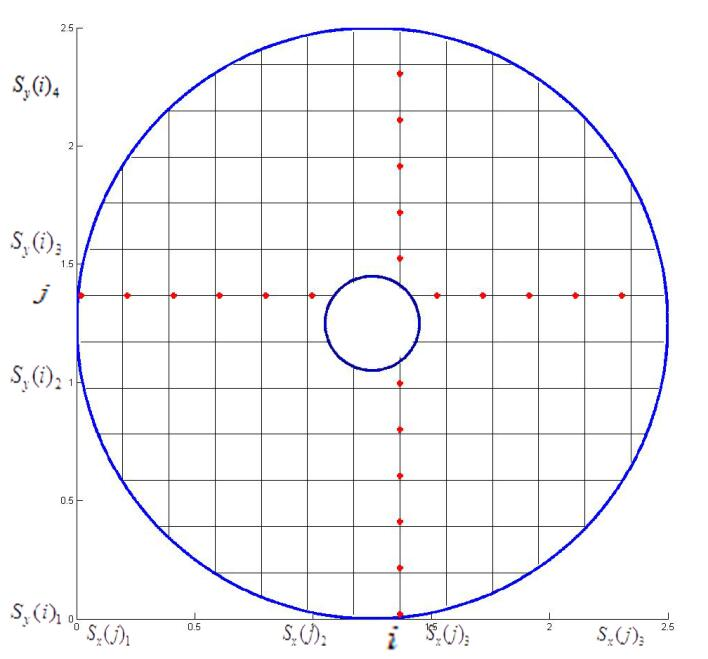
\includegraphics[width=0.6\textwidth,height=0.6\textwidth]{figures/Loop.jpg}
	\hspace{0.6\textwidth}
	\caption{多连通区域有限差分格式计算示意图}
	\label{FCR} 
\end{figure}



\section{矩阵预处理方法}
回火Riesz分数阶偏微分方程有限差分格式最终会转化为矩阵方程$A\bm{x}=\bm{b}$进行计算。由于实际问题中计算区域一般比较复杂并且分数阶导数具有非局部特性,导致系数矩阵的阶数非常大,并且通常为稠密矩阵。应用传统计算方法计算这种大规模稠密矩阵方程组需要消耗巨大的计算成本,例如使用共轭梯度法等数值方法产生的计算量为$O({{n}^{3}})$。目前,已经有很多针对分数阶扩散方程的高效算法出现。本章尝试将有限差分格式转换为矩阵方程组并应用预处理共轭梯度法进行计算,达到提升计算效率的目的。

\subsection{Toeplitz矩阵的预处理方法}

本章以ADI有限差分格式(3-19)-(3-20)为例应用预处理方法进行计算。首先将有限差分格式转化为矩阵方程组:
\begin{equation}
\begin{split}
{{T}_{1}}\bm{u_{z}^{*}}=\bm{u_{z}^{n-1}}+\tau{\bm{f}_{z}}  \quad    (1\le z\le {{m}_{2}}-1)
\end{split}
\end{equation}
其中$\bm{u_{z}^{*}}={{(u_{1,z}^{*},u_{2,z}^{*},u_{3,z}^{*},\cdots,u_{{{m}_{1}}-1,z}^{*})}^{T}}$,$\bm{u_{z}^{n-1}}={{(u_{1,z}^{n-1},u_{2,z}^{n-1},u_{3,z}^{n-1},\cdots,u_{{{m}_{1}}-1,z}^{n-1})}^{T}}$,\\${{\bm{f}_{z}}}={{(f(u(_{1,z}^{n-1},{{x}_{1}},{{y}_{z}},{{t}_{n-1}}),{{x}_{1}},{{y}_{z}},{{t}_{n-1}}),\cdots,f(u(_{{{m}_{1}}-1,z}^{n-1},{{x}_{{{m}_{1}}-1}},{{y}_{z}},{{t}_{n-1}}),{{x}_{{{m}_{1}}-1}},{{y}_{z}},{{t}_{n-1}}))}^{T}}$,矩阵${{T}_{1}}={{({{t}_{k}})}_{({{m}_{1}}-1)\times ({{m}_{1}}-1)}}$定义为:
\begin{equation}
t_{k}=\left\{\begin{array}{ll}{\tau r_{1}\left(w_{0}^{\left(\alpha_{1}\right)}+w_{2}^{\left(\alpha_{2}\right)}\right)} & {k=+1,-1} \\ {1+2 \tau r_{1} w_{1}^{\left(\alpha_{1}\right)}} & {k=0} \\ {\tau r_{1} w_{k+1}^{\left(\alpha_{1}\right)}} & {k>1} \\ {\tau r_{1} w_{1-k}^{\left(\alpha_{1}\right)}} & {k<-1}\end{array}\right.
\end{equation}
及方程组:
\begin{equation}
{{T}_{2}}\bm{\bar{u}_{l}^{n}}=\bm{\bar{u}_{l}^{*}} \quad  (1\le l\le {{m}_{1}}-1)
\end{equation}
其中$\bar{\bm{u}}_{l}^{*}={{(u_{l,1}^{*},u_{l,2}^{*},u_{l,3}^{*},\cdots ,u_{l,{{m}_{2}}-1}^{*})}^{T}}$,$\bar{\bm{u}}_{l}^{n}={{(u_{l,1}^{n},u_{l,2}^{n},u_{l,3}^{n},\cdots ,u_{l,{{m}_{2}}-1}^{n})}^{T}}$。矩阵${{T}_{2}}={{({{\tilde{t}}_{k}})}_{({{m}_{2}}-1)\times ({{m}_{2}}-1)}}$定义为:
\begin{equation}
\tilde{t}_{k}=\left\{\begin{array}{ll}{\tau r_{2}\left(w_{0}^{\left(\alpha_{2}\right)}+w_{2}^{\left(\alpha_{2}\right)}\right)} & {k=+1,-1} \\ {1+2 \tau r_{2} w_{1}^{\left(\alpha_{2}\right)}} & {k=0} \\ {\tau r_{2} w_{k+1}^{\left(\alpha_{2}\right)}} & {k>1} \\ {\tau r_{2} w_{1-k}^{\left(\alpha_{2}\right)}} & {k<-1}\end{array}\right.
\end{equation}

如上所示,矩阵$T_{1}$、$T_{2}$为Toeplitz矩阵,假设原Hermite-Toeplitz系统记为${{T}_{n}}x=\bm{b}$,其中矩阵$T_{n}=(t_{i,j})_{n}$的元素的定义为${{t}_{i,j}}={{t}_{i-j}}$。为了加快线性系统算法的收敛速度,需要对于原线性系统进行预处理。定义新的预处理后的线性系统为${{\tilde{T}}_{n}}\bm{\tilde{x}}=\bm{\tilde{b}}$,其中:${{\tilde{T}}_{n}}=C_{n}^{-1/2}{{T}_{n}}C_{n}^{-1/2}$,$\bm{\tilde{x}}=C_{n}^{1/2}\bm{x},\bm{\tilde{b}}=C_{n}^{-1/2}\bm{b}$ ,其中Hermit正定矩阵$C_{n}$ 为所需构造的预处理矩阵,其需要保证新构造的矩阵${{\tilde{T}}_{n}}$的谱是聚集的或者${{\tilde{T}}_{n}}$相较于${{T}_{n}}$良态\upcite{chan2007introduction}。随后若使用共轭梯度法(CG)求解预处理线性系统${{\tilde{T}}_{n}}\bm{\tilde{x}}=\bm{\tilde{b}}$,其主要的计算量来自于矩阵于向量的乘积$M_{n}^{-1}{{T}_{n}}\bm{v}$,其中$\bm{v}$为特定向量\upcite{golub1996cf,jin2006numerical,saad2003iterative}。Strang\upcite{strang1986proposal}与Olkin\upcite{olkin1986linear},对于任意Toeplitz矩阵${{T}_{n}}$构造循环矩阵${{C}_{n}}$作为预处理矩阵,可以提高计算矩阵向量乘$C_{n}^{-1}{{T}_{n}}\bm{v}$计算效率,计算量仅为$O(n\log n)$。本文应用R.Chan的循环预处理矩阵${{C}_{F}}({{T}_{n}})\text{=(}{{\text{c}}_{k}}{{)}_{n\times n}}$构造如下\upcite{chan1995best}:
\begin{equation}
c_{k}=\left\{\begin{array}{ll}{\frac{(n-k) t_{k}+k t_{k-n}}{n}} & {0 \leq k \leq n-1} \\ {c_{n+k}} & {0 \leq-k \leq n-1}\end{array}\right.
\end{equation}
综上所述,设计预处理共轭梯度法如下。

\begin{algorithm}
	\caption{预处理共轭梯度法}      %标题
	\begin{algorithmic} %每行显示行号
		\renewcommand{\algorithmicrequire}{\textbf{Input:}}
		\renewcommand{\algorithmicensure}{\textbf{Output:}}
	
		\REQUIRE Toeplitz矩阵${{T}_{n}}$,右端项$\bm{b}$,单步计算精度$tol$,最大迭代步数$Item$。    %输入
		\ENSURE $\bm{x}=\bm{{{z}_{k}}}{{c}_{F}}{{({{T}_{n}})}^{-1/2}}$                    %输出
		\	
		\begin{enumerate}[Step 1:]
			\item 将Toeplitz矩阵${{T}_{n}}$带入式(3-28)计算循环预处理矩阵${{C}_{F}}({{T}_{n}})$。
			\item 计算${{\tilde{T}}_{n}}={{C}_{F}}{{({{T}_{n}})}^{1/2}}{{T}_{n}}{{C}_{F}}{{({{T}_{n}})}^{-1/2}}$,$\bm{\tilde{b}}={{C}_{F}}{{({{T}_{n}})}^{-1/2}}\bm{b}$ ,$\bm{\tilde{x}}={{C}_{F}}{{({{T}_{n}})}^{1/2}}\bm{x}$ 构造新的线性系统${{\tilde{T}}_{n}}\bm{\tilde{x}}=\bm{\tilde{b}}$。
			\item
			任意给定初始向量$\bm{{\tilde{x}}_{0}}$,置$k=1$,计算$\bm{{r}_{1}}=\bm{\tilde{b}}-{{\tilde{T}}_{n}}\bm{{\tilde{x}}_{0}},\bm{{z}_{1}}=\bm{{r}_{1}}$。
			\item
			若$\bm{{r}_{k}}\le tol$或$\left< {{{\tilde{T}}}_{n}}\bm{{z}_{k}},\bm{{z}_{k}} \right>\le tol$终止计算,否则计算$\bm{{\tilde{x}}_{k+1}}=\bm{{\tilde{x}}_{k}}+\frac{\left<\bm{{r}_{k}},\bm{{z}_{k}}\right>}{\left<{{{\tilde{T}}}_{n}}\bm{{z}_{k}},\bm{{z}_{k}}\right>}\bm{{z}_{k}}$。
			\item
			计算$\bm{{r}_{k+1}}=\bm{\tilde{b}}-{{\tilde{T}}_{n}}\bm{{\tilde{x}}_{\text{k+1}}}$,$\bm{{z}_{k+1}}=\bm{{r}_{k+1}}-\frac{\left<\bm{{r}_{k+1}},{{{\tilde{T}}}_{n}}\bm{{z}_{k}}\right>}{\left<\bm{{z}_{k}},{{{\tilde{T}}}_{n}}\bm{{z}_{k}}\right>}\bm{{z}_{k}}=\bm{{r}_{k+1}}+\frac{{{\left\| \bm{{r}_{k+1}} \right\|}^{2}_{\infty}}}{{{\left\| \bm{{r}_{k}} \right\|}^{2}}_{\infty}}\bm{{z}_{k}}$。
			\item
			若$k=Item$时结束计算,否则置$k=k+1$,转Steps4。	
		\end{enumerate}		
	\end{algorithmic}
\end{algorithm}


\subsection{BTTB矩阵的预处理方法}
\noindent

更进一步,结合线性系统(3-24)-(3-27)将有限差分格式(3-18)转换为矩阵方程组
\begin{equation}
SH{\bm{u}^{n}}=\bm{b}
\end{equation}
其中矩阵$S$、$H$分别对应算子$(1+\tau r_{1} {{\theta }_{x}})$与$(1+\tau r_{2} {{\theta }_{y}})$ ,$\bm{b}$为矩阵$\bm{{\bm{u}}^{n-1}}+\tau \bm{{\bm{f}}^{n-1}}$按列遍历组成的向量,定义${{\bm{u}}^{n}}={{(u_{1,1}^{n},u_{2,1}^{n},\cdots u_{{{m}_{1}}-1,1}^{n},\cdots ,u_{1,{{m}_{2}}-1}^{n},\cdots u_{{{m}_{1}}-1,{{m}_{2}}-1}^{n})}^{T}}$,\\
$\bm{{\bm{f}}^{n}}={{(f_{1,1}^{n},f_{2,1}^{n},\cdots f_{{{m}_{1}}-1,1}^{n},\cdots ,f_{1,{{m}_{2}}-1}^{n},\cdots f_{{{m}_{1}}-1,{{m}_{2}}-1}^{n})}^{T}}$。
$S=diag({{T}_{1}},{{T}_{1}},\cdots ,{{T}_{1}})$为$({{m}_{1}}-1)\times({{m}_{2}}-1)$阶分块对角矩阵,而$H=(T_{2}^{(i,j)})$由$({{m}_{2}}-1)\times({{m}_{2}}-1)$个矩阵块组成,其中矩阵块$T_{2}^{(i,j)}=diag({{\tilde{t}}_{i-j}},{{\tilde{t}}_{i-j}},\cdots {{\tilde{t}}_{i-j}})$为$({{m}_{1}}-1)\times({{m}_{1}}-1)$阶矩阵。
新的线性系统(3-36)左端矩阵可写成如下形式:

\begin{equation}
\begin{split}
\tilde{A}&=SH=\left( \begin{matrix}
{{T}_{1}}T_{2}^{(1,1)} & {{T}_{1}}T_{2}^{(1,2)} & \cdots  & {{T}_{1}}T_{2}^{(1,{{m}_{2}}-1)}  \\
{{T}_{1}}T_{2}^{(2,1)} & {{T}_{1}}T_{2}^{(2,2)} & \cdots  & {{T}_{1}}T_{2}^{(2,{{m}_{2}}-1)}  \\
\vdots  & \vdots  & \vdots  & \vdots   \\
{{T}_{1}}T_{2}^{({{m}_{2}}-1,1)} & {{T}_{1}}T_{2}^{(.{{m}_{2}}-1,2)} & \cdots  & {{T}_{1}}T_{2}^{({{m}_{2}}-1,{{m}_{2}}-1)}  \\
\end{matrix} \right) \\
& =\left( \begin{matrix}
{{{\tilde{t}}}_{0}}{{T}_{1}} & {{{\tilde{t}}}_{-1}}{{T}_{1}} & \cdots  & {{{\tilde{t}}}_{-{{m}_{2}}}}{{T}_{1}}  \\
{{{\tilde{t}}}_{1}}{{T}_{1}} & {{{\tilde{t}}}_{0}}{{T}_{1}} & \cdots  & {{{\tilde{t}}}_{1-{{m}_{2}}}}{{T}_{1}}  \\
\vdots  & \vdots  & \vdots  & \vdots   \\
{{{\tilde{t}}}_{{{m}_{2}}-2}}{{T}_{1}} & {{{\tilde{t}}}_{{{m}_{2}}-3}}{{T}_{1}} & \cdots  & {{{\tilde{t}}}_{0}}{{T}_{1}}  \\
\end{matrix} \right)={{T}_{2}}\otimes {{T}_{1}} \\
\end{split}
\end{equation}
可以看出,$\tilde{A}$由$({{m}_{2}}-1)\times({{m}_{2}}-1)$个分块矩阵组成,其中矩阵块大小为$({{m}_{1}}-1)\times({{m}_{1}}-1)$。因为${{T}_{1}}$,${{T}_{2}}$均为Toeplitz矩阵,则易证各个矩阵块${{\tilde{t}}_{i-j}}{{T}_{1}}$为Toeplitz矩阵,同时$\tilde{A}$关于各个矩阵块构成Toeplitz矩阵,由此构成的矩阵我们命名为BTTB矩阵。

上一节介绍了针对Toeplitz矩阵所构造的线性系统系数矩阵应用R.Chan循环预处理方法进行高效计算。而对于式(3-30)所产生所产生的BTTB矩阵构成的线性系统,目前还没有找到较为高效的预处理方法聚合矩阵的谱。比较朴素的想法是对于各个Toeplitz矩阵块分别进行预处理,假设对于Toeplitz矩阵进行预处理算子记为${{c}_{U}}$,而对于BTTB矩阵的预处理算子记为$c_{U}^{(b)}$。若BTTB矩阵${{T}_{mn}}\in {{C}^{mn\times mn}}$定义为如下形式:
\[{{T}_{mn}}=\left( \begin{matrix}
{{A}_{0}} & {{A}_{-1}} & \cdots  & {{A}_{1-m}}  \\
{{A}_{1}} & {{A}_{0}} & \cdots  & {{A}_{2-m}}  \\
\vdots  & \vdots  & \vdots  & \vdots   \\
{{A}_{m-1}} & {{A}_{m-2}} & \cdots  & {{A}_{0}}  \\
\end{matrix} \right)\]
其中各个矩阵块${{A}_{i-j}}\in {{C}^{n\times n}}$。定义对BTTB预处理矩阵如下形式:
\[c_{U}^{\left( b \right)}({{T}_{mn}})=\left( \begin{matrix}
{{c}_{U}}({{A}_{0}}) & {{c}_{U}}({{A}_{-1}}) & \cdots  & {{c}_{U}}({{A}_{1-m}})  \\
{{c}_{U}}({{A}_{1}}) & {{c}_{U}}({{A}_{0}}) & \cdots  & {{c}_{U}}({{A}_{2-m}})  \\
\vdots  & \vdots  & \vdots  & \vdots   \\
{{c}_{U}}({{A}_{m-1}}) & {{c}_{U}}({{A}_{m-2}}) & \cdots  & {{c}_{U}}({{A}_{0}})  \\
\end{matrix} \right)\]

可以证明,应用这种方式定义的预处理矩阵处理后新的矩阵的谱更加集中\upcite{chan1992family},所以证明块算子预处理方法能够加快求解方程的迭代速度。经过分析,针对BTTB矩阵的预处理共轭梯度法计算复杂度为$O(mn{{\log }^{2}}(mn)+mn\log (mn))$,该方法产生的计算量远高于针对Toeplitz矩阵的预处理共轭梯度法,但相较于CG计算效率大幅度提高。随后将通过数值算例对比两种算法的实际计算效率。

\section{本章小结}
回火分数阶FHN模型由一个空间带有回火Riesz分数阶导数偏微分方程与整数阶常微分方程耦合而成,本章主要对于回火Riesz分数阶耦合系统建立有限差分格式进行计算。此外,为了降低高维情况下有限差分格式的计算复杂度,本文针对分数阶偏微分方程有限差分格式应用隐式交替方向方法进行处理。

为了在不规则区域上应用有限差分方法计算方程,首先结合Liu的思想\upcite{liu2015semi}及G-L分数阶导数定义对于有限差分格式(3-10)及初边值离散条件(3-14)、(3-16)进行修改,使其适应在单连通不规则区域上进行计算。由于多联通不规则区域的复杂性,并不能直接应用有限差分格式进行计算,算法1将多联通不规则区域划分为多个单连通子区域进行计算,使得离散格式计算具有普适性。

随后,本章将有限差分格式转换为矩阵方程。受到分数阶导数非局部特性及复杂的计算区域的影响,有限差分格式产生的线性系统的矩阵通常为大规模稠密矩阵,应用传统算法计算效率甚低,本章结合R.Chan构造的循环预处理方法对于针对Toeplitz矩阵系统及BTTB矩阵系统进行处理,构造预处理共轭梯度法对于矩阵方程进行求解,以期提高计算效率。

\clearpage


\chapter{数值实验}
本章设计数值算例主要分为四部分:1、对于有限差分格式的收敛阶的计算;2、应用有限差分格式在方形区域、圆形区域、环形区域及心脏横向不规则区域上计算回火分数阶FHN模型;3、应用预处理共轭梯度法计算模型并验证算法计算效果;4、探究回火分数阶导数对于计算结果的影响。
 \section{有限差分格式收敛阶的计算}
本文应用有限差分方法计算带有回火Riesz分数阶导数的耦合系统方程,并对系统的收敛性及稳定性进行了分析。本节通过应用有限差分格式计算回火Riesz分数阶扩散方程,验证有限差分格式的收敛阶。\\
\textbf{例1}:为了验证有限差分格式数值精度,考虑空间Riesz分数阶导数扩散方程:
\[
\frac{\partial u}{\partial t}=\frac{\partial^{(\alpha, \lambda)} u}{\partial|x|^{(\alpha, \lambda)}}+f(x, t)
\]
其中$(x,t)\in [0,1]\times (0,1]$,初值条件为$u(x,0)=x^{3}\left(1-x\right)^{3}$,边界条件为$u(0,t)=u(1,t)=0\quad t\in [0,1]$ ,当回火指数$\lambda = 0$,上述扩散方程存在精确解$u(x, t)=e^{-t}x^{3}\left(1-x\right)^{3}$。
定义源项函数为:
\[
\begin{aligned}
f(x, t)=-\mathrm{e}^{-t}\left(x^{3}(1-x)^{3}+\frac{\Gamma(4)}{\Gamma(4-\alpha)}\left(x^{3}+(1-x)^{3}\right)-3 \frac{\Gamma(5)}{\Gamma(5-\alpha)}\left(x^{4}+(1-x)^{4}\right)\right.\\
\left.+3 \frac{\Gamma(6)}{\Gamma(6-\alpha)}\left(x^{5}+(1-x)^{5}\right)-\frac{\Gamma(7)}{\Gamma(7-\alpha)}\left(x^{6}+(1-x)^{6}\right)\right)
\end{aligned}
\]
本文使用无穷范数$\|\cdot\|_{\infty}$来计算数值格式的空间收敛阶,空间与时间方向上的收敛阶定义如下:
\begin{align*}
\text {order}=\left\{\begin{array}{ll}{\frac{\log \left(\left\|\eta\left(\tau_{1}, N, t_{n}\right)\right\|_{\infty}  /\left\|\eta\left(\tau_{2}, N, t_{n}\right)\right\|_{\infty} \right)}{\log \left(\tau_{1} / \tau_{2}\right)},} & {\text { 时间方向 }} \\
{\frac{\log \left(\left\|\eta\left(\tau, N_{1}, t_{n}\right)\right\|_{\infty}  /\left\|\eta\left(\tau, N_{2}, t_{n}\right)\right\|_{\infty} \right)}{\log \left(N_{1} / N_{2}\right)},} & {\text { 空间方向 }}\end{array}\right.
\end{align*}
其中$\eta\left(\tau, N, t_{n}\right)$表示在空间网格节点为$N$,时间步长为$\tau$,在$t=t_{n}$条件下数值解与对应的精确解的数值误差。设置$\alpha $分别为1.7、1.9。时间步长设为$\tau=h^{2}$ ,应用有限差分格式(3-11)计算在$T=1$时刻产生的误差及收敛阶。

\begin{table*}[h]
	\centering
	%	\captiontitlefont{\xiaowuhao\bf }
	% \captionsetup{font={small}}
	\caption[labelTabtab1]{$\alpha=1.7$条件下Euler差分格式计算的数值误差与收敛阶}
	\renewcommand\tabcolsep{0.5em}
	% \xiaowuhao \selectfont
	% \renewcommand{\arraystretch}{0.8}
	% \fontsize{9}{11}\selectfont
	\label{tab:feat_combin}
	\begin{tabular}{|c|c|c|c|c|}
		\hline
	
		{Alpha}&{N} &$\| u-u_h\|_{\infty}$  & order(space) & order(time) \cr
		%	\begin{tabular}{cc|ccccc}
		%		\toprule {Alpha} & {N} &  {$\lambda =0$  } & {$\lambda =0.1$  } & {$\lambda =1$  } & {$\lambda =10$  }\\
		\hline\hline
		\multirow{4}{*}{1.7} 
		& 32 & 8.8271e-04 & - & - \\
		& 64 & 2.6562e-04& 1.7326& 0.8663\\
		& 128 & 7.4429e-05& 1.8426&  0.9177 \\
		& 256 &  2.0586e-05&  1.8554 &   0.9277 \\
		
		\bottomrule
		\bottomrule
	\end{tabular}
\end{table*}

\begin{table*}[h]
	\centering
	%	\captiontitlefont{\xiaowuhao\bf }
	% \captionsetup{font={small}}
	\caption[labelTabtab1]{$\alpha=1.9$条件下Euler差分格式计算的数值误差与收敛阶}
	\renewcommand\tabcolsep{0.5em}
	% \xiaowuhao \selectfont
	% \renewcommand{\arraystretch}{0.8}
	% \fontsize{9}{11}\selectfont
	\label{tab:feat_combin}
	\begin{tabular}{|c|c|c|c|c|}
		\hline
		
		{Alpha}&{N} &$\| u-u_h\|_{\infty}$  & order(space) & order(time) \cr
		%	\begin{tabular}{cc|ccccc}
		%		\toprule {Alpha} & {N} &  {$\lambda =0$  } & {$\lambda =0.1$  } & {$\lambda =1$  } & {$\lambda =10$  }\\
		\hline\hline
		\multirow{4}{*}{1.9} 
		& 32 & 5.4838Ee-04 & - & - \\
		& 64 & 1.5400e-04&1.8322& 0.9161\\
		& 128 &  4.2027e-05& 1.8736&    0.9368 \\
		& 256 &  1.1105e-05&  1.9201 &  0.9601 \\
		
		\bottomrule
		\bottomrule
	\end{tabular}
\end{table*}
表(4-1)、(4-2)分别给出应用有限差分格式(3-11)计算空间带有Riesz分数阶导数的扩散方程在$T=1$时刻的数值误差及空间收敛阶。本例分别设置空间分数阶阶数为$\alpha =1.3$、$\alpha=1.8$。从计算结果可以看出,当空间步长与时间步长足够小时,有限差分格式所计算的数值解与精确解基本重合,这证明所建立的有限差分格式的有效性。此外,在无穷范数$\|\cdot\|_{\infty}$意义下计算的空间收敛阶趋近于2,时间方向收敛阶趋近于1,这与理论分析结果相符。此外,在不同分数阶阶数条件下计算的空间收敛阶均趋近于相同的结果,这证明分数阶阶数对于有限差分格式计算结果的数值精度影响不大。

%%%%%%%%%%%%%%%%%%%%%%%%%%%%%%%%%%%%%%%%%%%%%%%

\section{二维回火Riesz空间分数阶FHN模型}
\noindent   %当行不缩进
\textbf{例2}:考虑二维回火分数阶FHN模型
\[
\begin{split}
& \frac{\partial u}{\partial t}={{K}_{x}}\frac{{{\partial }^{({{\alpha }_{1}},{{\lambda }_{1}})}}u}{\partial {{\left| x \right|}^{({{\alpha }_{1}},{{\lambda }_{1}})}}}+{{K}_{y}}\frac{{{\partial }^{({{\alpha }_{2}},{{\lambda }_{2}})}}u}{\partial {{\left| y \right|}^{({{\alpha }_{2}},{{\lambda }_{2}})}}}+u(1-u)(u-\delta )-v \\
& \frac{\partial v}{\partial t}=\varepsilon (au-bv+c) \quad (x,y,t)\in \Omega \times (0,T] \\
\end{split}
\]	
其中$\Omega =[0,2.5]\times[0,2.5]$,$\delta =0.1$、$\varepsilon =0.01$、$a =0.5$、$b =1$、$c =0$。取初值为
\[u(x, y, 0)=\left\{\begin{array}{ll}{1.0,} & {0<x \leq 1.25,0<y<1.25} \\ {0.0,} & {1.25 \leq x<2.5,0<y<1.25} \\ {0.0,} & {0<x \leq 1.25,1.25 \leq y<2.5} \\ {0.0,} & {1.25 \leq x<2.5,1.25 \leq y<2.5}\end{array}\right.\]
\[v(x, y, 0)=\left\{\begin{array}{ll}{0.0,} & {0<x \leq 1.25,0<y<1.25} \\ {0.0,} & {1.25 \leq x<2.5,0<y<1.25} \\ {0.1,} & {0<x \leq 1.25,1.25 \leq y<2.5} \\ {0.1,} & {1.25 \leq x<2.5,1.25 \leq y<2.5}\end{array}\right.\]
边界条件为
\[
\begin{split}
& u\left( 0,y,t \right)=u\left( 2.5,y,t \right)=0 \\
& v\left( x,0,t \right)=v\left( x,2.5,t \right)=0 \\
\end{split}
\]

将空间区域$\Omega $划分成${{m}_{1}}\times {{m}_{2}}=256\times 256$的离散区域,时间步长$\tau =0.1$,终止时间设为$T=1000$。扩散方程应用有限差分格式(3-11)、(3-14)、(3-15)-(3-18),常微分方程应用向后Euler格式进行计算。为了验证数值格式计算效果,本例将与Liu的计算结果\upcite{liu2013numerical}进行对比。置$\lambda =0$,即原系统退化为标准分数阶FHN模型。设置扩散系数为${{K}_{x}}={{K}_{y}}={{10}^{-4}}$,分数阶阶数为${{\alpha }_{1}}={{\alpha }_{2}}=2.0$。计算终止时刻为$T=1000$条件下跨膜电势随时间的变化情况,结果如图(4-1)-图(4-4)所示。
\begin{figure}[htbp]
	\centering
	
	\subfigure[]
	{
		\begin{minipage}{7cm}
			\centering
			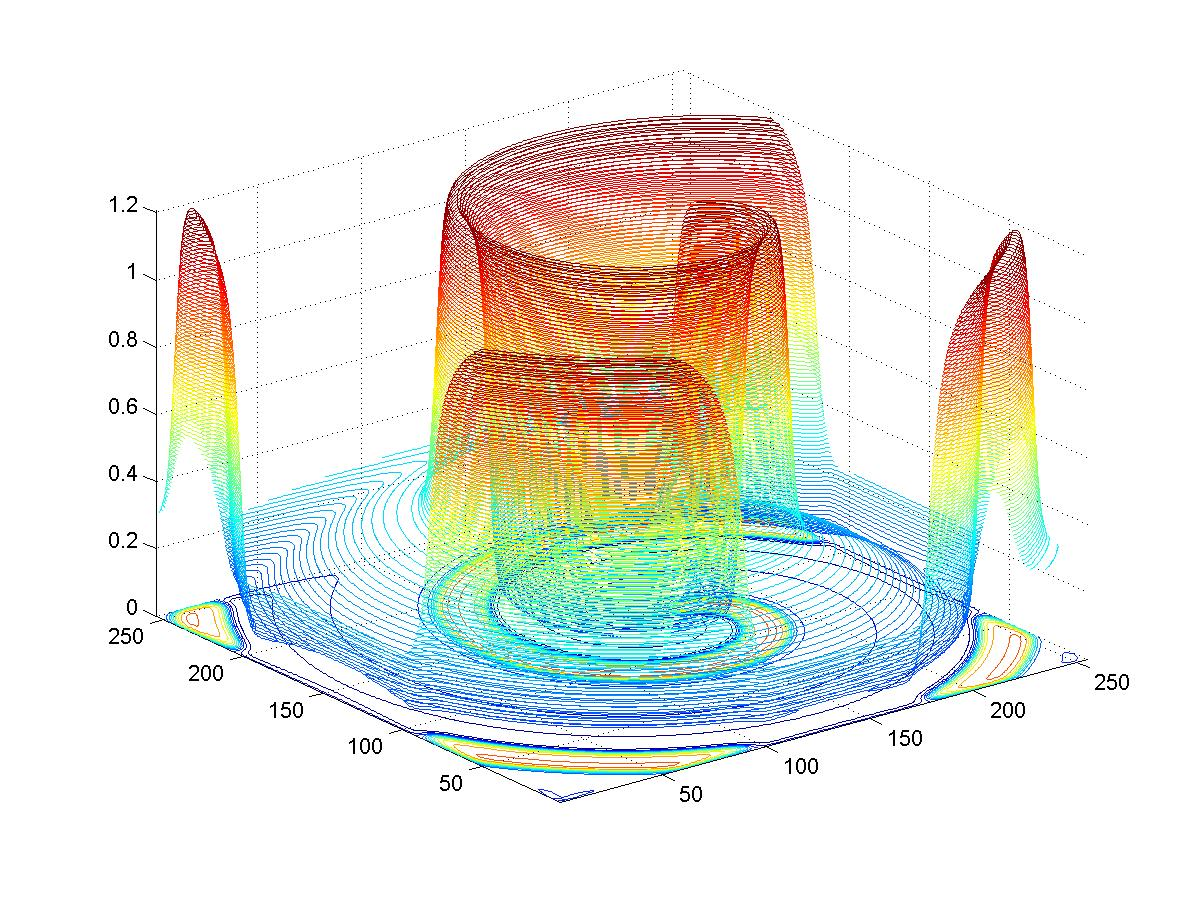
\includegraphics[width=5.5cm,height=5.5cm,scale=1]{figures/DLay50.jpg}
		\end{minipage}
	}
	\subfigure[]
	{
		\begin{minipage}{7cm}
			\centering
			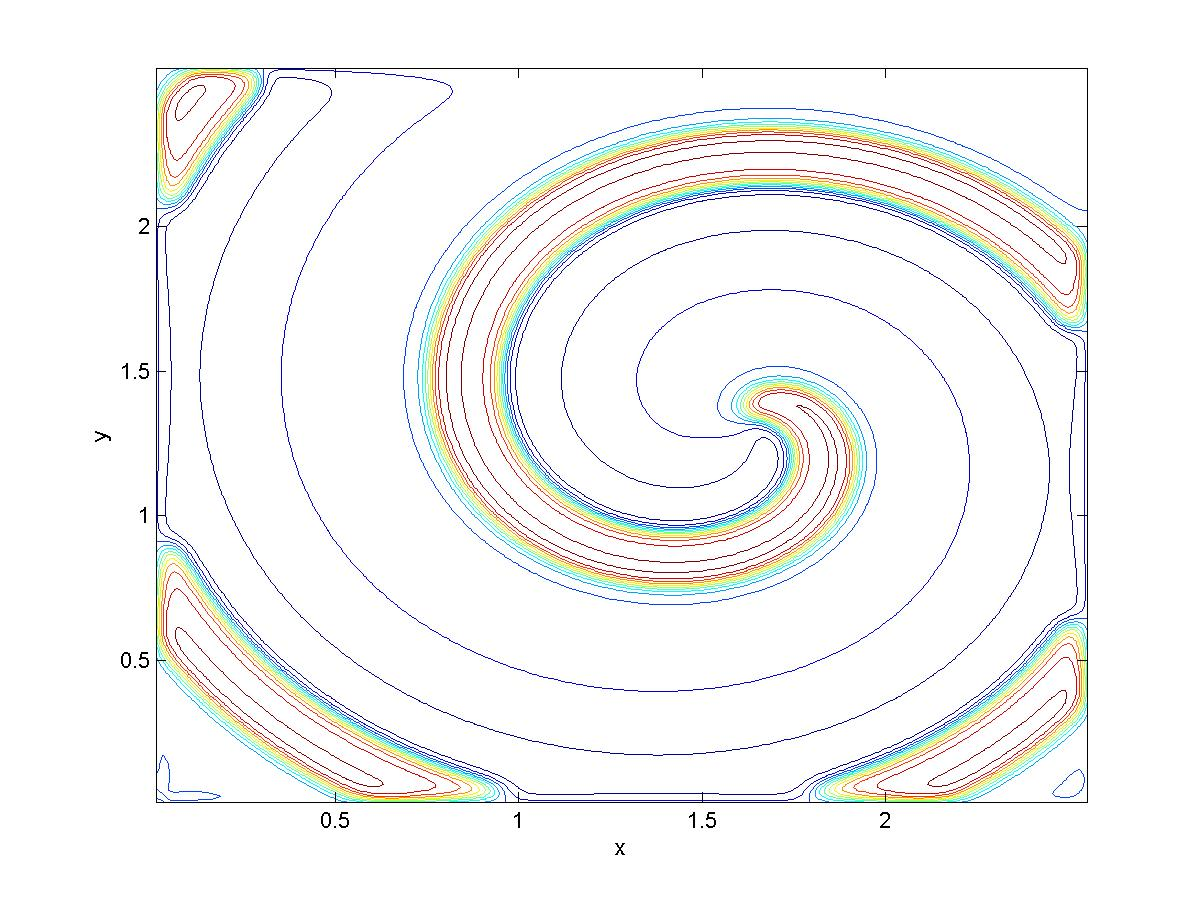
\includegraphics[width=5cm,height=5cm,scale=1]{figures/Lay50.jpg}
		\end{minipage}
	}
	
	
	\setlength{\abovecaptionskip}{-0.2cm} %调整图片标题与图距离 
	\caption{$\alpha = 2.0,K_{x} = K_{y} = {10}^{-4}$,跨膜电势$u$在$T=500$时刻对比图}
	\label{fig:1a}
	\vspace{-0.5cm} %设定値自由调整
	\subfigure[]
	{
		\begin{minipage}{7cm}
			\centering
			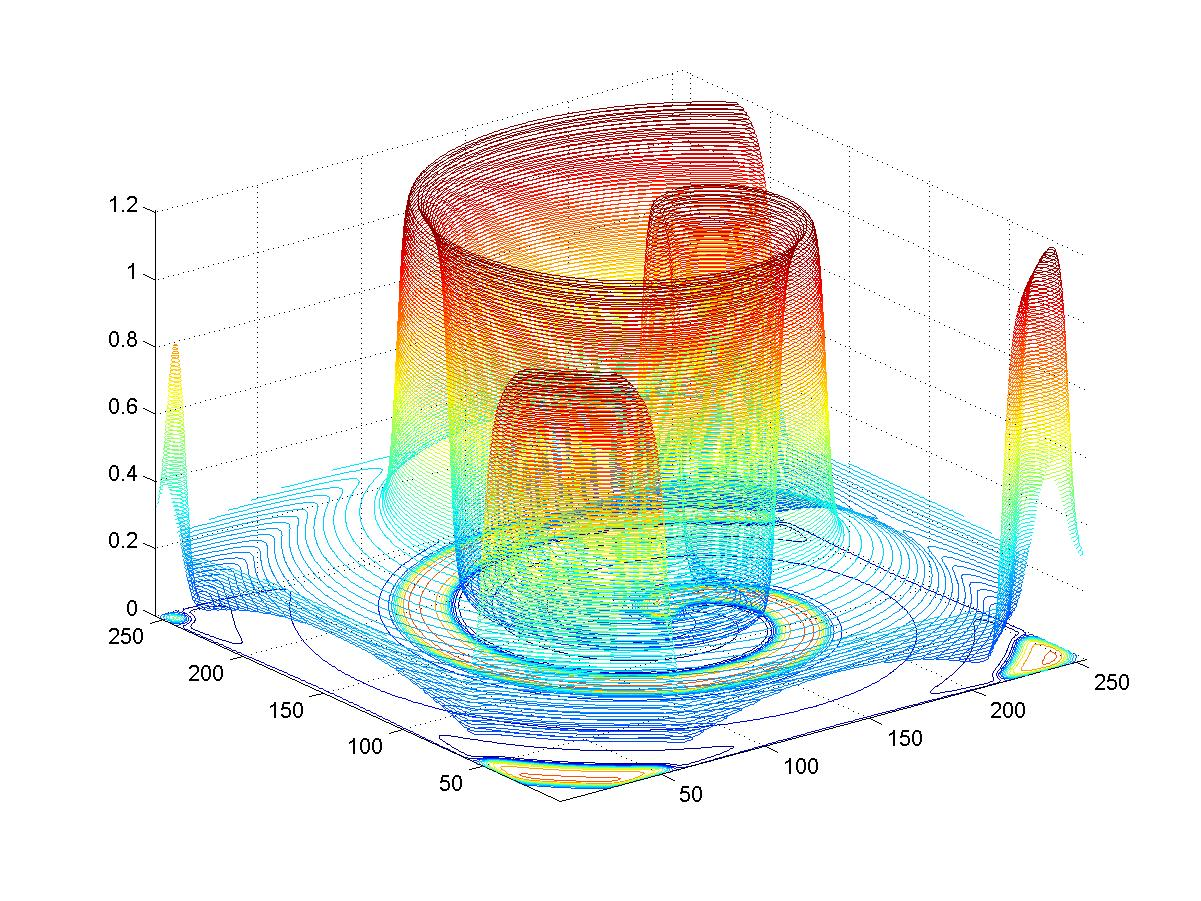
\includegraphics[width=5.5cm,height=5.5cm,scale=1]{figures/DLay53.jpg}
		\end{minipage}
	}
	\subfigure[]
	{
		\begin{minipage}{7cm}
			\centering
			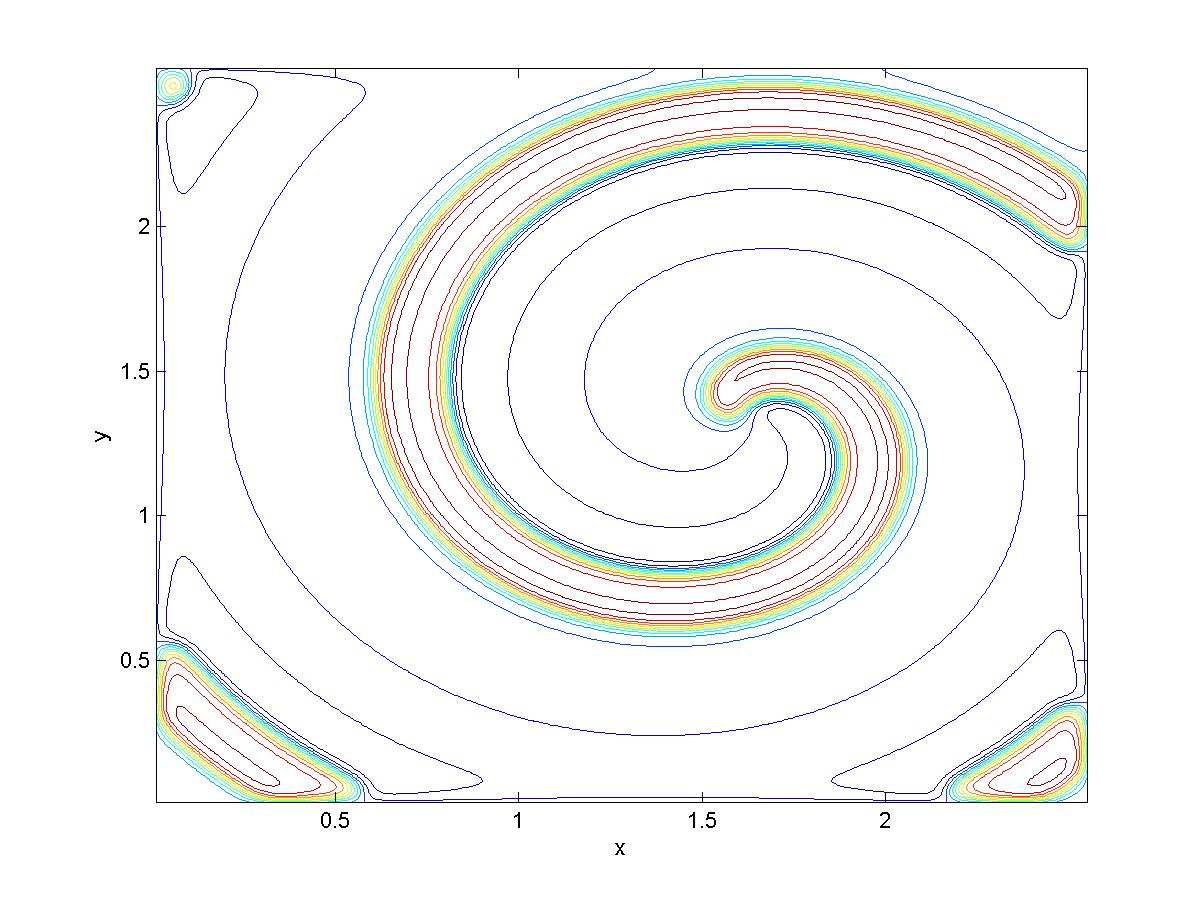
\includegraphics[width=5cm,height=5cm,scale=1]{figures/Lay53.jpg}
		\end{minipage}
	}
	
	\caption{$\alpha = 2.0,K_{x} = K_{y} = {10}^{-4}$,跨膜电势$u$在$T=530$时刻对比图}
	\label{fig:1b}
	\subfigure[]
	{
		\begin{minipage}{7cm}
			\centering
			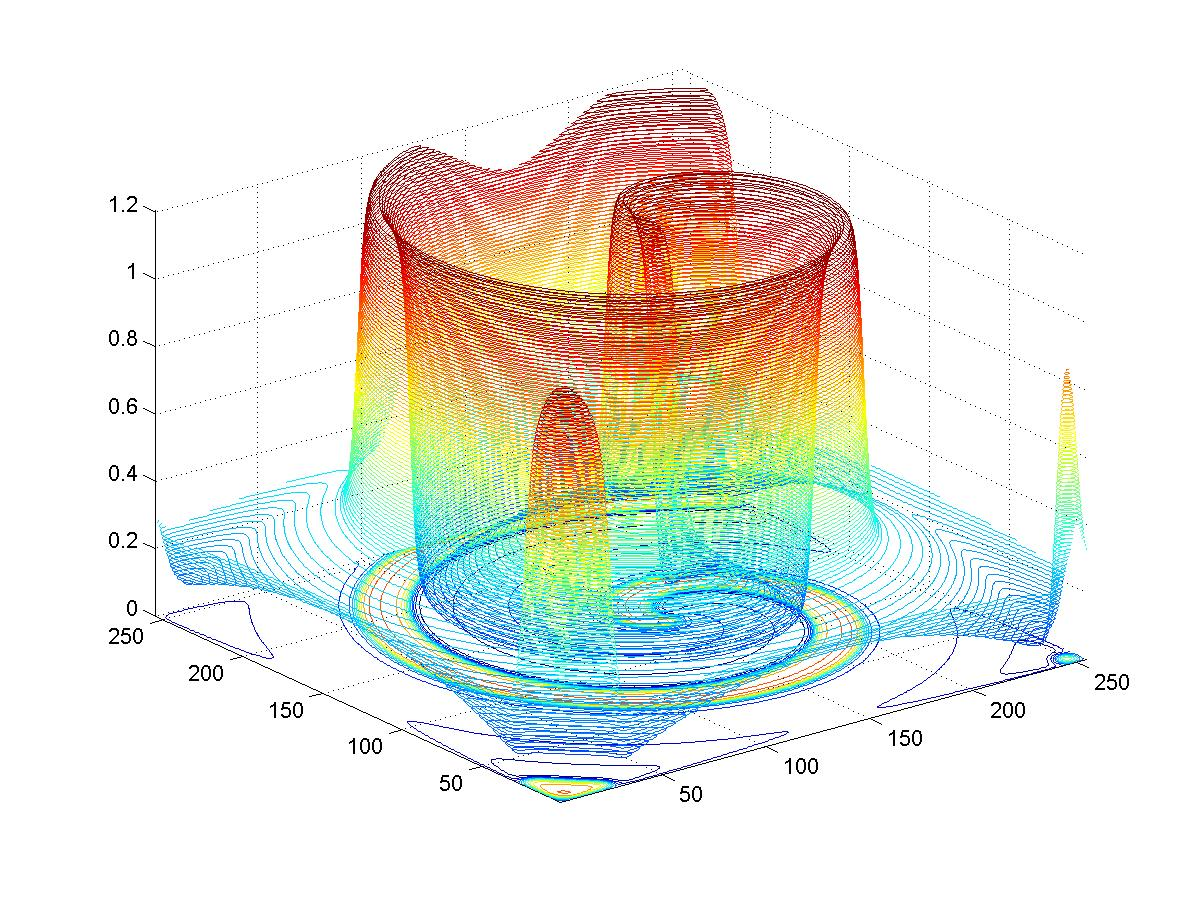
\includegraphics[width=5.5cm,height=5.5cm,scale=1]{figures/DLay56.jpg}
		\end{minipage}
	}
	\subfigure[]
	{
		\begin{minipage}{7cm}
			\centering
			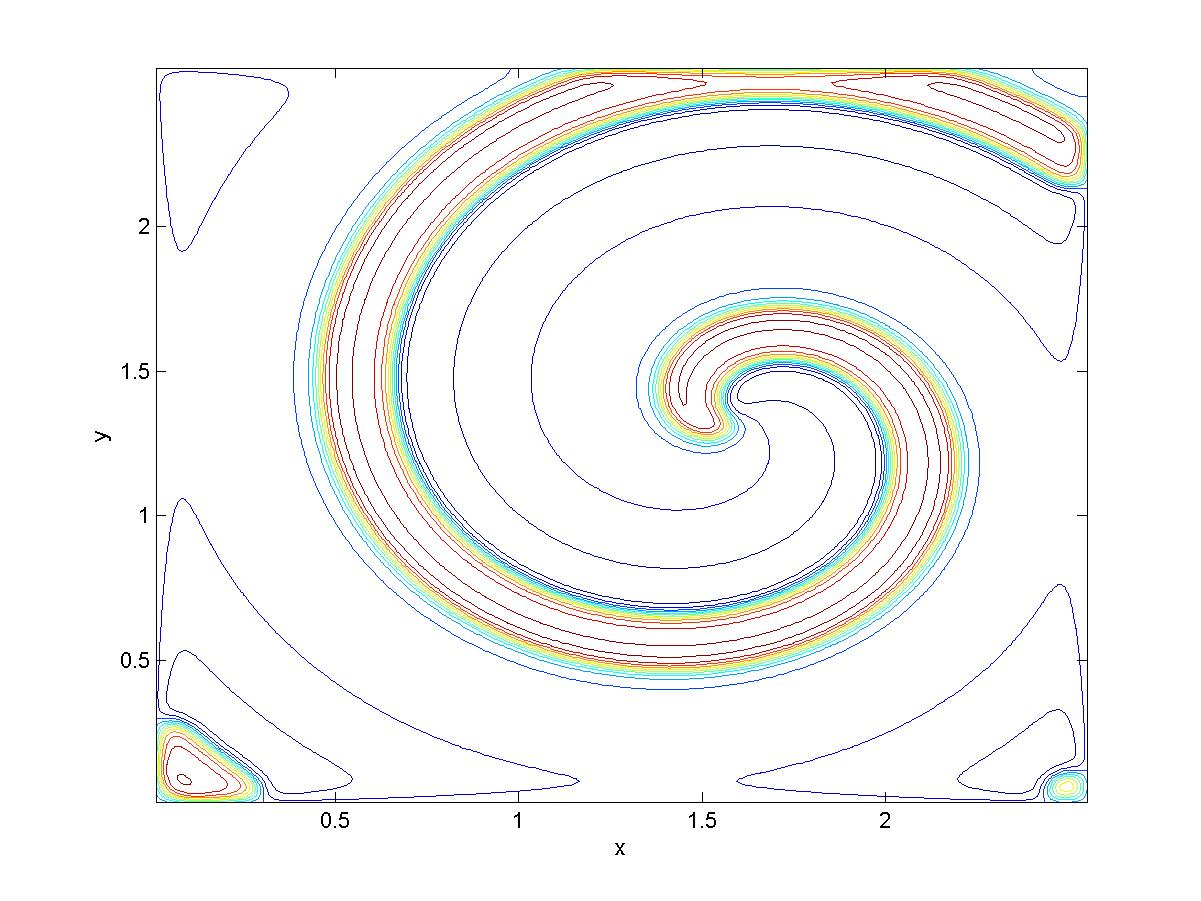
\includegraphics[width=5cm,height=5cm,scale=1]{figures/Lay56.jpg}
		\end{minipage}
	}
	\setlength{\abovecaptionskip}{-0.2cm} %调整图片标题与图距离 
	\caption{$\alpha = 2.0,K_{x} = K_{y} = {10}^{-4}$,跨膜电势$u$在$T=560$时刻对比图}
	\label{fig:1b}
	\vspace{-0.5cm} %设定値自由调整
	
	
	\subfigure[]
	{
		\begin{minipage}{7cm}
			\centering
			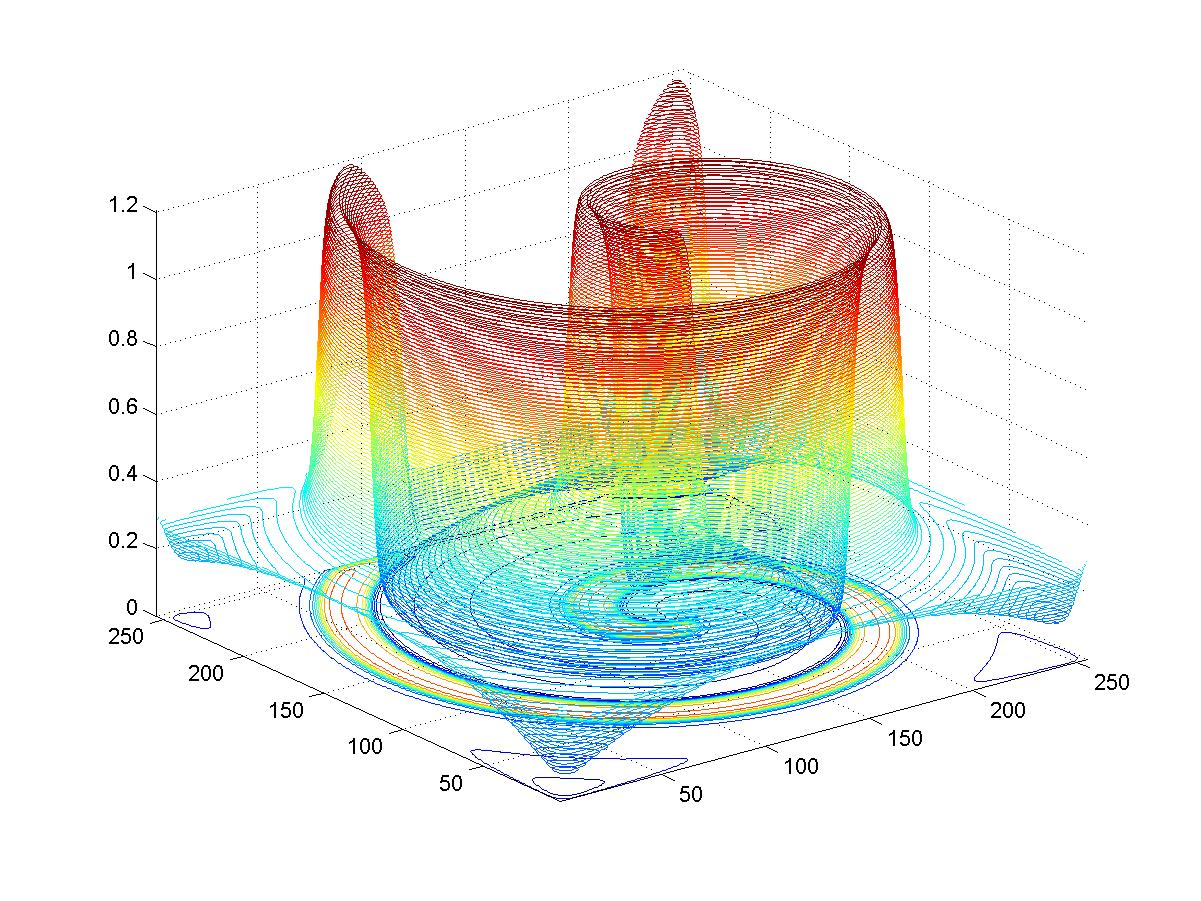
\includegraphics[width=5.5cm,height=5.5cm,scale=1]{figures/DLay59.jpg}
		\end{minipage}
	}
	\subfigure[]
	{
		\begin{minipage}{7cm}
			\centering
			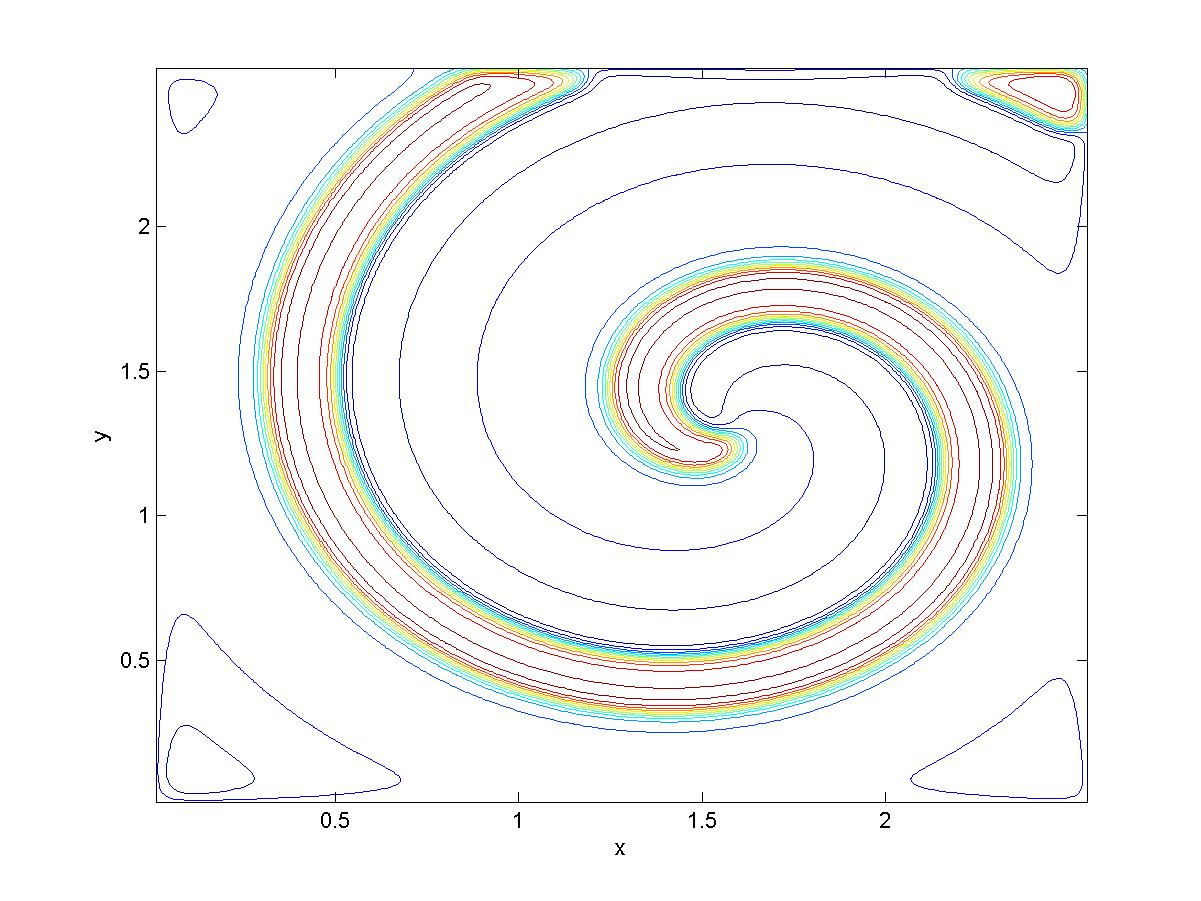
\includegraphics[width=5cm,height=5cm,scale=1]{figures/Lay59.jpg}
		\end{minipage}
	}
	\setlength{\abovecaptionskip}{-0.2cm} %调整图片标题与图距离 
	\caption{$\alpha = 2.0,K_{x} = K_{y} = {10}^{-4}$,跨膜电势$u$在$T=590$时刻对比图}
	\label{fig:1b}
	\vspace{-0.5cm} %设定値自由调整
		
\end{figure}

图(4-1)-图(4-4)分别呈现出跨膜电势$u$随着时间的变化情况,在方形扩散区域上跨膜电势$u$以螺旋波的形式向外传播。更进一步可以观察到,尽管受到初值条件的影响,电势传播形式总是最终转变为螺旋波,并且传播速度一定,并具有一定的周期性。随后将设计算例验证方程中各个参数对于螺旋波的影响。分别计算扩散系数为${{K}_{x}}={{K}_{y}}={{10}^{-4}}$,${{K}_{x}}={{K}_{y}}={{10}^{-5}}$,分数阶阶数为${{\alpha }_{1}}={{\alpha }_{2}}=2.0$及${{\alpha }_{1}}={{\alpha }_{2}}=1.7$时的计算结果。终止时刻$T=1000$下的数值计算结果如图(4-5)-图(4-8)所示。




\begin{figure}[htbp]
	\centering

	\subfigure[]
	{
		\begin{minipage}{6cm}
			\centering
			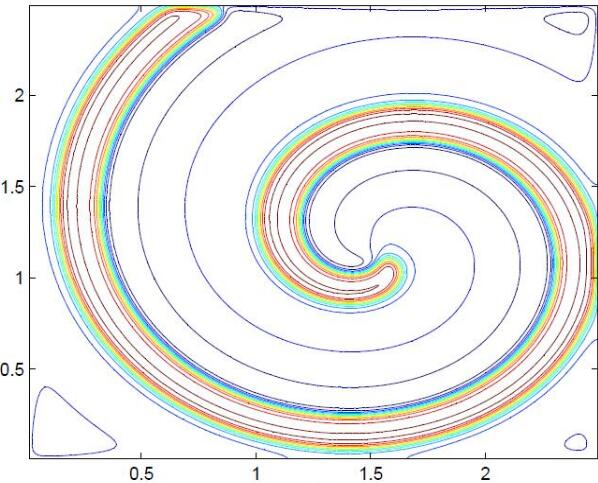
\includegraphics[width=4.5cm,height=4.5cm,scale=1]{figures/Alpha2.0_Kx_1e-4ofLiu.jpg}
		\end{minipage}
	}
	\subfigure[]
	{
		\begin{minipage}{6cm}
			\centering
			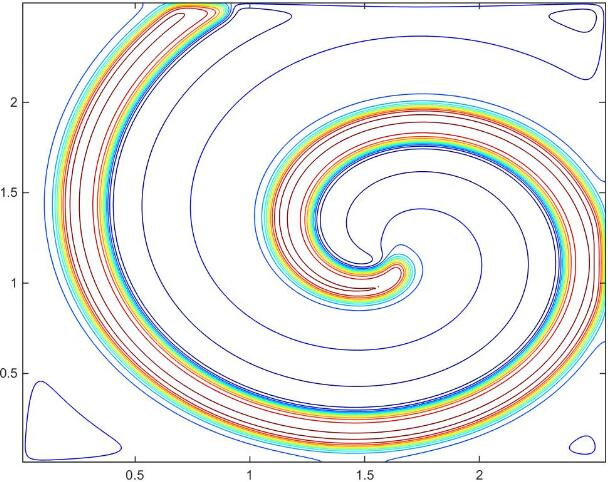
\includegraphics[width=4.5cm,height=4.5cm,scale=1]{figures/Alpha2.0_Kx_1e-4.jpg}
		\end{minipage}
	}
	\setlength{\abovecaptionskip}{-0.2cm} %调整图片标题与图距离 
	\caption{$\alpha = 2.0,K_{x} = K_{y} = {10}^{-4}$,跨膜电势$u$在$T=1000$时刻对比图}
	\label{fig:1a}
	\vspace{-0.5cm} %设定値自由调整 
	\subfigure[]
	{
		\begin{minipage}{6cm}
			\centering
			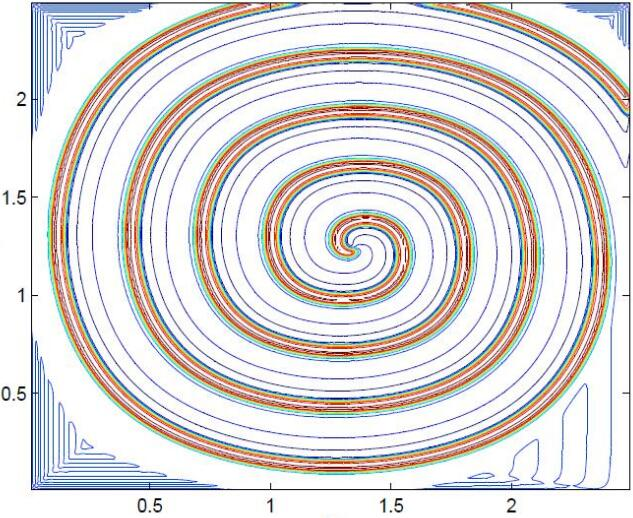
\includegraphics[width=4.5cm,height=4.5cm,scale=1]{figures/Alpha2.0_Kx_1e-5ofLiu.jpg}
		\end{minipage}
	}
	\subfigure[]
	{
		\begin{minipage}{6cm}
			\centering
			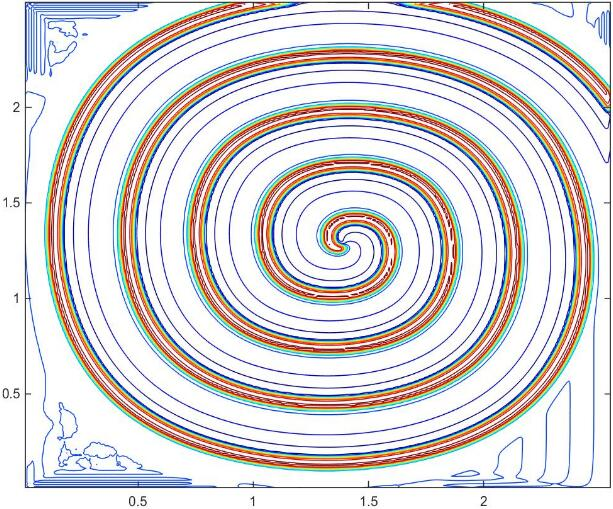
\includegraphics[width=4.5cm,height=4.5cm,scale=1]{figures/Alpha2.0_Kx_1e-5.jpg}
		\end{minipage}
	}
	\setlength{\abovecaptionskip}{-0.2cm} %调整图片标题与图距离 
	\caption{$\alpha = 2.0,K_{x} = K_{y} = {10}^{-5}$,跨膜电势$u$在$T=1000$时刻对比图}
	\label{fig:1b}
	\vspace{-0.5cm} %设定値自由调整

	\subfigure[]
	{
		\begin{minipage}{6cm}
			\centering
			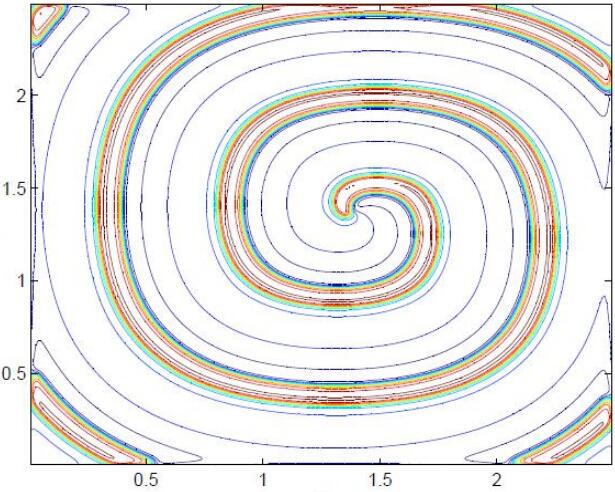
\includegraphics[width=4.5cm,height=4.5cm,scale=1]{figures/Alpha1.7_Kx_1e-4ofLiu.jpg}
		\end{minipage}
	}
	\subfigure[]
	{
		\begin{minipage}{6cm}
			\centering
			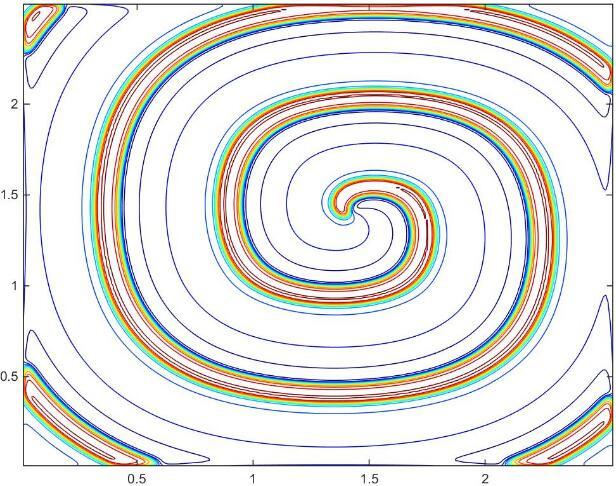
\includegraphics[width=4.5cm,height=4.5cm,scale=1]{figures/Alpha1.7_Kx_1e-4.jpg}
		\end{minipage}
	}

	\setlength{\abovecaptionskip}{-0.2cm} %调整图片标题与图距离 
	\caption{$\alpha = 1.7,K_{x} = K_{y} = {10}^{-4}$,跨膜电势$u$在$T=1000$时刻对比图}
	\label{fig:1c}
	\vspace{-0.5cm} %设定値自由调整
	
	\subfigure[]
	{
		\begin{minipage}{6cm}
			\centering
			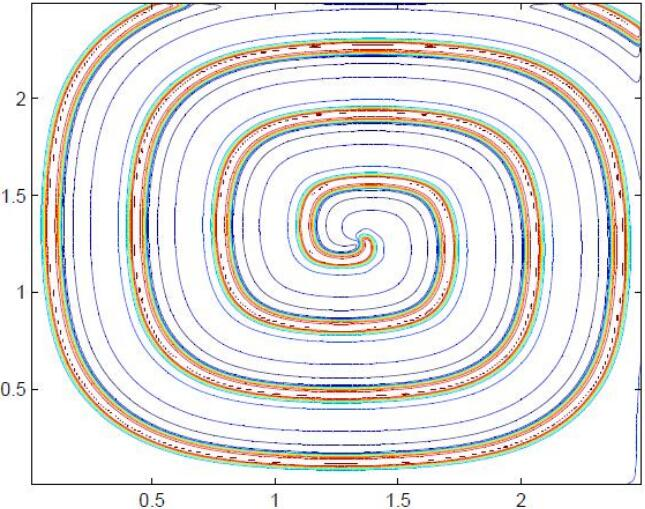
\includegraphics[width=4.5cm,height=4.5cm,scale=1]{figures/Alpha1.5_Kx_1e-4ofLiu.jpg}
		\end{minipage}
	}
	\subfigure[]
	{
		\begin{minipage}{6cm}
			\centering
			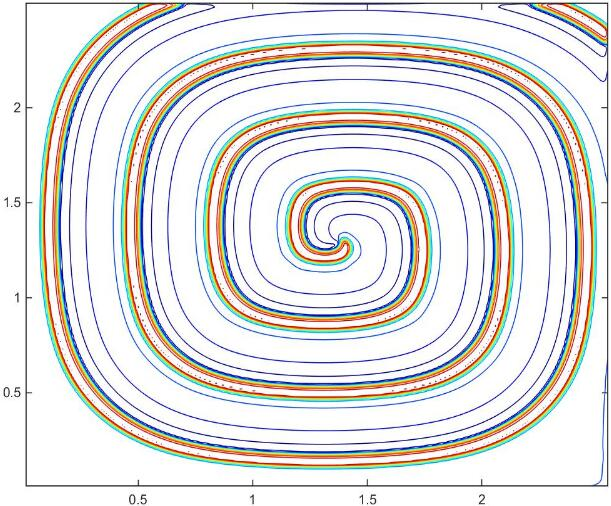
\includegraphics[width=4.5cm,height=4.5cm,scale=1]{figures/Alpha1.5_Kx_1e-4.jpg}
		\end{minipage}
	}
	\setlength{\abovecaptionskip}{-0.2cm} %调整图片标题与图距离 
	\caption{$\alpha = 1.5,K_{x} = K_{y} = {10}^{-4}$,跨膜电势$u$在$T=1000$时刻对比图}
	\label{fig:1d}
	\vspace{-0.5cm} %设定値自由调整

\end{figure}


从上图(4-5)-图(4-8)可以看出,当回火指数$\lambda=0$时,回火分数阶FHN模型完全退化为标准分数阶FHN模型。与Liu关于Riesz分数阶FHN模型的计算结果对比\upcite{liu2013numerical},在相同条件下计算结果基本一致,验证所构造的有限差分格式的有效性。更进一步,通过改变分数阶阶数及扩散系数验证分数阶微分方程中各项系数的改变对于计算结果的影响。通过下面的计算结果可以看出,矩形区域上跨膜电势$u$在初值条件的影响下,逐渐呈现出以螺旋波的形式自发而稳定地向外传播的效果。在相同扩散系数条件下,激发波前的宽度随着分数阶阶数的降低而明显减小。相同条件下,减小扩散系数可以得到与减小分数阶阶数一致的效果趋势,但是改变扩散系数与分数阶阶数对计算效果的影响并不等价。


更进一步,为了验证具有各向异性的扩散系数与分数阶阶数对于计算结果的影响,上述条件不发生改变,设置在分数阶为$\alpha_{1}=\alpha_{2}=2.0$,空间各向异性扩散系数比例为$K_{x}={10}^{-4}$,$K_{y}/K_{x}=0.25$及$K_{y}={10}^{-4}$,$K_{x}/K_{y}=0.25$,计算结果如图(4-5)-(4-6)所示。另一方面,扩散系数不发生变化,空间分数阶阶数分别比例设置为$\alpha_{1}=2$,$\alpha_{1}/\alpha_{2}=0.825$及$\alpha_{2}=2$,$\alpha_{2}/\alpha_{1}=0.825$时计算结果如图(4-7)-(4-8)所示。
\begin{figure}[htbp]
	\centering
	
	\subfigure[]
	{
		\begin{minipage}{6cm}
			\centering
			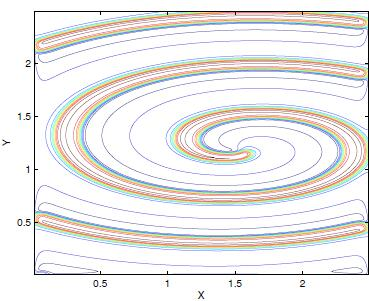
\includegraphics[width=4.5cm,height=4.5cm,scale=1]{figures/LiuKx=0.25Ky.jpg}
		\end{minipage}
	}
	\subfigure[]
	{
		\begin{minipage}{6cm}
			\centering
			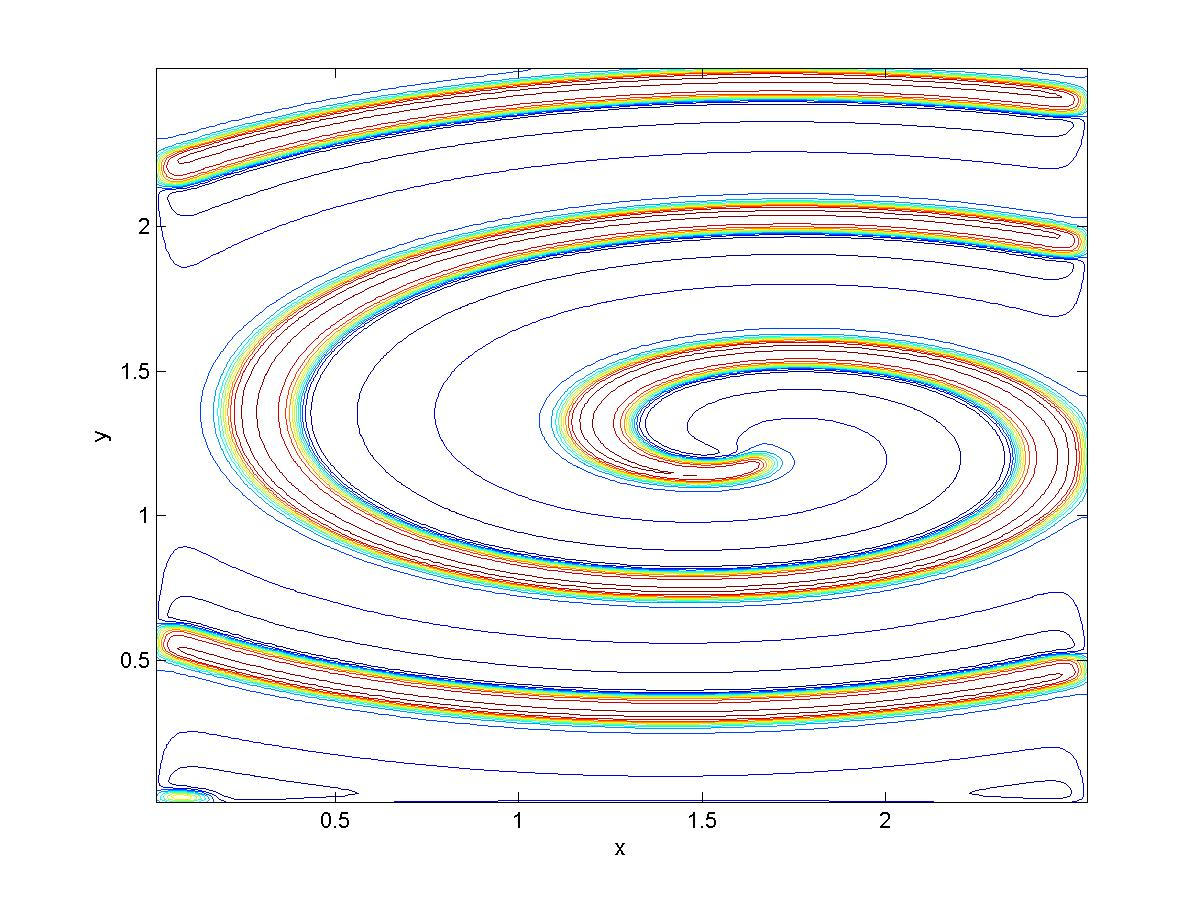
\includegraphics[width=5.1cm,height=5cm,scale=1]{figures/Kx=0.25Ky.jpg}
		\end{minipage}
	}
	\setlength{\abovecaptionskip}{-0.2cm} %调整图片标题与图距离 
	\caption{$K_{x}=10^{-4},K_{y}/K_{x} = 0.25$,跨膜电势$u$在$T=1000$时刻对比图}
	\label{fig:1a}
	\vspace{-0.5cm} %设定値自由调整
	
	\subfigure[]
	{
		\begin{minipage}{6cm}
			\centering
			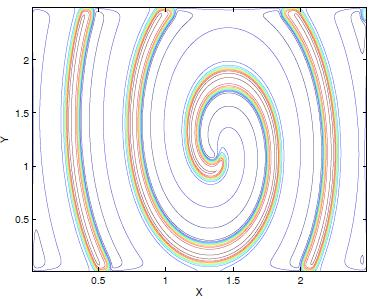
\includegraphics[width=4.5cm,height=4.5cm,scale=1]{figures/LiuKy=0.25Kx.jpg}
		\end{minipage}
	}
	\subfigure[]
	{
		\begin{minipage}{6cm}
			\centering
			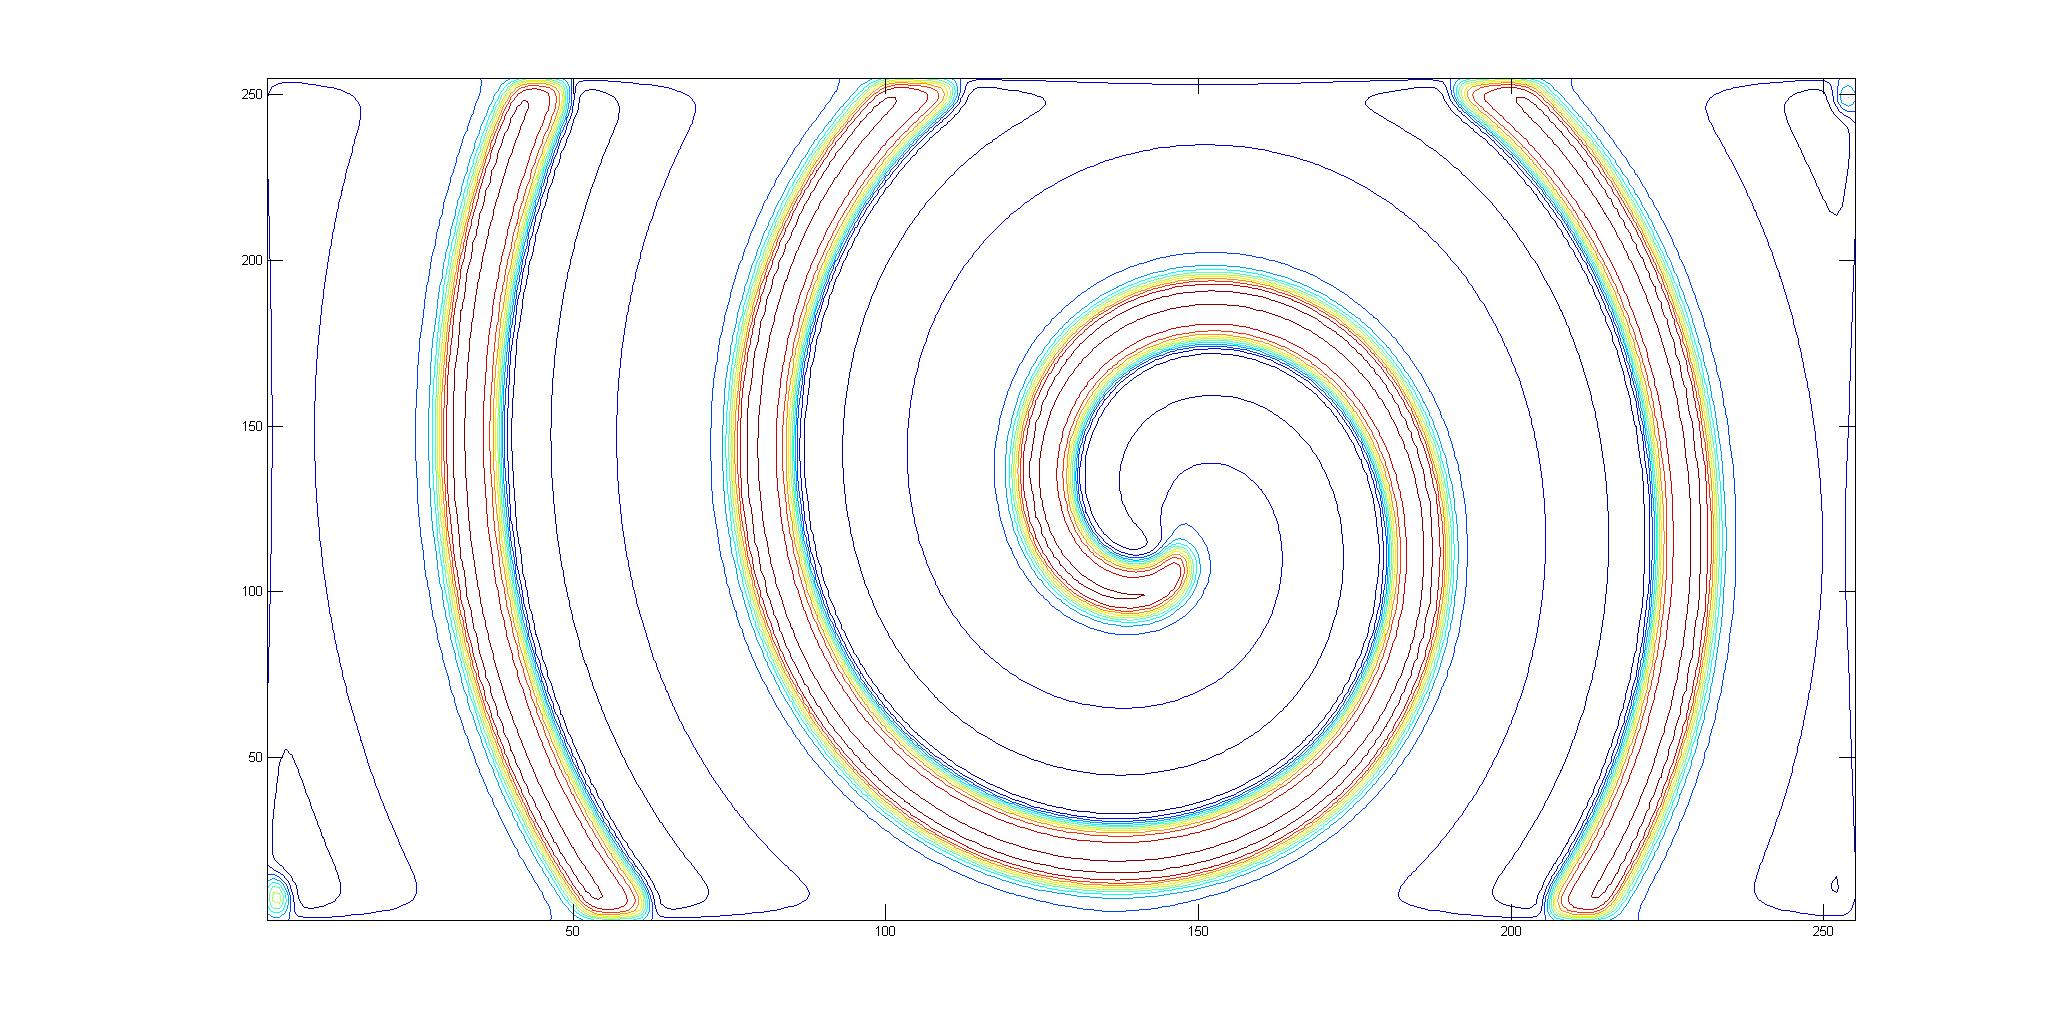
\includegraphics[width=5.1cm,height=5cm,scale=1]{figures/Ky=0.25Kx.jpg}
		\end{minipage}
	}
	\setlength{\abovecaptionskip}{-0.2cm} %调整图片标题与图距离 
	\caption{$K_{y}=10^{-4},K_{x}/K_{y} = 0.25$,跨膜电势$u$在$T=1000$时刻对比图}
	\label{fig:1b}
	\vspace{-0.5cm} %设定値自由调整
	
	\subfigure[]
	{
		\begin{minipage}{6cm}
			\centering
			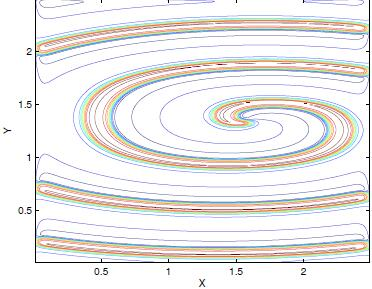
\includegraphics[width=4.5cm,height=4.5cm,scale=1]{figures/liuAlpha1=0.825Alpha2.jpg}
		\end{minipage}
	}
	\subfigure[]
	{
		\begin{minipage}{6cm}
			\centering
			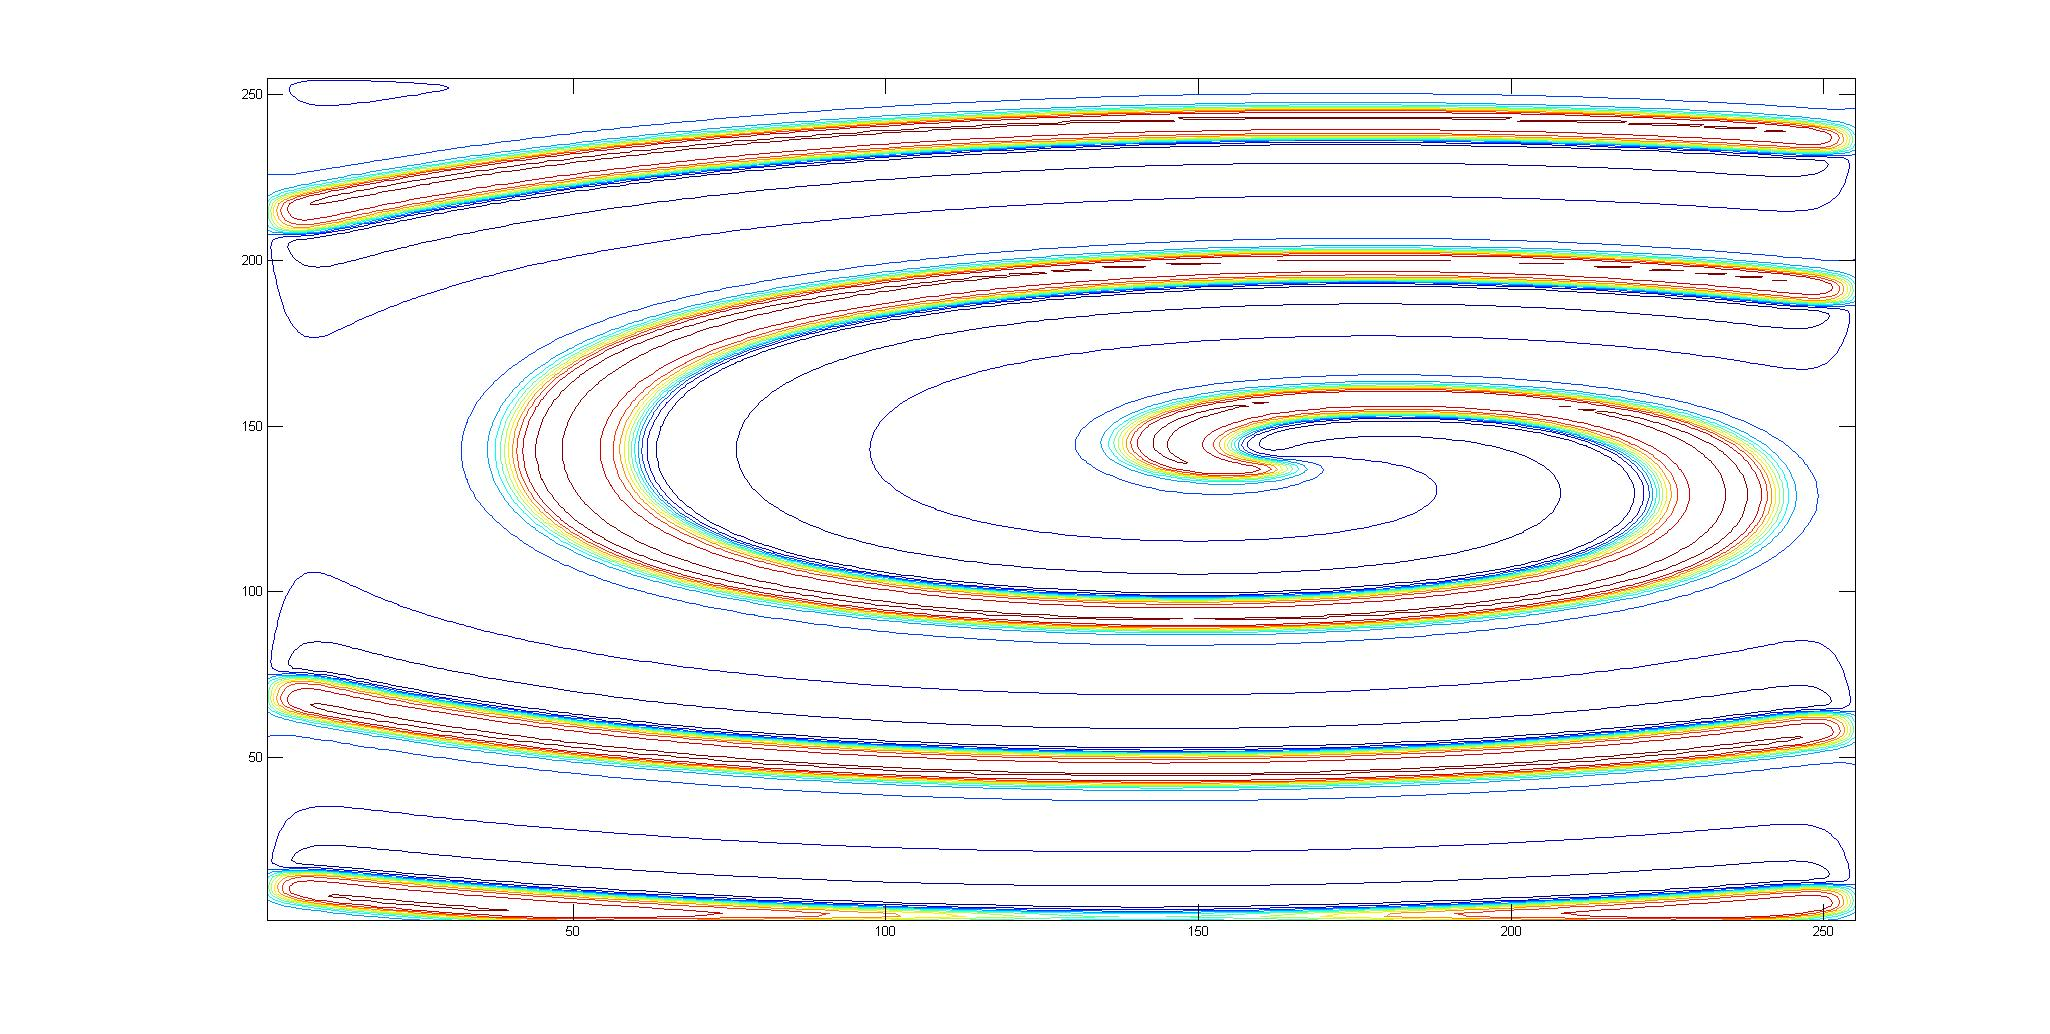
\includegraphics[width=5.1cm,height=5cm,scale=1]{figures/Alpha1=0.825Alpha2.jpg}
		\end{minipage}
	}
	\setlength{\abovecaptionskip}{-0.2cm} %调整图片标题与图距离 
	\caption{$\alpha_{1}=2,\alpha_{2}/\alpha_{1}=0.825$,跨膜电势$u$在$T=1000$时刻对比图}
	\label{fig:1a}
	\vspace{-0.5cm} %设定値自由调整	

	\subfigure[]
	{
		\begin{minipage}{6cm}
			\centering
			\includegraphics[width=4.5cm,height=4.5cm,scale=1]{figures/liuAlpha2=0.825Alpha1.jpg}
		\end{minipage}
	}
	\subfigure[]
	{
		\begin{minipage}{6cm}
			\centering
			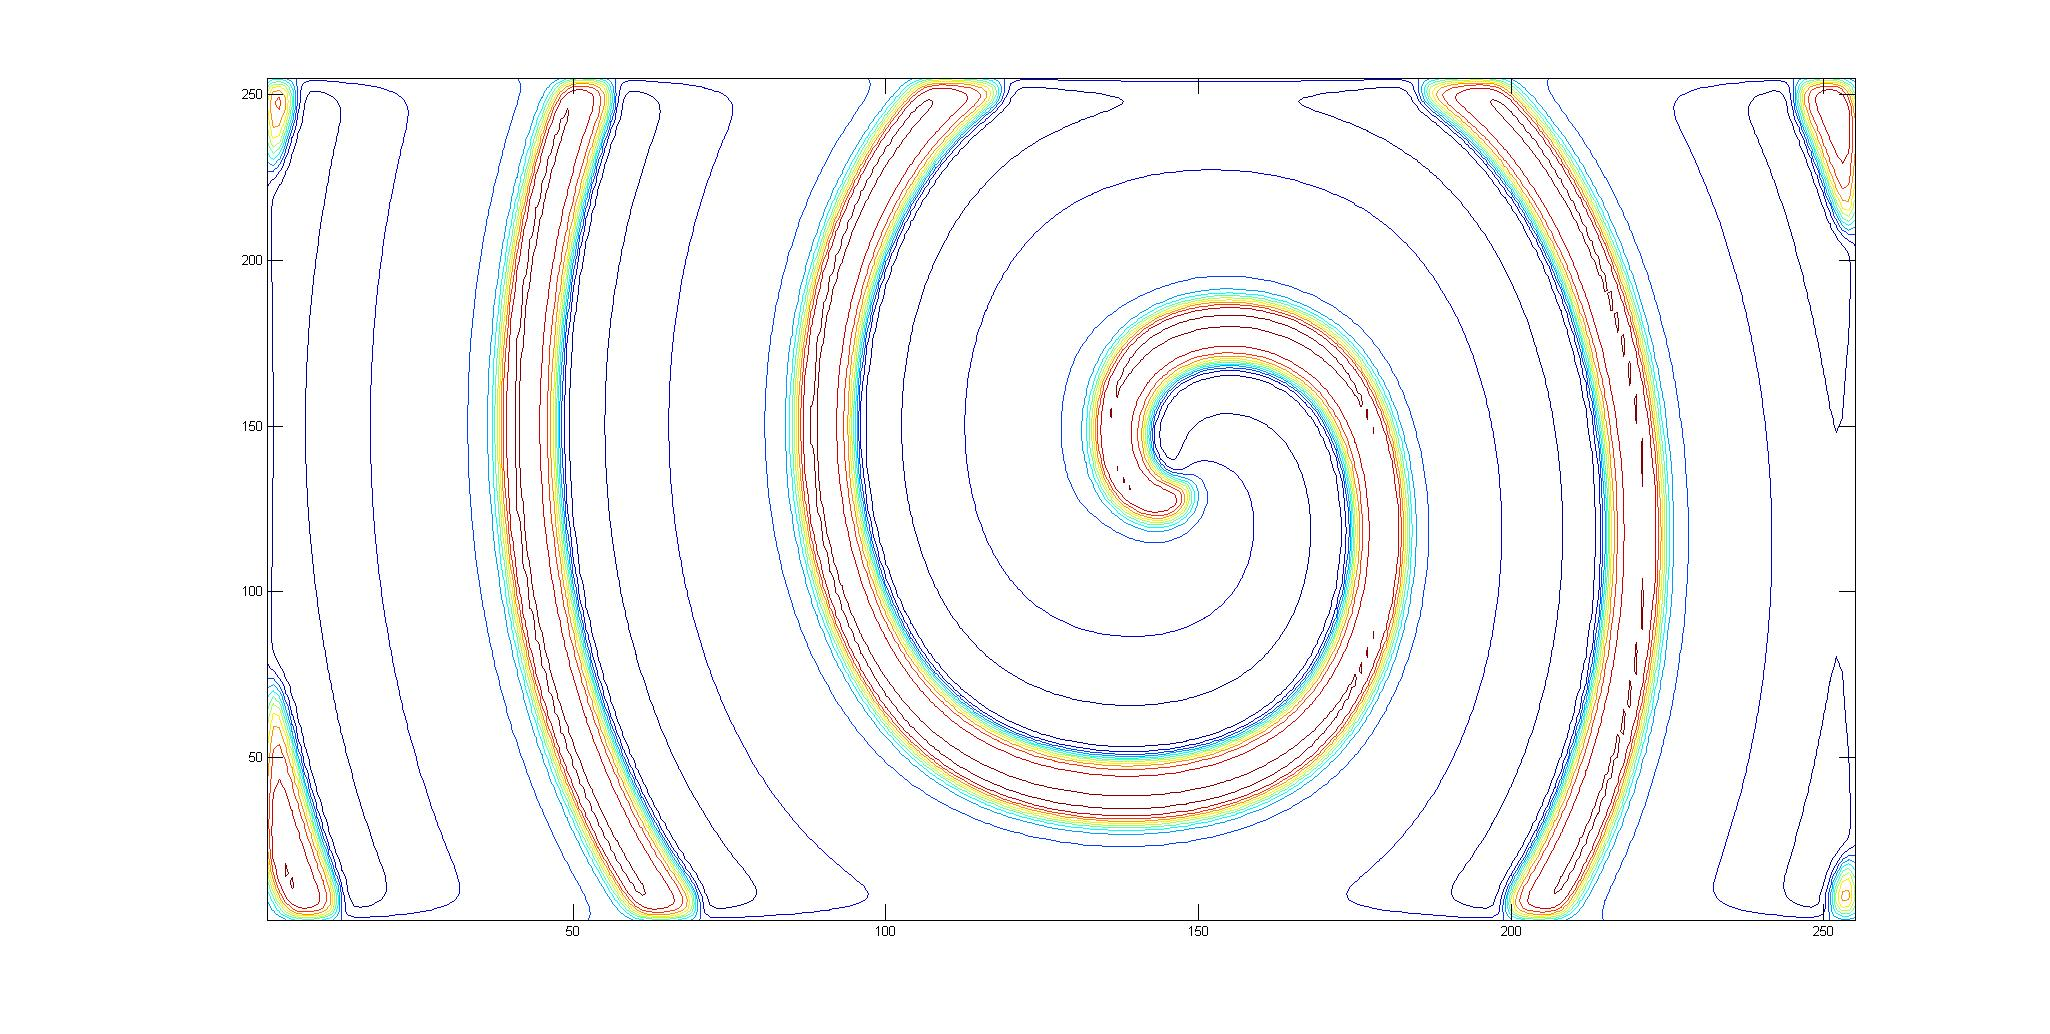
\includegraphics[width=5.1cm,height=5cm,scale=1]{figures/Alpha2=0.825Alpha1.jpg}
		\end{minipage}
	}
	\setlength{\abovecaptionskip}{-0.2cm} %调整图片标题与图距离 
	\caption{$\alpha_{2}=2,\alpha_{1}/\alpha_{2}=0.825$,跨膜电势$u$在$T=1000$时刻对比图}
	\label{fig:1b}
	\vspace{-0.5cm} %设定値自由调整
	
\end{figure}	
	
	

示图(4-7)-图(4-8)分别展示了具有各向异性的分数阶导数及扩散系数对于回火分数阶FHN模型计算结果的影响。当$x$方向上为整数阶,而$y$方向上为分数阶,与图(4-5)对比,跨膜电势$u$依然可以保持以螺旋波的形式自发而稳定地向外传播。螺旋波图像纵向压缩,呈现椭圆状的波形图案,这说明随着$y$方向上导数阶数的减小,激发波前的宽度减小,有限区域能够容纳的波数增加。类似的,与图(4-6)趋势一致,当减小$y$方向上的扩散系数,螺旋波呈现纵向压缩,这证明减小扩散系数与减小分数阶阶数对于计算结果具有一致的效果趋势,但是改变扩散系数与分数阶阶数对于计算结果影响的效果并不具有等价性,其他算例结果验证了上述规律。

\section{预处理共轭梯度法}
结合算例2给定的模型及初边值条件,分别采用共轭梯度法及针对Toeplitz矩阵及BTTB矩阵线性系统的预处理共轭梯度法进行计算。记录相同条件下使用三种不同的算法所消耗的CPU计算时间,验证预处理算法的实际计算效果。\\
\noindent   %当行不缩进
\textbf{例3}:针对于第三章所提出的预处理方案,设计相关算例验证不同方案的计算效果。\\
首先对Toeplitz线性系统(3-24)-(3-27)应用预处理共轭梯度法进行计算。设置分数阶${{\alpha }_{1}}={{\alpha}_{2}}=1.8$,扩散系数${{K}_{x}}={{K}_{y}}={{10}^{-4}}$,时间步长$\tau =0.1$,终止时间$T=100$,空间区域划分及相关参数的设定与例2相同。这里分别使用共轭梯度法(CG),针对于Toeplitz矩阵的预处理共轭梯度法(PCG)求解线性系统(3-24)-(3-27),并应用针对BTTB矩阵预处理共轭梯度法求解线性系统(3-29)。设置计算单步计算终止精度$tol=1\times {{10}^{-8}}$,最大迭代步数$\text{I}tem=100$。空间格点数分别设置为64,128,256,1024。对比三种计算方案所消耗的CPU时间。计算结果如表(4-3)所示。
\begin{table}[h]
	\centering

	%	\captiontitlefont{\xiaowuhao\bf }

	\caption[labelTabtab1]{共轭梯度法与预处理共轭梯度法计算CPU时间($s$)对比}
	\renewcommand\tabcolsep{1em}
	% \xiaowuhao \selectfont
	% \renewcommand{\arraystretch}{0.8}
	% \fontsize{9}{11}\selectfont
	\begin{tabular}{l|ccc}
		\toprule
		{N} &  {CG} & {Toeplitz-PCG } & {BTTB-PCG} \\
		\hline\hline
		64 & 0.012e+4 & 0.031e+3 & 0.087e+3\\
		128 & 0.034e+4 & 0.082e+3 & 0.232e+3\\
		256 & 0.094e+4	 & 0.210e+3 & 0.723e+3\\
		1024 & 3.779e+4 & 2.451e+3 & 7.521e+3\\
		
		\bottomrule
		\bottomrule
	\end{tabular}
\end{table}


表(4-3)记录了在相同的条件下应用三种算法计算回火FHN模型所消耗的CPU计算时间。相较于标准共轭梯度法,两种预处理共轭梯度法都大幅度的提高计算效率。通过对于计算量的理论分析可得针对于Toeplitz矩阵构造的PCG速度更快,实际计算过程中尽管涉及变量空间的开辟与赋值,迭代过程存储空间的使用对于计算时间有都有影响,但通过实际计算结果表明应用针对Toeplitz线性系统的预处理共轭梯度法的计算速度远远高于其他两种算法,尽管针对BTTB矩阵的线性系统的预处理算法计算速度略低,但依然远高于应用标准共轭梯度法的实际计算速度。这也间接证明了针对于BTTB矩阵提出的预处理方案的实际意义,该算法是一个高效的计算方案。通常地,针对多维分数阶扩散方程的有限差分格式构造过程中可以通过引入交错项分离为空间各个方向上独立的作用算子(参照Euler格式中ADI格式的构造过程)。本文将有限差分格式划分为多个子方程,而子方程矩阵形式为特殊的Toeplitz矩阵系统,这为应用预处理算法提供了必要的前提。本文应用方案1构造的Toeplitz预处理方法进行计算。另一方面,多维方程的有限差分格式可以直接转为矩阵形式,但是通常情况下矩阵构造复杂,矩阵的阶数也过于庞大,不利于直接进行计算。例如本文将二维有限差分格式直接转化为矩阵形式,方程的矩阵是特殊的BTTB矩阵,目前还没有针对BTTB矩阵系统的高效预处理方法出现,故对其的计算效率较低。本文使用方案2预处理方法进行计算,通过计算结果可以看出该方案相较于传统计算方法确实大幅度提高效率,为高效预处理方案。实际的计算效果往往与矩阵的阶数、参数的设定及计算方法的选择有关,因此合适的预处理方案需要结合数值实验进行选择。\\

\section{回火分数阶导数}
本节通过设计相关数值算例定量分析回火指数的改变对于数值计算结果的影响。\\
\noindent   %当行不缩进
\textbf{例4}:为了研究回火指数对于计算结果的影响效果,本例设置$\lambda =0.1$、$0.2$、$0.3$、$0.4$、$0.5$及$1$。空间分数阶阶数设置为$\alpha_{1}=\alpha_{2}=2.0$,扩散系数为${{K}_{x}}={{K}_{y}}={{10}^{-4}}$,其他参数设置同例2。计算在不同回火指数条件下相同时刻活跃电势$u$的传播规律。计算结果如图(4-13)所示。


\begin{figure}[h]
	\centering
	
	\subfigure[$\lambda=0.1$]
	{
	
		\begin{minipage}{4cm}
			\centering
			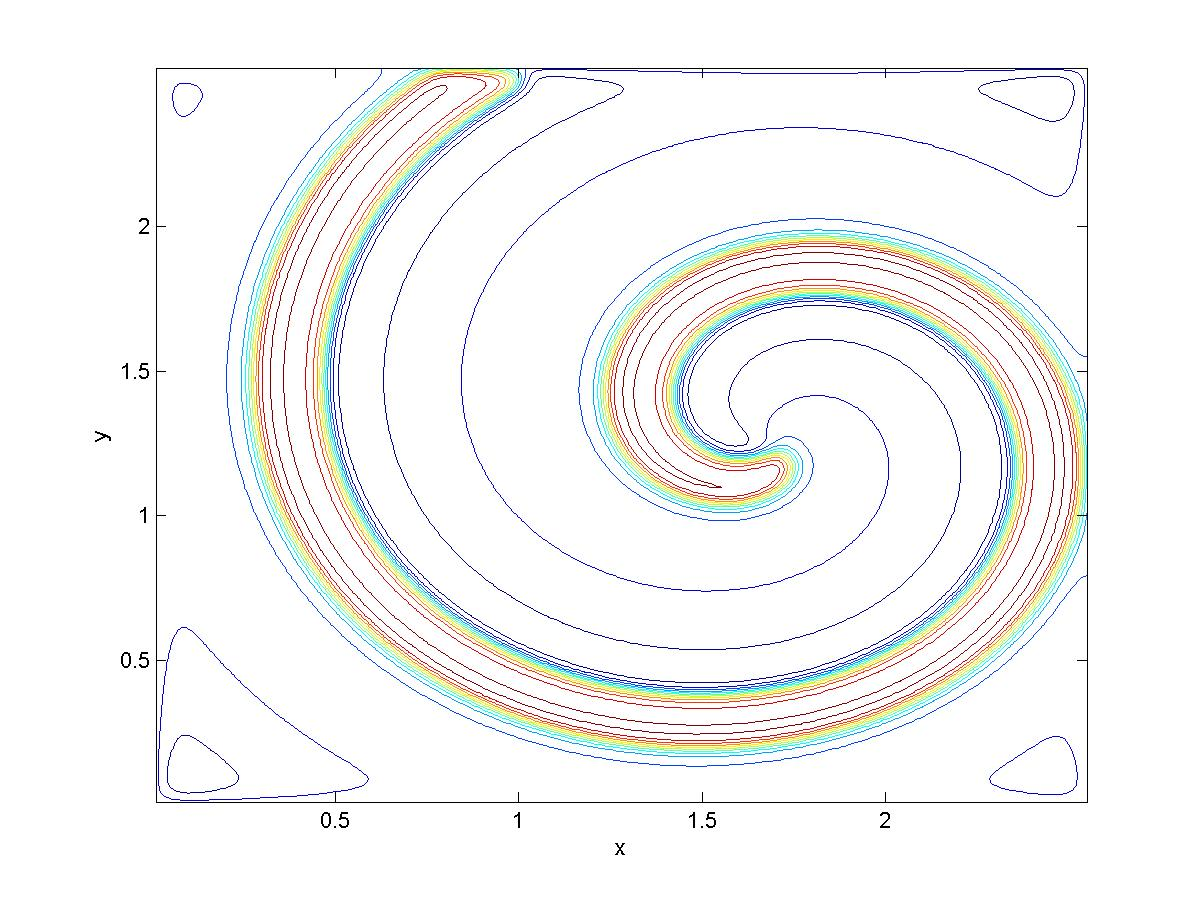
\includegraphics[width=4.5cm,height=4.5cm,scale=1]{figures/lamda=0.1.jpg}
		\end{minipage}
	}  
	\subfigure[$\lambda=0.2$]
	{
		\begin{minipage}{4cm}
			\centering
			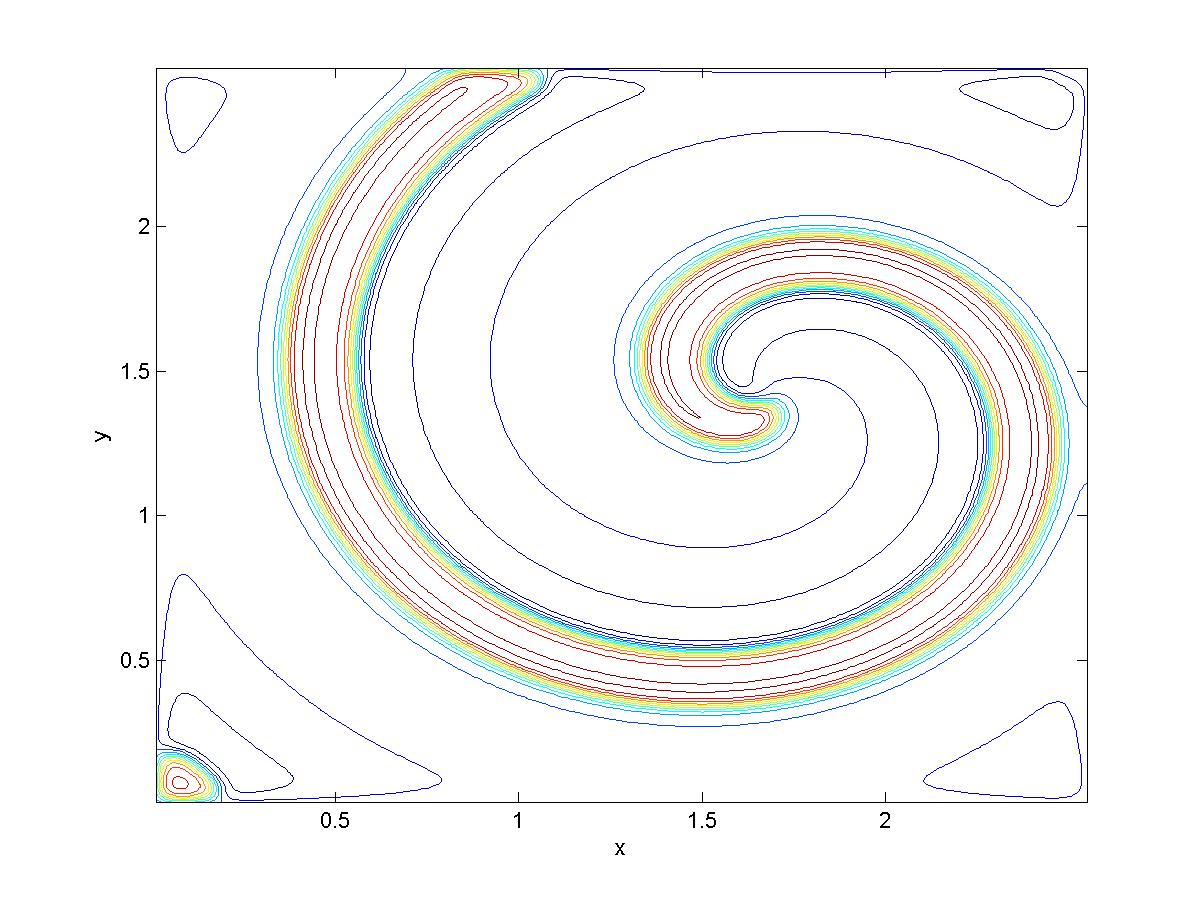
\includegraphics[width=4.5cm,height=4.5cm,scale=1]{figures/lamda=0.2.jpg}
		\end{minipage}
	}
	\subfigure[$\lambda=0.3$]
	{
		\begin{minipage}{4cm}
			\centering
			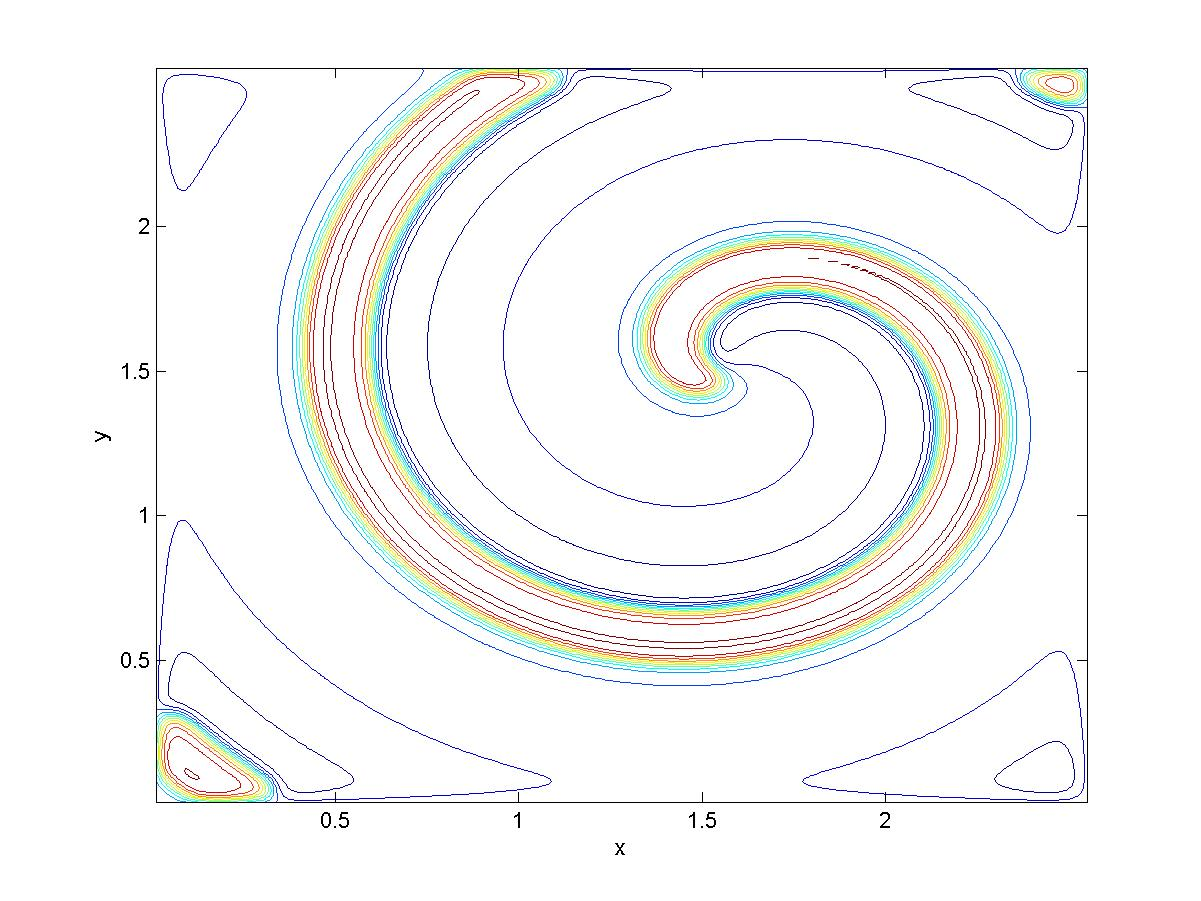
\includegraphics[width=4.5cm,height=4.5cm,scale=1]{figures/lamda=0.3.jpg}
		\end{minipage}
	}
		\subfigure[$\lambda=0.4$]
	{
		\begin{minipage}{4cm}
			\centering
			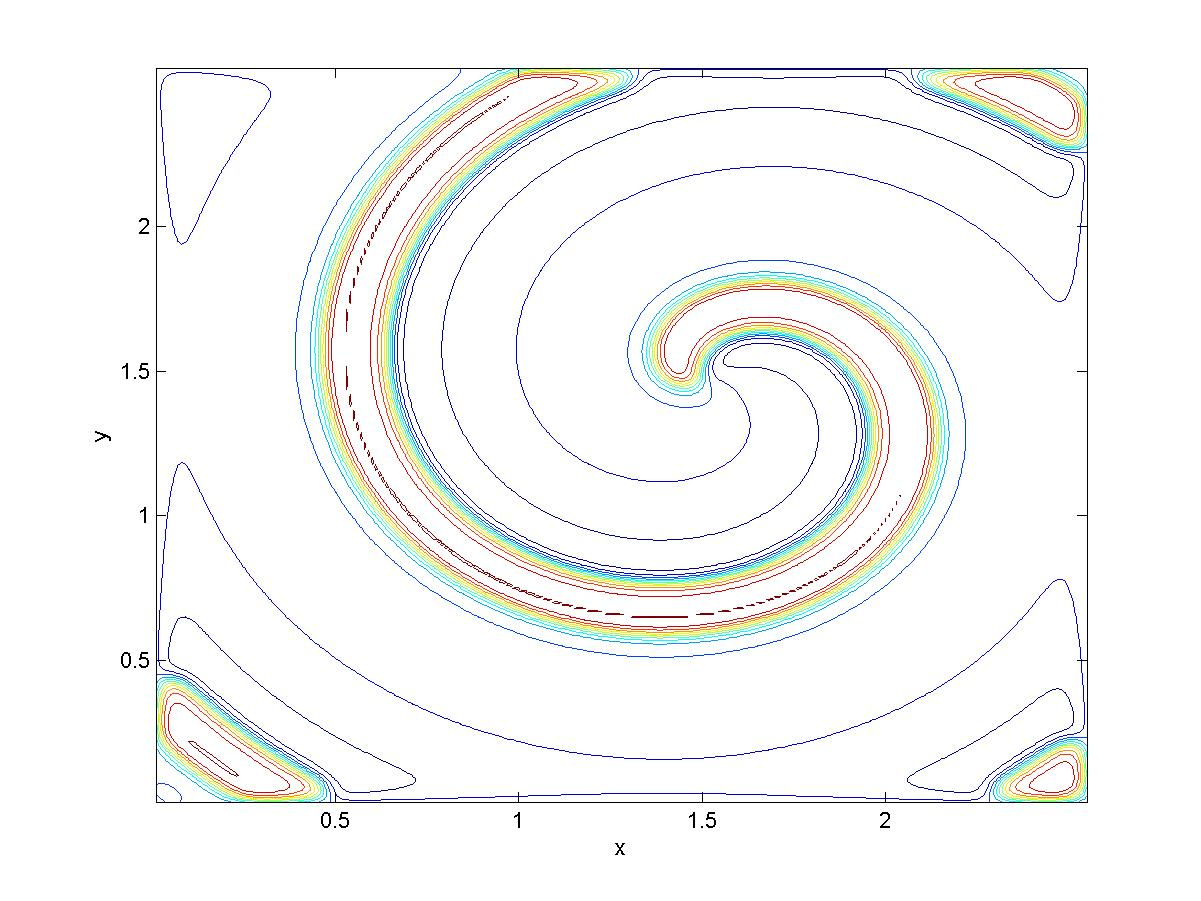
\includegraphics[width=4.5cm,height=4.5cm,scale=1]{figures/lamda=0.4.jpg}
		\end{minipage}
	}
	\subfigure[$\lambda=0.5$]
	{
		\begin{minipage}{4cm}
			\centering
			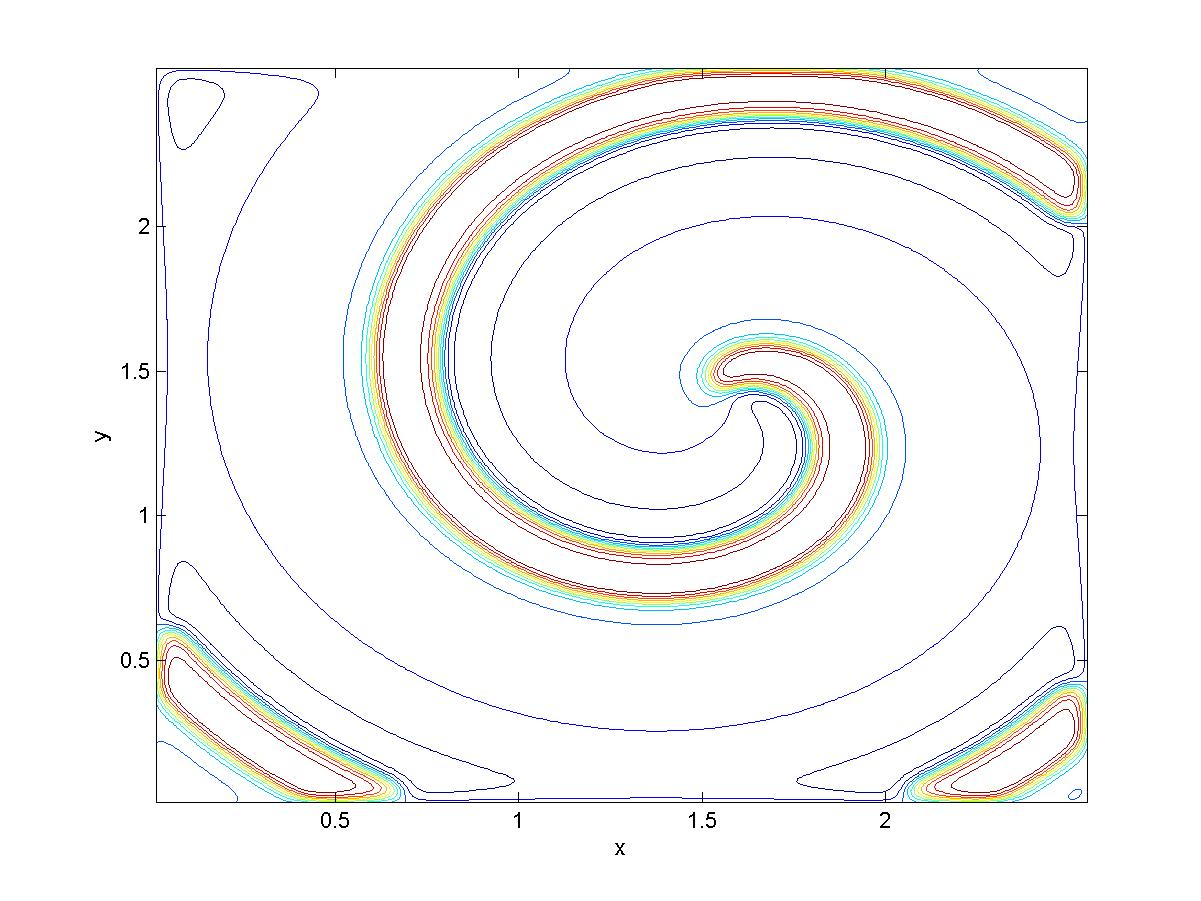
\includegraphics[width=4.5cm,height=4.5cm,scale=1]{figures/lamda=0.5.jpg}
		\end{minipage}
	}
	\subfigure[$\lambda=1$]
	{
		\begin{minipage}{4cm}
			\centering
			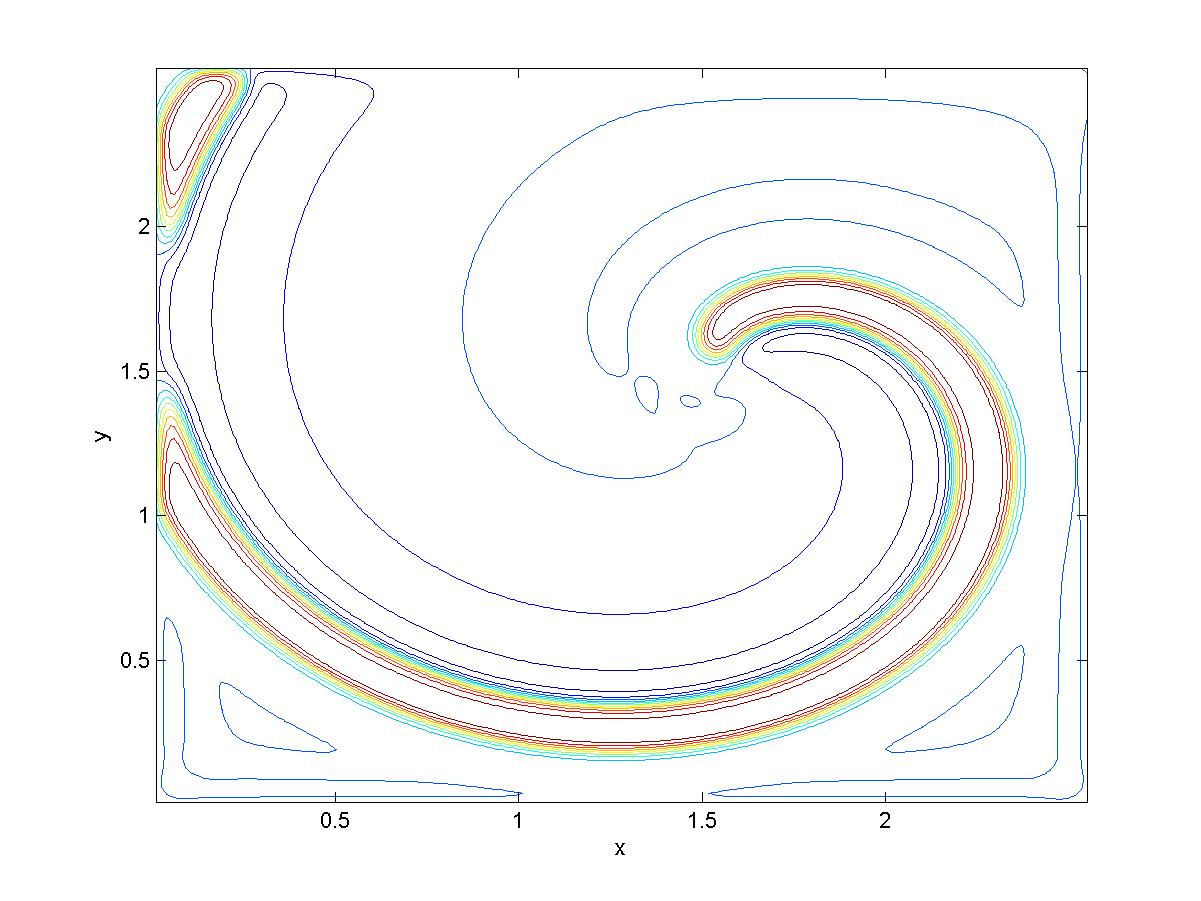
\includegraphics[width=4.5cm,height=4.5cm,scale=1]{figures/lamda=1.jpg}
		\end{minipage}
	}
	\setlength{\abovecaptionskip}{-0.2cm} %调整图片标题与图距离 
	\caption{$\alpha = 2.0,K_{x} = K_{y} = {10}^{-4}$,跨膜电势$u$在$T=1000$时刻对比图}
	\label{fig:1a}
	\vspace{-0.5cm} %设定値自由调整 

\end{figure}

从图(4-13)的计算结果可以看出,当只改变回火指数不会对于原有电势的传播形式造成影响,活跃电势$u$仍然以螺旋波的形式自发而稳定地向外扩散,激发波前的宽度未发生改变,与分数阶FHN模型在相同条件下的计算结果一致。另一方面,随着回火指数的增大,相同时刻的电势波形分布存在“滞后”现象,通过对于全局结果的对比印证了回火指数对于电势的传播速度造成影响。电势的传播速度随着回火指数$\lambda$的增大而减小。

为了定量计算回火指数的改变对于计算结果的影响,其他条件设置同上,分别取回火指数$\lambda =0$、$3$、$5$,观察空间区域中某个固定的节点$({{x}_{200}},{{y}_{100}})$上系统跨膜电势$u$随时间的变化情况,计算结果如图(4-14)所示。
\begin{figure}[h]
	\centering
	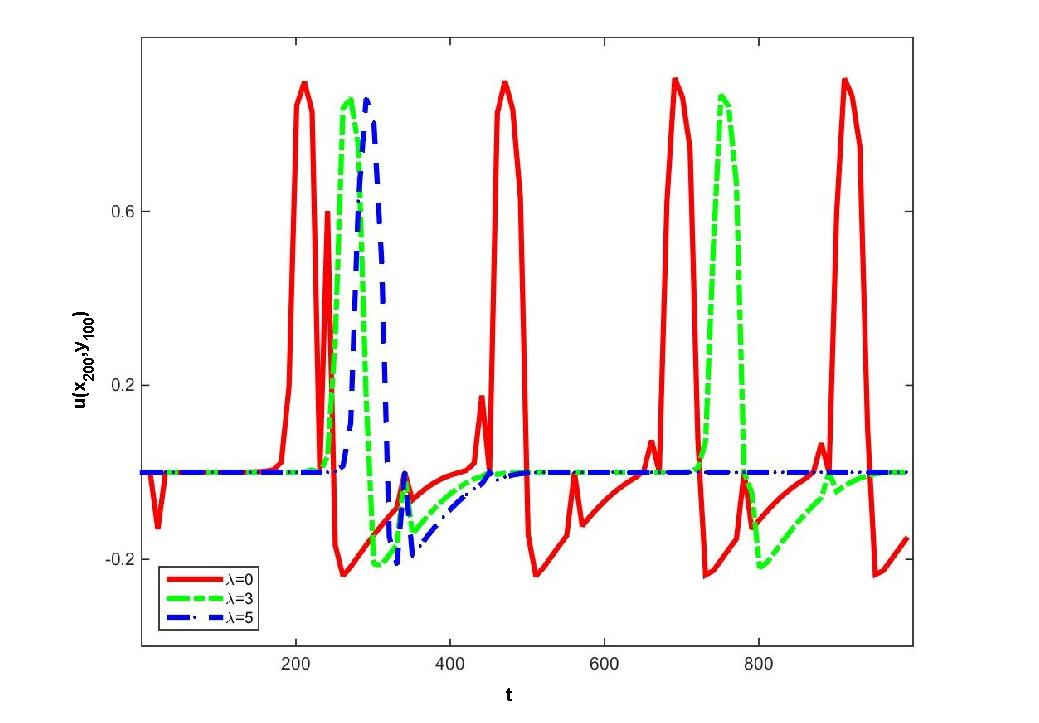
\includegraphics[width=0.8\textwidth,height=0.4\textwidth]{figures/Dotwave.jpg}
	\hspace{0.04\textwidth}
	\setlength{\abovecaptionskip}{-0.1cm} %调整图片标题与图距离 
	\caption{不同回火系数条件下节点$({{x}_{200}},{{y}_{100}})$电势$u$随时间变化情况}
\end{figure}

如图(4-14)所示,三条曲线变化分别代表不同回火指数条件下节点$({{x}_{200,}}{{y}_{100}})$上跨膜电势$u$随时间的变化情况。可以看出,同一条震荡曲线呈现出一定的周期性,这与实际情况相吻合,螺旋波在经过初值条件的影响后,逐渐形成稳定的螺旋波,向外匀速扩散。区域内格点上跨膜电势值随时间的变化的周期性,可以作为定量衡量螺旋波的扩散速度的指标。从图像中可以看出,随着回火指数$\lambda $的增大,图像首次出现震荡的波峰明显向后延迟,同时峰值明显减少,同一条曲线相邻波峰间隔时间也有所增加。证明随着回火指数的增大,螺旋波的扩散速度明显减慢。更进一步,为了定量衡量扩散速度的改变。设置其他条件不变,计算$T=5000$时间步中,同一曲线出现相邻两个震荡波峰间隔时间的平均值的倒数作为该螺旋波的平均扩散速度。计算结果如表(4-4)所示。
\begin{table}[h]
	\centering

	%	\captiontitlefont{\xiaowuhao\bf }
	\setlength{\abovecaptionskip}{0.2cm} %调整图片标题与图距离 
	\caption[labelTabtab1]{不同回火指数条件下电势传播速度对比}
	\renewcommand\tabcolsep{1em}
	% \xiaowuhao \selectfont
	% \renewcommand{\arraystretch}{0.8}
	% \fontsize{9}{11}\selectfont
	\begin{tabular}{cccc}
		\toprule
		{回火因子$\lambda $} &  {0} & {3} & {5} \\
		\midrule
		平均扩散速度 & 4.1918e-3 &2.0995e-3&1.2743e-3\\
		\bottomrule
	\end{tabular}
\end{table}

表(4-4)的计算结果定量显示随着回火指数$\lambda $的增大,回火分数阶导数对于扩散项的影响增大,螺旋波的扩散速度减慢。通常情况下,粒子反常扩散的扩散速度比正常扩散速度快\upcite{sabzikar2015tempered}。通过计算结果可以看出,随着回火指数$\lambda $的增大,回火项对于分数阶的截断作用加强,对于分数阶导数所模拟的粒子反常扩散运动限制加强,逐渐呈现出正常扩散的性质,回火分数阶扩散方程有效的模拟了“暂态反常扩散”过程。

此外,通过模拟空间区域上某个方向上跨膜电势$u$在固定时刻的分布情况,可以得到单个行波脉冲向外传播的变化曲线。其他条件设置同上,改变回火因子$\lambda =1,3,5,7,9$,记录在$T=1000$时刻下某条直线上$({{x}_{1-256}},{{y}_{50}})$跨膜电势$u$的分布情况。计算结果如图(4-15)所示。
\begin{figure}[htb]
	\centering
	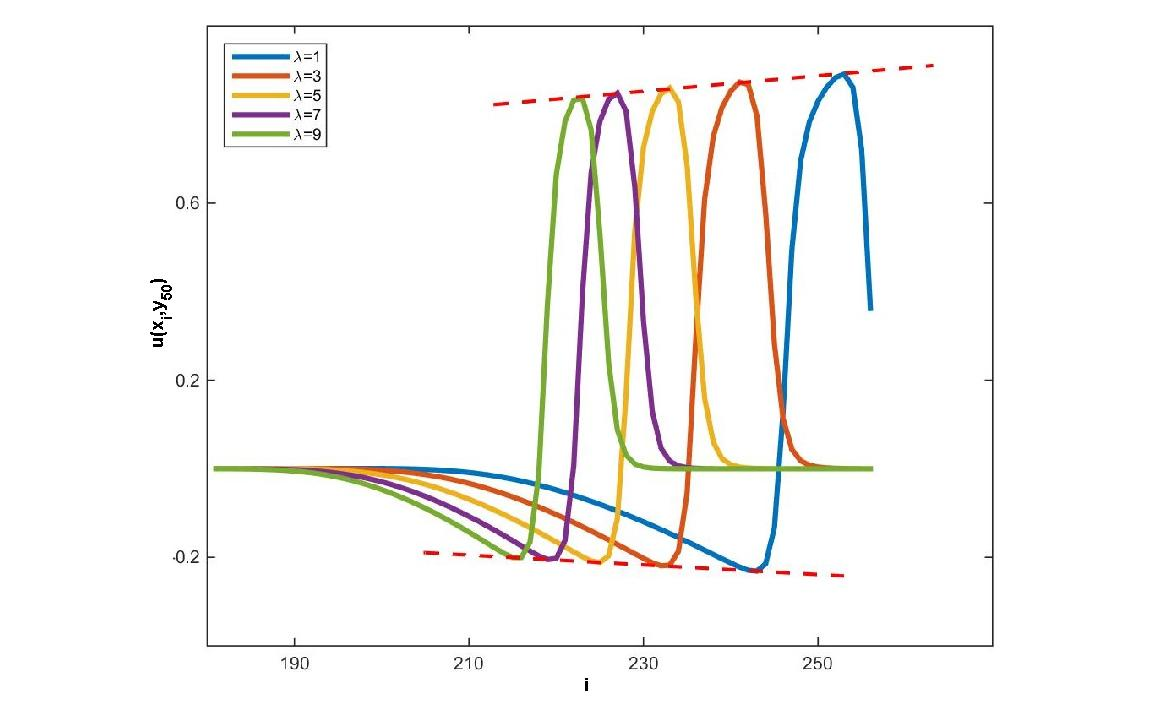
\includegraphics[width=0.8\textwidth,height=0.4\textwidth]{figures/hangwave.jpg}
	\hspace{0.04\textwidth}
	\setlength{\abovecaptionskip}{0.cm}
	\caption{相同时刻不同回火指数条件下直线上$({{x}_{1-256}},{{y}_{50}})$跨膜电势$u$的分布情况}
	\setlength{\belowcaptionskip}{-0.2cm}	
	\label{FCR} 
\end{figure}

通过图(4-15)可以看出,同一时刻下单一行波的波峰出现位置随着回火指数$\lambda $ 的减小向后分布,同时行波的振幅也逐渐加大,这与图(4-14)的计算结果一致,回火指数$\lambda $ 的增大减慢了螺旋波的扩散速度,并一定程度上增加了电势传播的峰值。综上所述,回火分数阶导数用来描述粒子受到扩散区域的及粒子生命周期的限制从反常扩散向正常扩散转变的过程,通过改变回火指数$\lambda $可以调节这种转变程度。\\
\noindent   %当行不缩进
\section{不规则区域上的电势传播}
本节分别在圆形区域、环形区域及心脏横向切片区域上计算回火分数阶FHN模型,验证第六章所构造的有限差分格式及算法在单连通不规则区域及多联通不规则区域上的实际计算效果。首先,构造算例在圆域上进行计算。\\
\noindent   %当行不缩进
\textbf{例5}:圆形区域的电势传播规律\\
定义圆形区域$\tilde{\Omega }=\{(x,y)|{{(r-x)}^{2}}+{{(r-y)}^{2}}\le {{r}^{2}},r=1.25\}$。其他参数设定与例2相同。为了方便验证计算结果的可靠性,置回火指数$\lambda =0$,即方程退化为标准分数阶FHN模型。\\
设置初值条件:
\[u(x, y, 0)=\left\{\begin{array}{cl}{1} & {r-\sqrt{r^{2}-(r-y)^{2}}<x \leq r \text { and }} \\ {} & {r-\sqrt{r^{2}-(r-x)^{2}}<y \leq r} \\ {0} & {\text { 其他 }}\end{array}\right.\]
\[v(x, y, 0)=\left\{\begin{array}{ll}{0.1} & {r-\sqrt{r^{2}-(r-y)^{2}}<x \leq r+\sqrt{r^{2}-(r-y)^{2}} \text { and }} \\ {} & {r<y \leq r+\sqrt{r^{2}-(r-x)^{2}}} \\ {0} & {\text { 其他 }}\end{array}\right.\]
边界条件为零Dirichlet条件。应用有限差分格式计算模型,扩散系数为${{K}_{x}}={{K}_{y}}={{10}^{-4}}$,${{K}_{x}}={{K}_{y}}={{10}^{-5}}$,分数阶阶数为${{\alpha }_{1}}={{\alpha }_{2}}=2.0$及${{\alpha }_{1}}={{\alpha }_{2}}=1.7$,在$T=1000$时刻数值结果如图(4-16)-(4-19)。

\begin{figure}[htbp]
	\centering
	
	\subfigure[]
	{
		\begin{minipage}{7cm}
			\centering
			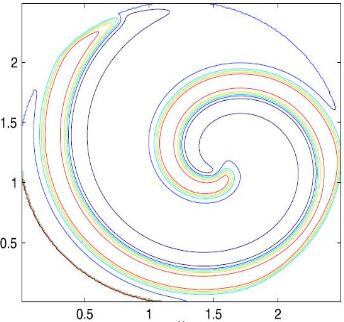
\includegraphics[width=5cm,height=5cm,scale=1]{figures/Circle_Alpha_2_Kx_1e-4ofLiu.jpg}
		\end{minipage}
	}
	\subfigure[]
	{
		\begin{minipage}{7cm}
			\centering
			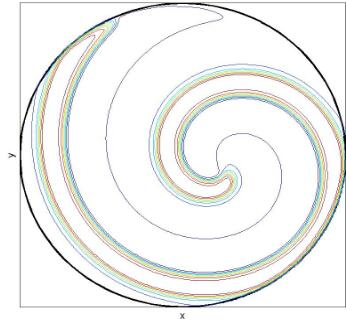
\includegraphics[width=5cm,height=5cm,scale=1]{figures/Circle_Alpha_2_Kx_1e-4.jpg}
		\end{minipage}
	}


	\setlength{\abovecaptionskip}{-0.2cm} %调整图片标题与图距离 
	\caption{$\alpha = 2.0,K_{x} = K_{y} = {10}^{-4}$,跨膜电势$u$在$T=1000$时刻对比图}
	\label{fig:1a}
	\vspace{-0.5cm} %设定値自由调整
	\subfigure[]
	{
		\begin{minipage}{7cm}
			\centering
			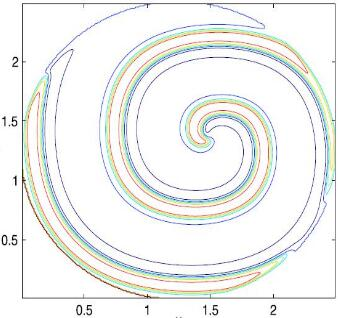
\includegraphics[width=5cm,height=5cm,scale=1]{figures/Circle_Alpha_1.8_Kx_1e-4ofLiu.jpg}
		\end{minipage}
	}
	\subfigure[]
	{
		\begin{minipage}{7cm}
			\centering
			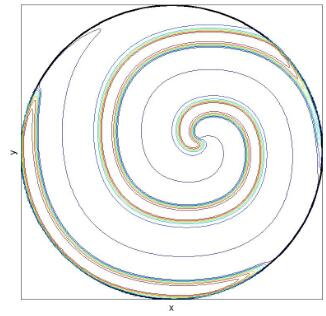
\includegraphics[width=5cm,height=5cm,scale=1]{figures/Circle_Alpha_1.8_Kx_1e-4.jpg}
		\end{minipage}
	}

	\caption{$\alpha = 1.8,K_{x} = K_{y} = {10}^{-4}$,跨膜电势$u$在$T=1000$时刻对比图}
	\label{fig:1b}
		\subfigure[]
	{
		\begin{minipage}{7cm}
			\centering
			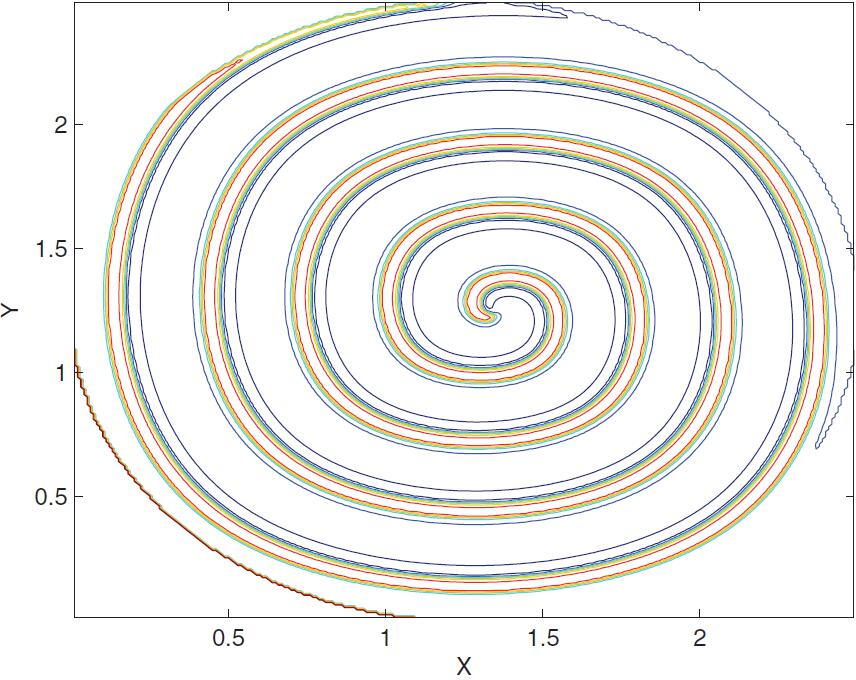
\includegraphics[width=5cm,height=5cm,scale=1]{figures/LiuCircleAlpha2_Kx_5.jpg}
		\end{minipage}
	}
	\subfigure[]
	{
		\begin{minipage}{7cm}
			\centering
			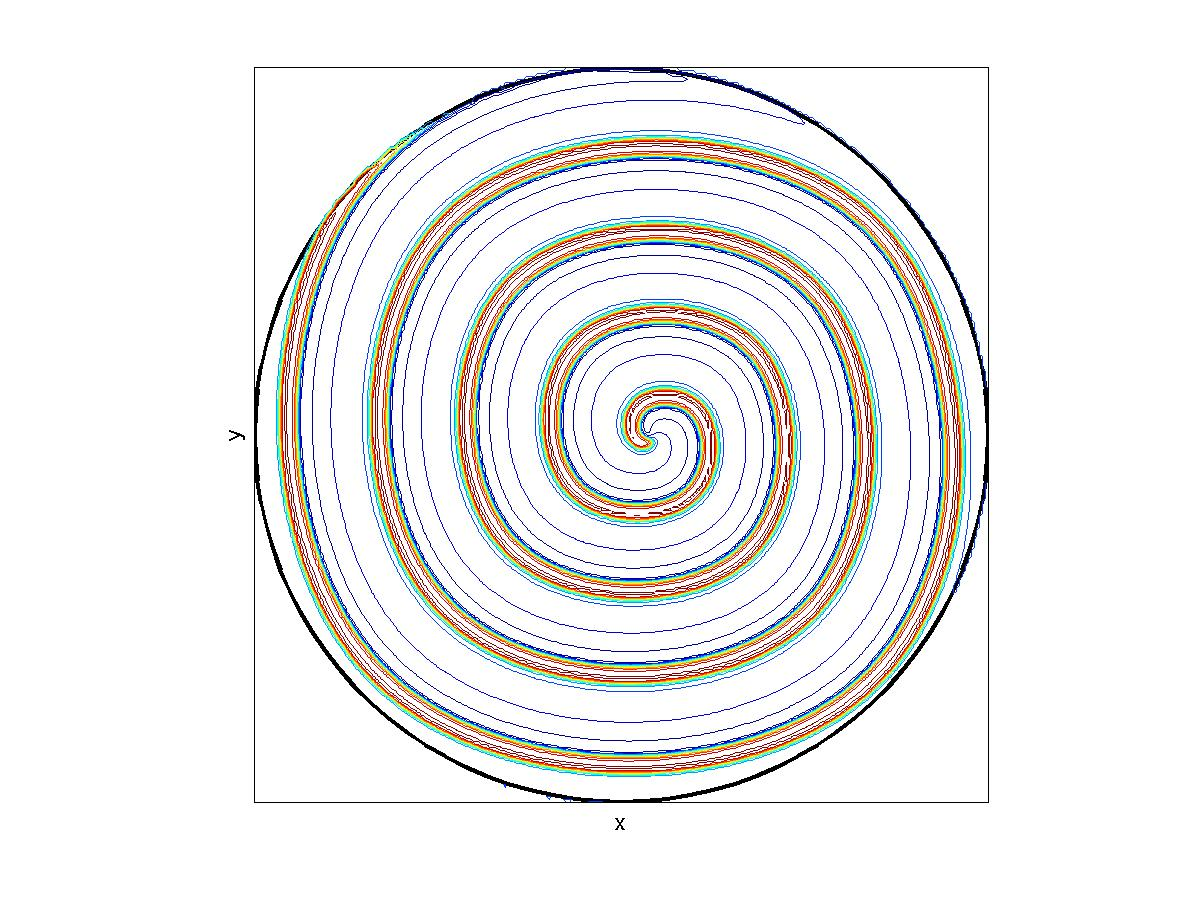
\includegraphics[width=7.5cm,height=5.5cm,scale=1]{figures/CircleAlpha2Kx1e-5.jpg}
		\end{minipage}
	}
	\setlength{\abovecaptionskip}{-0.2cm} %调整图片标题与图距离 
	\caption{$\alpha = 2.0,K_{x} = K_{y} = {10}^{-5}$,跨膜电势$u$在$T=1000$时刻对比图}
	\label{fig:1b}
	\vspace{-0.5cm} %设定値自由调整
	
	
	\subfigure[]
	{
		\begin{minipage}{7cm}
			\centering
			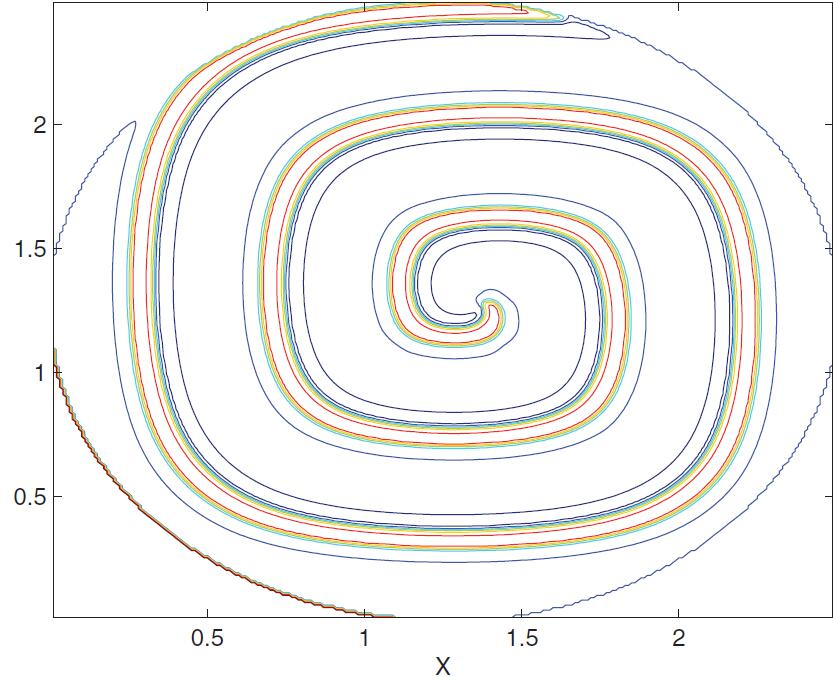
\includegraphics[width=5cm,height=5cm,scale=1]{figures/LiuCircleAlpha1.6.jpg}
		\end{minipage}
	}
	\subfigure[]
	{
		\begin{minipage}{7cm}
			\centering
			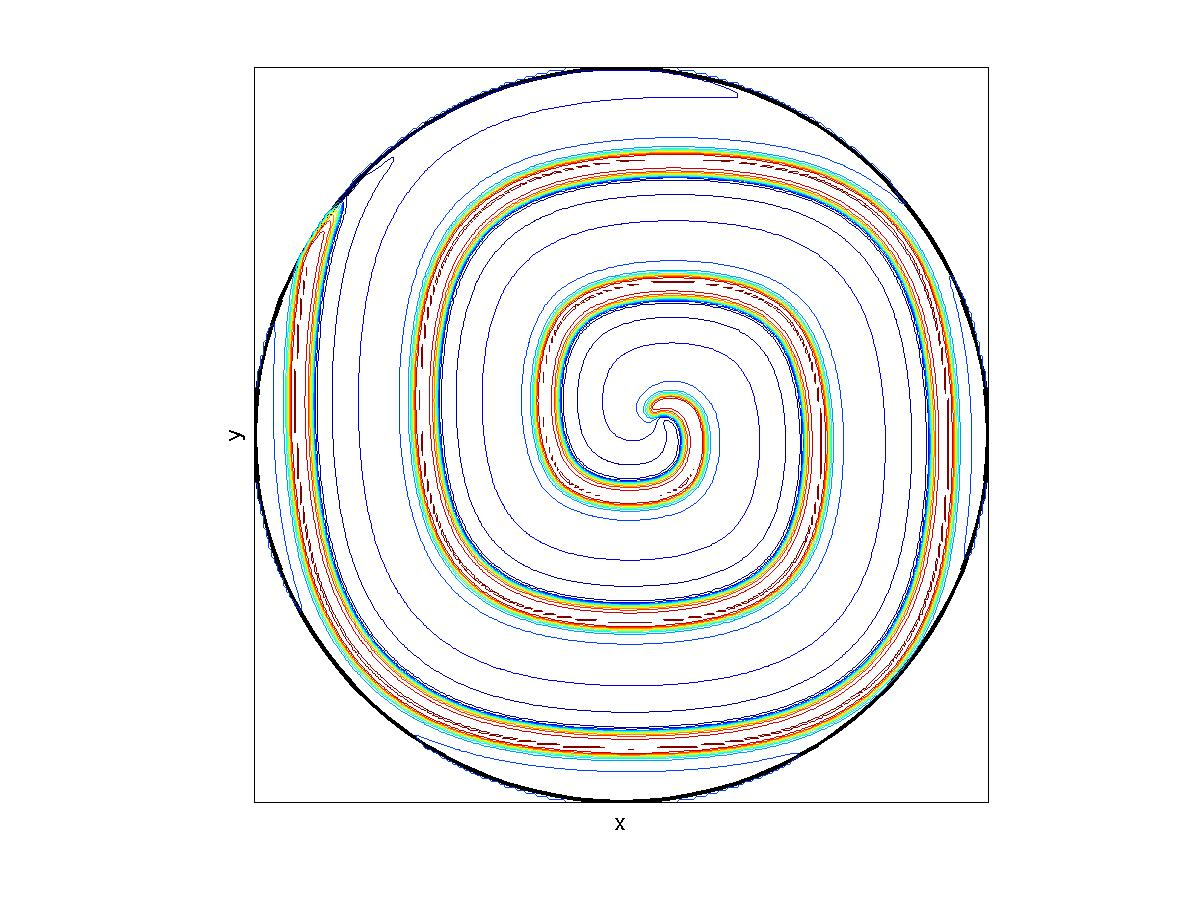
\includegraphics[width=7.5cm,height=5.5cm,scale=1]{figures/CircleAlpha1.6.jpg}
		\end{minipage}
	}
	\setlength{\abovecaptionskip}{-0.2cm} %调整图片标题与图距离 
	\caption{$\alpha = 1.6,K_{x} = K_{y} = {10}^{-4}$,跨膜电势$u$在$T=1000$时刻对比图}
	\label{fig:1b}
	\vspace{-0.5cm} %设定値自由调整
	

	
	
	
\end{figure}


从图(4-16)-(4-19)中显示的计算结果可得,当$\lambda =0$时,数值格式的计算结果(右图)与Liu 的计算结果(左图)\upcite{liu2015semi}基本一致,说明有限差分格式(3-22)-(3-23)适用于在凸单连通不规则区域上进行计算。同时可以看出,尽管跨膜电势$u$传播受到圆形边界区域的限制,波形图像依然能够基本保持螺旋波的形状,自发而稳定地向外扩散,这与方形区域上计算结果保持一致。此外,当空间分数阶阶数减小的时候激发波前的宽度随之减小,在有限区域上所能够容纳的波数随之增加,这与减小扩散系数产生的趋势基本一致,随着扩散系数的减小,有限空间上的螺旋波变得更加稠密。但是,改变分数阶阶数与改变扩散系数对于计算结果的影响并不完全一致,不具有可替换性。尽管受到空间区域的限制使得螺旋波的波形与相同条件下方形区域上所计算的结果不完全一致,但电势波传播形式及相关参数的改变对于数值结果造成的影响基本保持一致。\\

                                                                                   
\noindent   %当行不缩进
\textbf{例6}:环形区域的电势传播规律\\
定义环形区域$\tilde{\Omega }$:${{r}_{2}}^{2}\le {{({{r}_{1}}-x)}^{2}}+{{({{r}_{1}}-y)}^{2}}\le {{r}_{1}}^{2}$,其中${{r}_{1}}=1.25$,${{r}_{2}}=0.2$。应用有限差分格式(3-22)及算法1进行计算,其他相关参数设置同上 ,令回火指数$\lambda =0$,计算${{\alpha }_{1}} ={{\alpha }_{2}} =2\text{.0}$,${{K}_{x}}={{K}_{y}}={{10}^{-4}}$时的计算结果。
边值条件设为零Direchilet边值条件。初值条件设为\\
\[
u(x, y, 0)=\left\{\begin{array}{ccc}{1} & {0 \leq y \leq r_{1}-r_{2}, r_{1}-\sqrt{r_{1}^{2}-\left(r_{1}-y\right)^{2}}<x \leq r_{1}} \\ {} & {r_{1}-r_{2} \leq y \leq r_{1}, r_{1}-\sqrt{r_{1}^{2}-\left(r_{1}-y\right)^{2}}<x \leq r_{2}-\sqrt{r_{2}^{2}-\left(r_{2}-y\right)^{2}}} \\ {0} & { \text{其他} }\end{array}\right.
\]
\[
v(x, y, 0)=\left\{\begin{array}{ccc}{0.1} &{ r_{1}+r_{2}<y \leq 2 r_{1}, r_{1}-\sqrt{r_{1}^{2}-\left(r_{1}-y\right)^{2}}<x \leq r_{1}+\sqrt{r_{1}^{2}-\left(r_{1}-y\right)^{2}}} \\ &{r_{1}<y \leq r_{1}+r_{2}, r_{1}-\sqrt{r_{1}^{2}-\left(r_{2}-y\right)^{2}}<x<r_{2}-\sqrt{r_{2}^{2}-\left(r_{2}-y\right)^{2}}} \\ &{r_{1}<y \leq r_{1}+r_{2}, r_{2}+\sqrt{r_{2}^{2}-\left(r_{2}-y\right)^{2}}<x<r_{1}+\sqrt{r_{1}^{2}-\left(r_{1}-y\right)^{2}}} \\
{0}  &{\text{其他}}\end{array}\right.
\]
\begin{figure}[htbp]
	\centering
	\subfigure[t=250]
	{
		\begin{minipage}{7cm}
			\centering
			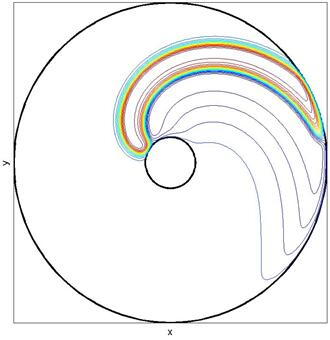
\includegraphics[width=5cm,height=5cm,scale=1]{figures/Loop1.jpg}
		\end{minipage}
	}
	\subfigure[t=300]
	{
		\begin{minipage}{7cm}
			\centering
			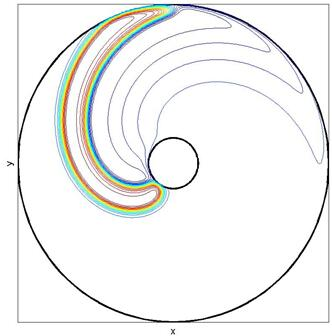
\includegraphics[width=5cm,height=5cm,scale=1]{figures/Loop2.jpg}
		\end{minipage}
	}
	
	\subfigure[t=450]
	{
		\begin{minipage}{7cm}
			\centering
			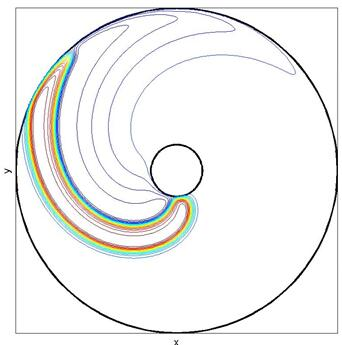
\includegraphics[width=5cm,height=5cm,scale=1]{figures/Loop3.jpg}
		\end{minipage}
		
	}
	\subfigure[t=550]
	{
		\begin{minipage}{7cm}
			\centering
			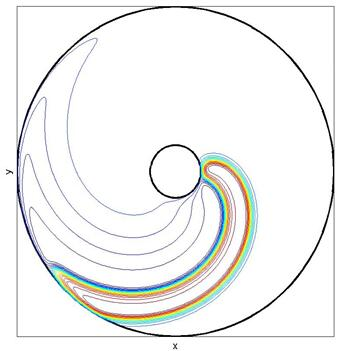
\includegraphics[width=5cm,height=5cm,scale=1]{figures/Loop4.jpg}
		\end{minipage}
		
	}
	\setlength{\abovecaptionskip}{-0.2cm} %调整图片标题与图距离 
	\caption{环域电势传播规律}
	\label{fig:1a}	
	\vspace{-0.5cm} %设定値自由调整

\end{figure}

\renewcommand{\figurename}{图}
计算结果如图(4-20)所示,通过在环形区域上对于回火分数阶FHN模型的计算结果可以看出,有限差分格式(3-22)-(3-23)与算法1符合实际计算的要求。此外,由于空间区域对于电势传播过程限制的加强,环形区域上的电势传播将不再以螺旋波的形式进行传播。电势传播的波头围绕内圆圆周逆时针旋转传播,呈现出自发稳定周期性的传播形式,相较于单联通区域上电势传播形式存在差异。同样地,激发波前的宽度受到方程空间分数阶阶数及扩散系数的控制,而电势传播的速度受到回火指数的控制,与单连通区域上模型的计算结果保持一致。\\
\noindent   %当行不缩进
\textbf{例7}:心脏横向切片区域的电势传播规律\\
为了验证算法1的鲁棒性。本文应用有限差分格在真实的人类心脏横向切片计算回火分数阶FHN模型,设置网格格点为$256\times 256$,相关参数及初边值条件的设定同例2,分数阶为${{\alpha }_{1}}={{\alpha }_{2}}=2.0$,计算在T=2000时刻内电势传播规律。

\begin{figure}[htbp]
	\centering
	
	\subfigure[$T=1000$]
	{
		
		\begin{minipage}{4cm}
			\centering
			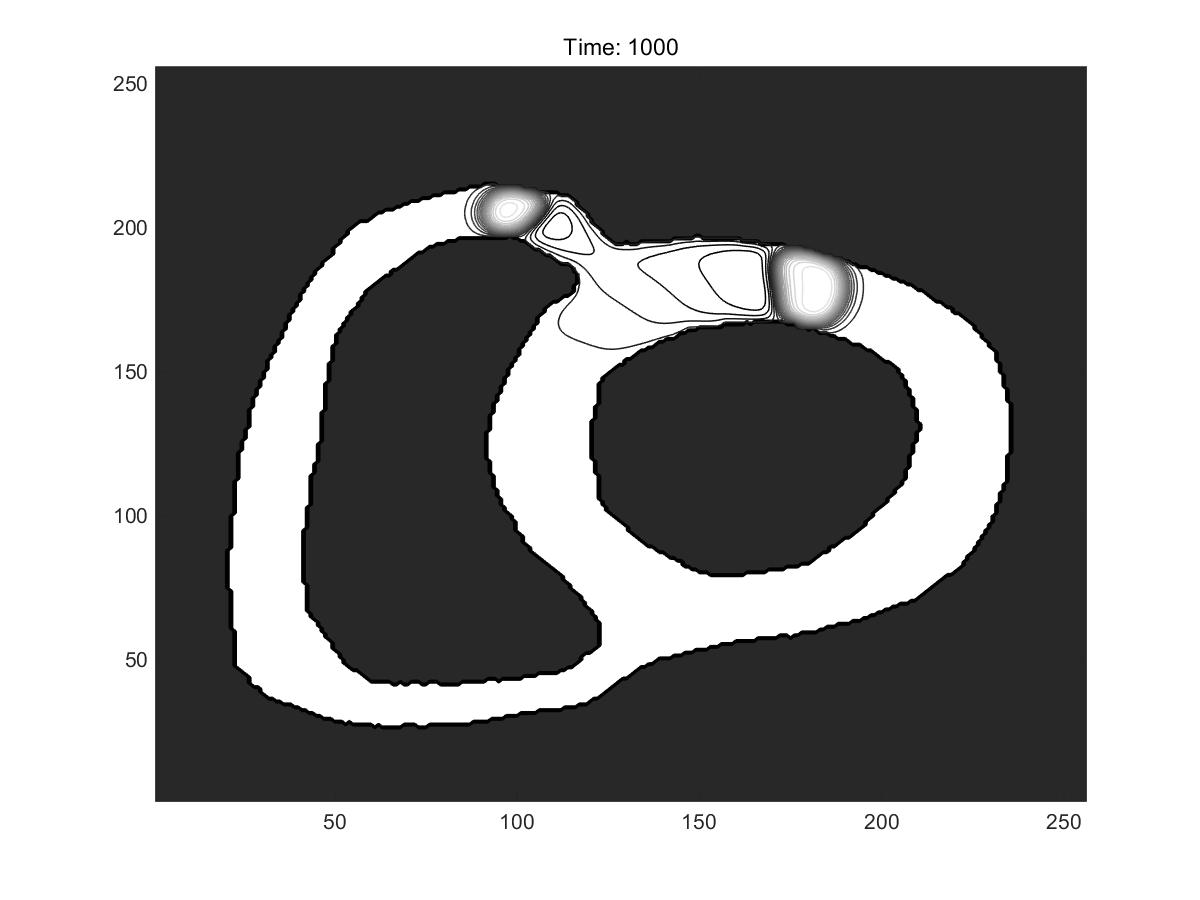
\includegraphics[width=4.5cm,height=4.5cm,scale=1]{figures/Lay100.jpg}
		\end{minipage}
	}  
	\subfigure[$T=1380$]
	{
		\begin{minipage}{4cm}
			\centering
			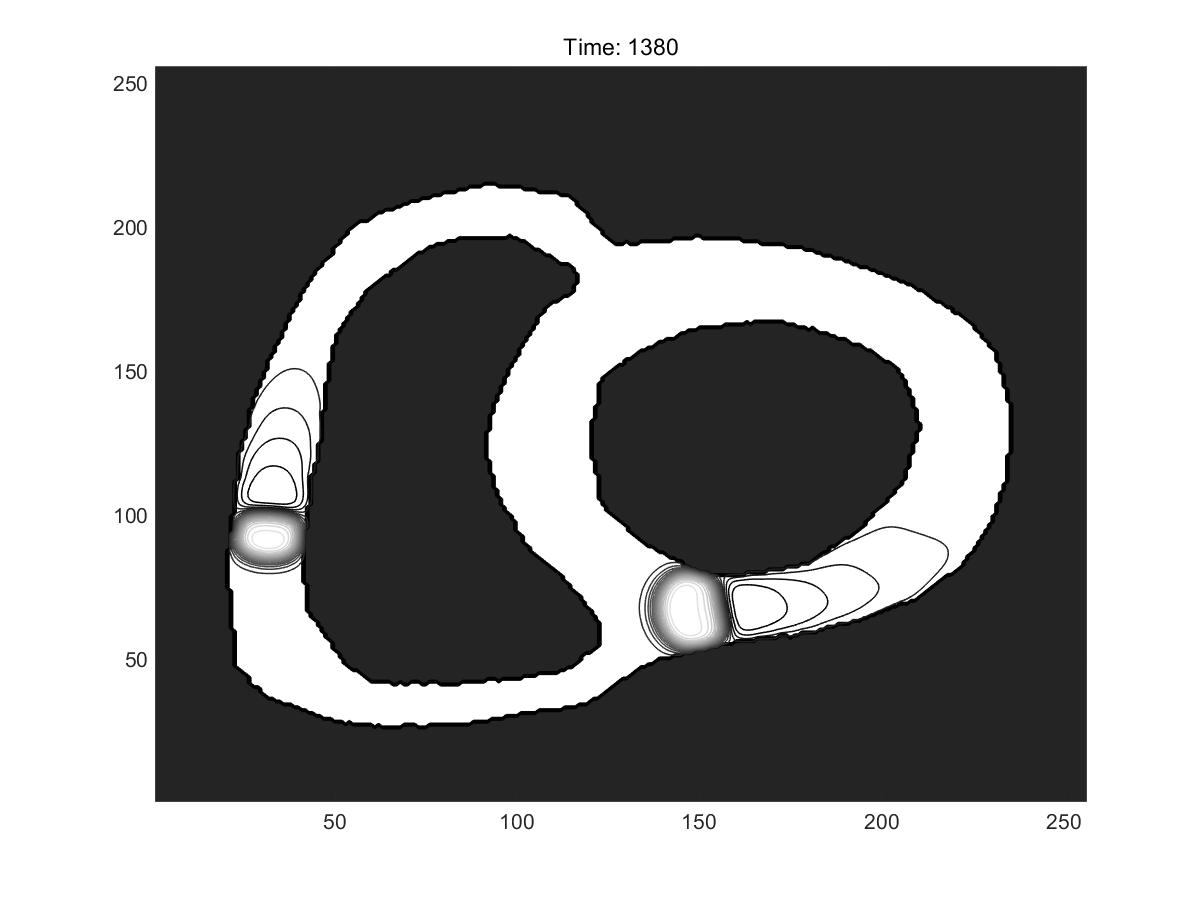
\includegraphics[width=4.5cm,height=4.5cm,scale=1]{figures/Lay138.jpg}
		\end{minipage}
	}
	\subfigure[$T=1450$]
	{
		\begin{minipage}{4cm}
			\centering
			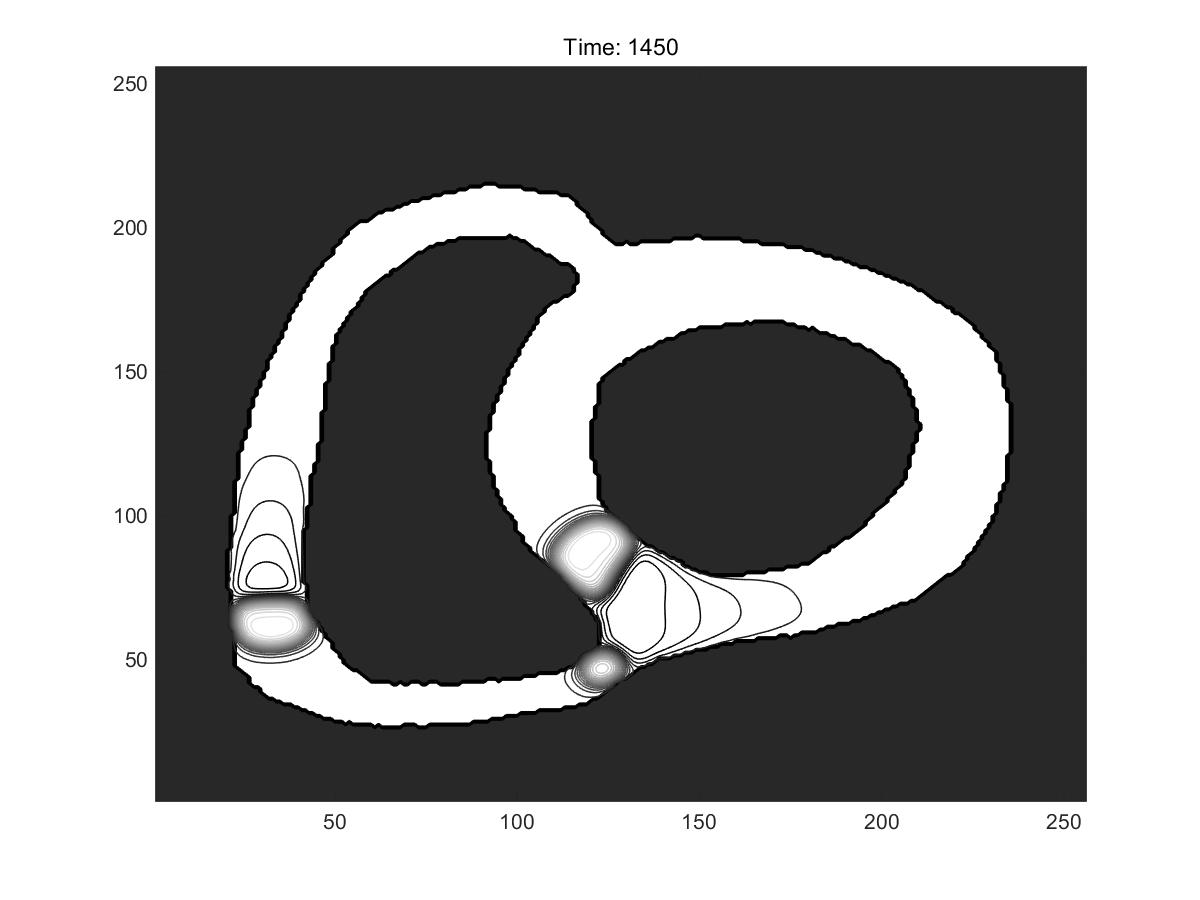
\includegraphics[width=4.5cm,height=4.5cm,scale=1]{figures/Lay145.jpg}
		\end{minipage}
	}
	\subfigure[$T=1580$]
	{
		\begin{minipage}{4cm}
			\centering
			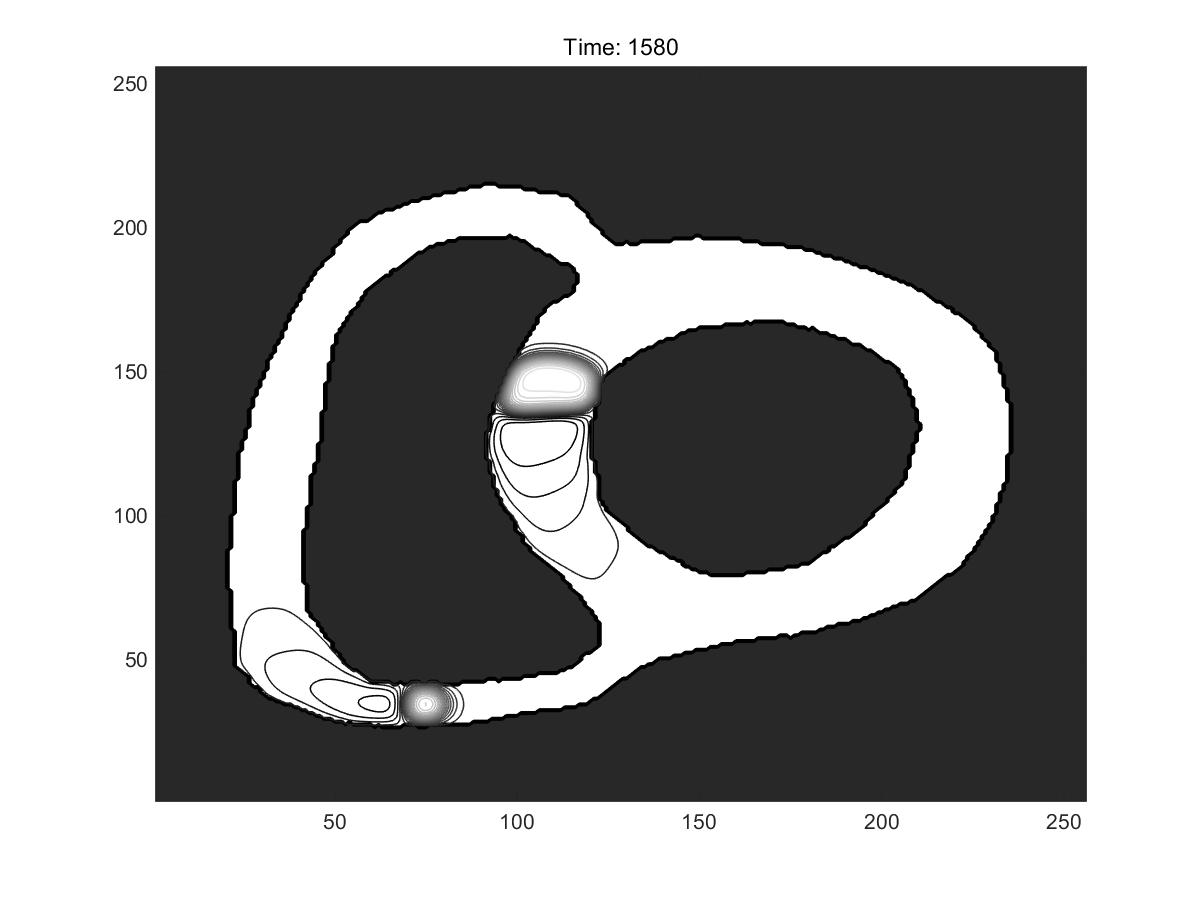
\includegraphics[width=4.5cm,height=4.5cm,scale=1]{figures/Lay158.jpg}
		\end{minipage}
	}
	\subfigure[$T=1810$]
	{
		\begin{minipage}{4cm}
			\centering
			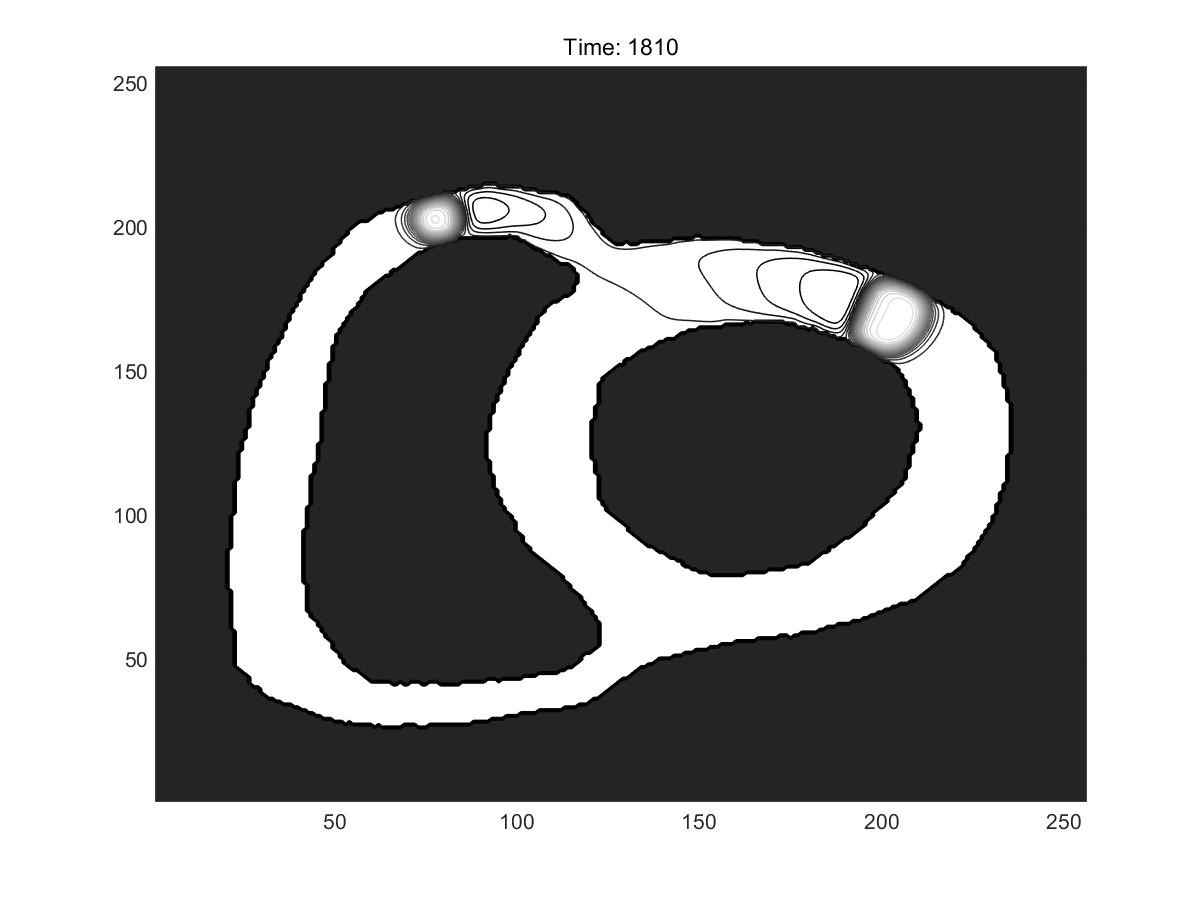
\includegraphics[width=4.5cm,height=4.5cm,scale=1]{figures/Lay181.jpg}
		\end{minipage}
	}
	\subfigure[$T=1950$]
	{
		\begin{minipage}{4cm}
			\centering
			\includegraphics[width=4.5cm,height=4.5cm,scale=1]{figures/Lay195.jpg}
		\end{minipage}
	}

	\setlength{\abovecaptionskip}{-0.2cm} %调整图片标题与图距离 
	\caption{心脏横向切片电势传播}
	\label{fig:1a}
	\vspace{-0.5cm} %设定値自由调整 
	
\end{figure}


通过对于计算结果进行分析可得,与上面算例的计算结果相比较,复杂的多联通区域对于电势传播的限制继续加强,电势传播不再呈现以螺旋波的形式自发而稳定地传播,与例6计算结果类似于“团状”的波形围绕区域内壁进行旋转传播,同时电势传播不再具有明显的周期性,受到能量损耗及出传播区域的影响,传播形式变得复杂起来。
\section{本章小结}
本章首先计算了有限差分格式的收敛阶,验证了计算方法的数值精度。随后,分别在方形区域与圆形区域上进行计算验证了设计的有限差分方法的有效性。此外,分析了分数阶阶数及扩散系数及计算区域对于数值计算结果的影响。另一方面,为了进一步提高计算效率,本文结合预处理共轭梯度法进行计算,本章针对两种矩阵形式构造算例进行计算,分析了算法的稳定性及适用范围。最后,本章设计指标定量分析了回火分数阶导数对于计算结果的影响,为相关理论研究奠定了基础。


\chapter{总结与展望}

\section{工作总结}
心脏疾病是目前危及人类生命健康安全的最危险的疾病之一,其发病率及致死率呈逐年上升的趋势。通过计算机对于心脏电生理过程模拟成为研究心脏生理过程及病理特征的重要手段。由于心脏特殊的非均匀多孔介质结构对于离子传播规律的影响,原整数阶FHN模型不再适用于模拟的跨膜电势在心肌细胞上的传播过程。考虑到分数阶导数的非局部特性及分数阶扩散方程在模拟反常扩散过程中的广泛应用,应用分数阶FHN模型能更加精准的模拟心脏介质上的跨膜电势传播过程。另一方面,回火分数阶导数作为对于标准分数阶导数在定义形式上的延拓,能够模拟粒子在反常扩散过程中受到扩散区域及细胞生命周期的限制向服从标准扩散统计规律转变的趋势。本文建立了回火分数阶FHN模型用于模拟心肌细胞跨膜电势传播过程并针对模型建立有效的数值计算方法。

本文围绕回火FHN模型中回火Riesz分数阶的数值计算方法进行研究,主要研究工作如下:

首先,本文结合回火分数阶微积分基本理论,应用回火Grünwald–Letnikov(G-L)分数阶导数数值逼近回火Riesz分数阶导数,建立针对带有Riesz分数阶导数的耦合系统的的有限差分格式。

其次,分数阶扩散方程的非局部特性为模型的数值计算带来困难。本文应用R. Chan循环预处理算法及预处理共轭梯度法(PCG)计算模型,大幅度提高了计算效率。此外,本文对于有限差分格式进行修改,使其能够在不规则区域上进行计算。

最后,通过数值算例验证了有限差分方法的稳定性及收敛性。在带有Riesz分数阶导数的扩散方程上应用有限差分格式计算了数值误差及空间收敛阶。分别计算二维回火FHN模型在不同区域、分数阶阶数及扩散系数条件下的数值结果,通过与刘发旺等人的计算结果进行对比,成功模拟跨膜电势在不同条件下的传播过程。通过改变回火指数,分析了回火分数阶导数的引入对于计算结果的影响。计算过程中应用预处理共轭梯度法,有效的提高了算法的计算效率。

\section{工作展望}
本文针对心脏电生理模拟问题,建立了回火分数阶FHN模型并针对回火Riesz分数阶偏微分方程的数值计算方法进行研究。回火分数阶反应扩散方程有效的刻画了离子由反常扩散向正常扩散转化的趋势,所建立的回火分数阶FHN模型能够更加精确灵活的模拟心脏电生理问题。由于心脏是非均匀多孔介质,具有不规则三维结构,影响心脏电势传播的因素复杂,为了更加真实有效地模拟心脏电生理过程,还有许多问题需要进一步研究:

(1)本文研究了模型在二维不规则区域上的数值计算方法,更进一步,为了研究在心脏区域上的电势传播规律,需要构建三维模型,模型初边值条件的选择及高效计算方法的设计成为计算模型的难点。

(2)标准分数阶模型与回火分数阶FHN模型设置的分数阶的阶数均为固定的常量,而数值计算结果表明分数阶阶数可以影响电势传播结果。由于心脏特殊的非均匀介质,在心脏电生理模拟过程中将模型的分数阶阶数设置为与空间位置相关的变量更具有实际意义。目前变分数阶模型已经初步的应用于如扩散过程、粘弹性力学、地理学及信号确认等领域。


\clearpage
%%%%%%%%%%%%%%%%%%%%%%%%%%%%%%%%%%%%%%%%%%%%%%%%%%%%%%%%%%%%%
%  参考文献
%%%%%%%%%%%%%%%%%%%%%%%%%%%%%%%%%%%%%%%%%%%%%%%%%%%%%%%%%%%%%



\begin{thebibliography}{99}
	\bibliographystyle{unsrt}
	%\addcontentsline{toc}{chapter}{\protect\numberline{}{参考文献}}
	\addtolength{\itemsep}{-1.1em} % 缩小参考文献间的垂直间距
	\bibitem{fenton2005modeling}
	F~H Fenton, E~M Cherry, A Karma, et al.
	\newblock Modeling wave propagation in realistic heart geometries using the
	phase-field method[J].
	\newblock {\em An Interdisciplinary Journal of Nonlinear Science}, 2005, 15(1): 013502.
	
	\bibitem{mcculloch1992large}
	J Culloch, L~Waldman, J~Rogers, et al.
	\newblock Large-scale finite element analysis of the beating heart[J].
	\newblock {\em Critical reviews in biomedical engineering}, 1992, 20(5-6): 427--449.
	
	\bibitem{lesh1989cellular}
	M~D Lesh, M Pring, J~F Spear.
	\newblock Cellular uncoupling can unmask dispersion of action potential
	duration in ventricular myocardium. a computer modeling study[J].
	\newblock {\em Circulation Research}, 1989, 65(5): 1426--1440.
	%	\markboth{参考文献}{参考文献}
	\bibitem{shuaiby2013finite}
	S~M Shuaiby, M A~Hassan, A B Sharkawy, et al.
	\newblock A finite element model for the electrical activity in human cardiac
	tissues[J].
	\newblock {\em J. Ecol. Heal. Environ}, 2013, 1(1): 25--33.
	
	\bibitem{groenendaal2015cell}
	W Groenendaal, F A Ortega, A R Kherlopian, et al.
	\newblock Cell-specific cardiac electrophysiology models[J].
	\newblock {\em PLoS computational biology}, 2015, 11(4): e1004242.
	
	\bibitem{bernus2002computationally}
	O Bernus, R Wilders, C W Zemlin,et al.
	\newblock A computationally efficient electrophysiological model of human
	ventricular cells[J].
	\newblock {\em American Journal of Physiology-Heart and Circulatory
		Physiology}, 2002, 282(6): H2296--H2308.
	
	\bibitem{ten2006comparison}
	K H W J Ten~Tusscher, O Bernus, A~V Panfilov, et~al.
	\newblock Comparison of electrophysiological models for human ventricular cells
	and tissues[J].
	\newblock {\em Progress in biophysics and molecular biology}, 2006, 90(1-3): 326--345.
	
	\bibitem{nickerson2010cardiac}
	D~P Nickerson, P~J Hunter.
	\newblock Cardiac cellular electrophysiological modeling[J].
	\newblock In {\em Cardiac Electrophysiology Methods and Models},  
	2019,135-158 .
	
	\bibitem{Fitzhugh1961Impulses}
	R Fitzhugh.
	\newblock Impulses and physiological states in theoretical models of nerve
	membrane[J].
	\newblock {\em Biophysical Journal}, 1961, 1(6): 445--466.
	
	
	\bibitem{van1928lxxii}
	B V D~Pol, J V D~Mark.
	\newblock The heartbeat considered as a relaxation oscillation, and an
	electrical model of the heart[J].
	\newblock {\em The London, Edinburgh, and Dublin Philosophical Magazine and
		Journal of Science}, 1928, 6(38): 763--775.
	
	\bibitem{hodgkin1952quantitative}
	A~L Hodgkin, A~F Huxley.
	\newblock A quantitative description of membrane current and its application to
	conduction and excitation in nerve[J].
	\newblock {\em The Journal of physiology}, 1952, 117(4): 500--544.
	
	
	\bibitem{fitzhugh1961impulses}
	R Fitzhugh.
	\newblock Impulses and physiological states in theoretical models of nerve
	membrane[J].
	\newblock {\em Biophysical Journal}, 1961, 1(6): 445--466.
	
	\bibitem{van1980computer}
	F J~V~Capelle, D Durrer.
	\newblock Computer simulation of arrhythmias in a network of coupled excitable
	elements[J].
	\newblock {\em Circulation Research}, 1980, 47(3): 454--466.
	
	\bibitem{noble1962modification}
	D Noble.
	\newblock A modification of the hodgkin-huxley equations applicable to
	purkinje fibre action and pacemaker potentials[J].
	\newblock {\em The Journal of physiology}, 1962, 160(2): 317--352.
	
	\bibitem{noble1998improved}
	D Noble, A Varghese, P Kohl, et al.
	\newblock Improved guinea-pig ventricular cell model incorporating a diadic
	space, ikr and iks, and length-and tension-dependent processes[J].
	\newblock {\em The Canadian journal of cardiology}, 1998, 14(1): 123--134.
	
	\bibitem{nagumo1962active}
	J Nagumo, S Arimoto, S Yoshizawa.
	\newblock An active pulse transmission line simulating nerve axon[J].
	\newblock {\em Proceedings of the IRE}, 1962, 50(10): 2061--2070.
	
	\bibitem{fitzhugh1955mathematical}
	R FitzHugh.
	\newblock Mathematical models of threshold phenomena in the nerve membrane[J].
	\newblock {\em The bulletin of mathematical biophysics}, 1995, 17(4): 257--278.
	
	\bibitem{bueno2014fourier}
	A Bueno-Orovio, D Kay, K Burrage.
	\newblock Fourier spectral methods for fractional in space reaction-diffusion
	equations[J].
	\newblock {\em BIT Numerical mathematics}, 2014, 54(4): 937--954.
	
	\bibitem{schmitt1969biological}
	O~H Schmitt.
	\newblock Biological information processing using the concept of
	interpenetrating domains[J].
	\newblock In {\em Information processing in the nervous system}, 1969, 325--331.
	
	\bibitem{tung1978bi}
	L Tung.
	\newblock  A bi-domain model for describing ischemic myocardial dc
	potentials[D].
	\newblock {\em Massachusetts Institute of Technology}, 1978.
	
	\bibitem{potse2006comparison}
	M Potse, B Dub{\'e}, J Richer, et al.
	\newblock A comparison of monodomain and bidomain reaction-diffusion models for
	action potential propagation in the human heart[J].
	\newblock {\em IEEE Transactions on Biomedical Engineering}, 2006, 53(12): 2425--2435.
	
	\bibitem{ying2005multilevel}
	W Ying.
	\newblock A multilevel adaptive approach for computational cardiology[M].
	\newblock {\em Duke University}, 2005.
	
	\bibitem{bueno2014fractional}
	A Bueno-Orovio, D Kay, V Grau, et al.
	\newblock Fractional diffusion models of cardiac electrical propagation: role
	of structural heterogeneity in dispersion of repolarization[J].
	\newblock {\em Journal of The Royal Society Interface}, 2014, 11(97): 20140352.
	
	
	\bibitem{rudolf2000applications}
	H Rudolf.
	\newblock Applications of fractional calculus in physics.
	\newblock{\em world scientific}, 2000.
	
	\bibitem{magdziarz2007fractional}
	M Magdziarz, A Weron, K Weron.
	\newblock Fractional fokker-planck dynamics: Stochastic representation and
	computer simulation.
	\newblock {\em Physical Review E}, 2007, 75(1): 016708.
	
	\bibitem{mainardi2010fractional}
	F Mainardi.
	\newblock Fractional calculus and waves in linear viscoelasticity: an
	introduction to mathematical models[M].
	\newblock {\em Imperial College Press}, 2010.
	
	
	\bibitem{metzler2000random}
	R Metzler, J Klafter.
	\newblock The random walk's guide to anomalous diffusion: a fractional dynamics
	approach[J].
	\newblock {\em Physics reports}, 2000, 339(1): 1--77.
	
	\bibitem{metzler2004restaurant}
	R Metzler, J Klafter.
	\newblock The restaurant at the end of the random walk: recent developments in
	the description of anomalous transport by fractional dynamics[J].
	\newblock {\em Journal of Physics A: Mathematical and General}, 2004, 37(31): R161.
	
	\bibitem{piryatinska2005models}
	A~Piryatinska, A I~Saichev, W A~Woyczynski.
	\newblock Models of anomalous diffusion: the subdiffusive case[J].
	\newblock {\em Physica A: Statistical Mechanics and its Applications}, 2005, 349(3-4): 375--420.
	
	\bibitem{tarasov2008fractional}
	V~E Tarasov.
	\newblock Fractional vector calculus and fractional maxwell's equations[J].
	\newblock {\em Annals of Physics}, 2008, 323(11): 2756--2778.
	
	\bibitem{gorenflo2001fractional}
	R Gorenflo, F Mainardi, E Scalas, et al.
	\newblock Fractional calculus and continuous-time finance iii: the diffusion
	limit[J].
	\newblock In {\em Mathematical finance} , 2001, 171--180.
	
	\bibitem{jurlewicz2009coupled}
	A Jurlewicz, A Wy{\l}oma{\'n}ska, P {\.Z}ebrowski.
	\newblock Coupled continuous-time random walk approach to the
	rachev--r{\"u}schendorf model for financial data[J].
	\newblock {\em Physica A: Statistical Mechanics and its Applications}, 2009, 388(4): 407--418.
	
	\bibitem{mainardi2000fractional}
	F Mainardi, M Raberto, R Gorenflo, et al.
	\newblock Fractional calculus and continuous-time finance ii: the waiting-time
	distribution[J].
	\newblock {\em Physica A: Statistical Mechanics and its Applications}, 2000, 287(3-4): 468--481.
	
	\bibitem{meerschaert2006coupled}
	M~M Meerschaert, E Scalas.
	\newblock Coupled continuous time random walks in finance[J].
	\newblock {\em Physica A: Statistical Mechanics and its Applications}, 2006, 370(1): 114--118.
	
	\bibitem{scalas2000fractional}
	E Scalas, R Gorenflo, F Mainardi.
	\newblock Fractional calculus and continuous-time finance[J].
	\newblock {\em Physica A: Statistical Mechanics and its Applications}, 2000, 284(1-4): 376--384.
	
	\bibitem{scalas2006five}
	E Scalas.
	\newblock Five years of continuous-time random walks in econophysics[J].
	\newblock {\em The complex networks of economic interactions}, 2006, 3--16.
	
	\bibitem{baeumer2007fractional}
	B Baeumer, M Kov{\'a}cs, M~M Meerschaert.
	\newblock Fractional reproduction-dispersal equations and heavy tail dispersal
	kernels[J].
	\newblock {\em Bulletin of mathematical biology}, 2007, 69(7): 2281--2297.
	
	\bibitem{barkai2012single}
	E Barkai, Y Garini, R Metzler.
	\newblock of single molecules in living cells.
	\newblock {\em Phys. Today}, 65(8): 29, 2012.
	
	\bibitem{fedotov2007migration}
	S Fedotov, A Iomin.
	\newblock Migration and proliferation dichotomy in tumor-cell invasion[J].
	\newblock {\em Physical Review Letters}, 2007, 98(11): 118101.
	
	\bibitem{jeon2012anomalous}
	J H Jeon, H M S Monne, M Javanainen, et al.
	\newblock Anomalous diffusion of phospholipids and cholesterols in a lipid bilayer and its origins[J].
	\newblock {\em Physical review letters}, 2012, 109(18): 188103.
	
	\bibitem{baeumer2001subordinated}
	B Baeumer, D~A Benson, M~M Meerschaert, at al.
	\newblock Subordinated advection-dispersion equation for contaminant transport[J].
	\newblock {\em Water Resources Research}, 2001, 37(6): 1543--1550.
	
	\bibitem{benson2000application}
	D~A Benson, S~W Wheatcraft, M~M Meerschaert.
	\newblock Application of a fractional advection-dispersion equation[J].
	\newblock {\em Water resources research}, 2000, 36(6): 1403--1412.
	
	\bibitem{benson2001fractional}
	D~A Benson, R Schumer, M~M Meerschaert, et al.
	\newblock Fractional dispersion, l{\'e}vy motion, and the made tracer tests[J].
	\newblock {\em Transport in porous media}, 2001, 42(1-2): 211--240.
	
	\bibitem{cushman2000fractional}
	J~H Cushman, T~R Ginn.
	\newblock Fractional advection-dispersion equation: A classical mass balance
	with convolution-fickian flux[J].
	\newblock {\em Water resources research}, 2000, 36(12): 3763--3766.
	
	\bibitem{deng2006parameter}
	Z Deng, L Bengtsson, V~P Singh.
	\newblock Parameter estimation for fractional dispersion model for rivers[J].
	\newblock {\em Environmental Fluid Mechanics}, 2006, 6(5): 451--475.
	
	\bibitem{schumer2001eulerian}
	R Schumer, D~A Benson, M~M Meerschaert,et al.
	\newblock Eulerian derivation of the fractional advection--dispersion equation[J].
	\newblock {\em Journal of contaminant hydrology}, 2001, 48(1-2): 69--88.
	
	
	\bibitem{valdes2006effective}
	F~J Valdes-Parada, J~A Ochoa-Tapia, J Alvarez-Ramirez.
	\newblock Effective medium equation for fractional cattaneo's diffusion and
	heterogeneous reaction in disordered porous media[J].
	\newblock {\em Physica A: Statistical Mechanics and its Applications}, 2006, 369(2): 318--328.
	
	\bibitem{cushman1994nonequilibrium}
	J~H Cushman, X Hu, T~R Ginn.
	\newblock Nonequilibrium statistical mechanics of preasymptotic dispersion[J].
	\newblock {\em Journal of statistical physics}, 1994, 75(5-6): 859--878.
	
	\bibitem{liu2013numerical}
	F Liu, I Turner, V~Anh, et al.
	\newblock A numerical method for the fractional fitzhugh--nagumo monodomain
	model[J].
	\newblock {\em ANZIAM Journal}, 2013, 54: 608--629.
	
	\bibitem{liu2013numerical1}
	F Liu, S Chen, I Turner, et al.
	\newblock Numerical simulation for two-dimensional riesz space fractional
	diffusion equations with a nonlinear reaction term[J].
	\newblock {\em Open Physics}, 2013, 11(10): 1221--1232.
	
	\bibitem{zeng2014crank}
	F Zeng, F Liu, C Li, et al.
	\newblock A crank--nicolson adi spectral method for a two-dimensional riesz
	space fractional nonlinear reaction-diffusion equation[J].
	\newblock {\em SIAM Journal on Numerical Analysis}, 2014, 52(6): 2599--2622.
	
	\bibitem{bu2014galerkin}
	W Bu, Y Tang, J Yang.
	\newblock Galerkin finite element method for two-dimensional riesz space
	fractional diffusion equations[J].
	\newblock {\em Journal of Computational Physics}, 2014, 276: 26--38.
	
	\bibitem{bu2015finite}
	W Bu, Y Tang, Y Wu, et al.
	\newblock Finite difference/finite element method for two-dimensional space and
	time fractional bloch--torrey equations[J].
	\newblock {\em Journal of Computational Physics}, 2015, 293: 264--279.
	
	\bibitem{liu2002unstructured}
	F Liu, I Turner, V~Anh.
	\newblock An unstructured mesh finite volume method for modelling saltwater
	intrusion into coastal aquifers[J].
	\newblock {\em Korean Journal of Computational \& Applied Mathematics}, 2002, 9(2): 391--407.
	
	\bibitem{liu2003two}
	F Liu, I Turner, V~Anh, et al.
	\newblock A two-dimensional finite volume method for transient simulation of
	time-and scale-dependent transport in heterogeneous aquifer systems[J].
	\newblock {\em Journal of Applied Mathematics and Computing}, 2003, 11(1-2): 215--241.
	
	\bibitem{LiuA}
	F Liu, V~Anh, I Turner, et al.
	\newblock A finite volume simulation model for saturated–unsaturated flow and
	application to gooburrum, bundaberg, queensland, australia[J].
	\newblock {\em Applied Mathematical Modelling}, 2015, 30(4): 352--366.
	
	\bibitem{Guo2018Nonstandard}
	L~Cai, M Guo, Y Li, et al.
	\newblock Nonstandard finite difference method for nonlinear riesz space
	fractional reaction-diffusion equation[J].
	\newblock {\em International Journal of Numerical Analysis and Modeling}, 2019, 16(1): 925--938.
	
	\bibitem{liu2015semi}
	F Liu, P Zhuang, I Turner, et al.
	\newblock A semi-alternating direction method for a 2-d fractional
	fitzhugh--nagumo monodomain model on an approximate irregular domain[J].
	\newblock {\em Journal of Computational Physics}, 2015, 293: 252--263.
	
	\bibitem{wang2019simulation}
	Y Wang, L~Cai, X Luo, et al.
	\newblock Simulation of action potential propagation based on the ghost
	structure method[J].
	\newblock {\em Scientific reports}, 2019, 9(1): 1--18.
	
	\bibitem{klafter2005anomalous}
	J Klafter, I~M Sokolov.
	\newblock Anomalous diffusion spreads its wings[J].
	\newblock {\em Physics world}, 2005, 18(8): 29.
	
	\bibitem{sabzikar2015tempered}
	F Sabzikar, M~M Meerschaert, J Chen.
	\newblock Tempered fractional calculus[J].
	\newblock {\em Journal of Computational Physics}, 2015, 293: 14--28.
	
	\bibitem{bronstein2009transient}
	I~Bronstein, Y~Israel, E~Kepten, et al.
	\newblock Transient anomalous diffusion of telomeres in the nucleus of
	mammalian cells[J].
	\newblock{\em AJP Heart and Circulatory Physiology}, 2017, 313(4).
	
	
	
	\bibitem{baeumer2010tempered}
	B Baeumer , M~M Meerschaert.
	\newblock Tempered stable l{\'e}vy motion and transient super-diffusion[J].
	\newblock {\em Journal of Computational and Applied Mathematics}, 2010, 233(10): 2438--2448.
	
	
	\bibitem{mandelbrot1983fractal}
	B~B Mandelbrot.
	\newblock The fractal geometry of nature[J]. 
	\newblock {\em WH freeman New York}, 1983, volume 173.
	
	
	\bibitem{meerschaert2008tempered}
	M~M Meerschaert, Y Zhang, B Baeumer.
	\newblock Tempered anomalous diffusion in heterogeneous systems[J].
	\newblock {\em Geophysical Research Letters}, 2008, 35(17).
	
	\bibitem{koponen1995analytic}
	I Koponen.
	\newblock Analytic approach to the problem of convergence of truncated l{\'e}vy
	flights towards the gaussian stochastic process[J].
	\newblock {\em Physical Review E}, 1995, 52(1): 1197.
	
	\bibitem{rheinwald1973transmissible}
	J G~Rheinwald, A M~Chakrabarty, I C~Gunsalus.
	\newblock A transmissible plasmid controlling camphor oxidation in pseudomonas
	putida[J].
	\newblock {\em Proceedings of the National Academy of Sciences}, 1973, 70(3): 885--889.
	
	\bibitem{mantegna1994stochastic}
	R~N Mantegna, H~E Stanley.
	\newblock Stochastic process with ultraslow convergence to a gaussian: the
	truncated l{\'e}vy flight[J].
	\newblock {\em Physical Review Letters}, 1994, 73(22): 2946.
	
	\bibitem{barndorff1997processes}
	O~E Barndorff-Nielsen.
	\newblock Processes of normal inverse gaussian type[J].
	\newblock {\em Finance and stochastics}, 1997, 2(1): 41--68.
	
	\bibitem{li2016high}
	C Li, W Deng.
	\newblock High order schemes for the tempered fractional diffusion equations[J].
	\newblock {\em Advances in Computational Mathematics}, 2016, 42(3): 543--572.
	
	\bibitem{yu2017third}
	Y Yu, W Deng, Y Wu, et al.
	\newblock Third order difference schemes (without using points outside of the
	domain) for one sided space tempered fractional partial differential
	equations[J].
	\newblock {\em Applied Numerical Mathematics}, 2017, 112: 126--145.
	
	\bibitem{dehghan2017fourth}
	M Dehghan, M Abbaszadeh, W Deng.
	\newblock Fourth-order numerical method for the space--time tempered fractional
	diffusion-wave equation[J].
	\newblock {\em Applied Mathematics Letters}, 2017, 73: 120--127.
	
	\bibitem{golub1996cf}
	G~H Golub.
	\newblock Cf van loan, matrix computations[M].
	\newblock {\em The Johns Hopkins}, 1996.
	
	\bibitem{wang2010direct}
	H Wang, K Wang, T Sircar.
	\newblock A direct O(nlog2(n)) finite difference method for fractional
	diffusion equations[J].
	\newblock {\em Journal of Computational Physics}, 2010, 229(21): 8095--8104.
	
	\bibitem{wang2011fast}
	K Wang, H Wang.
	\newblock A fast characteristic finite difference method for fractional
	advection--diffusion equations[J].
	\newblock {\em Advances in water resources}, 2011, 34(7): 810--816.
	
	\bibitem{douglas1982numerical}
	J Douglas, T~F Russell.
	\newblock Numerical methods for convection-dominated diffusion problems based
	on combining the method of characteristics with finite element or finite
	difference procedures[J].
	\newblock {\em SIAM Journal on Numerical Analysis}, 1982, 19(5): 871--885.
	
	\bibitem{chan2007introduction}
	R H F Chan, X Jin.
	\newblock An introduction to iterative Toeplitz solvers[J].
	\newblock {\em SIAM Journal on Numerical Analysis}, 2007, volume~5.
	
	\bibitem{jin2003developments}
	X Jin.
	\newblock Developments and applications of block Toeplitz iterative
	solvers[J].
	\newblock {\em Springer Science \& Business Media}, 2003, volume~2.
	
	\bibitem{ng2004iterative}
	M~K Ng.
	\newblock Iterative methods for Toeplitz systems[M].
	\newblock {\em Numerical Mathematics and Scie}, 2004.
	
	\bibitem{strang1986proposal}
	G Strang.
	\newblock A proposal for toeplitz matrix calculations[J].
	\newblock {\em Studies in Applied Mathematics}, 1986, 74(2): 171--176.
	
	\bibitem{chan1988optimal}
	T~F Chan.
	\newblock An optimal circulant preconditioner for toeplitz systems[J].
	\newblock {\em SIAM journal on scientific and statistical computing}, 1988, 9(4): 766--771.
	
	\bibitem{chan1995best}
	R~H Chan, C K~Wong.
	\newblock Best-conditioned circulant preconditioners[J].
	\newblock {\em Linear algebra and its applications}, 1995, 218: 205--211.
	
	\bibitem{Temme1997Special}
	N~M Temme, D Zwillinger.
	\newblock Special functions: An introduction to the classical functions of
	mathematical physics[J].
	\newblock {\em American Journal of Physics}, 1997, 65(5): 452--453.
	
	\bibitem{于妍妍2016(回火的)分数阶扩散方程的差分数值算法}
	于妍妍.
	\newblock (回火的)分数阶扩散方程的差分数值算法[D].
	\newblock {\em 兰州大学}, 2016.	
	
	\bibitem{meerschaert2004finite}
	M~M Meerschaert, C Tadjeran.
	\newblock Finite difference approximations for fractional advection--dispersion
	flow equations[J].
	\newblock {\em Journal of Computational and Applied Mathematics}, 2004, 172(1): 65--77.	
	
	\bibitem{tadjeran2007second}
	C Tadjeran, M~M Meerschaert.
	\newblock A second-order accurate numerical method for the two-dimensional
	fractional diffusion equation[J].
	\newblock {\em Journal of Computational Physics}, 2007, 220(2): 813--823.
	
	\bibitem{刘发旺2015分数阶偏微分方程数值方法及其应用}
	庄平辉,刘发旺.
	\newblock 分数阶偏微分方程数值方法及其应用[M].
	\newblock {\em 科技出版社}, 2015.
	
	\bibitem{邬小超2016回火反常运动粒子轨迹泛函分布的建模}
	邬小超.
	\newblock 回火反常运动粒子轨迹泛函分布的建模[D].
	\newblock {\em 兰州大学}, 2016.
	
	\bibitem{ervin2006variational}
	V~J Ervin, J~P Roop.
	\newblock Variational formulation for the stationary fractional advection
	dispersion equation[J].
	\newblock {\em Numerical Methods for Partial Differential Equations: An
		International Journal}, 2006, 22(3): 558--576.
	
	\bibitem{roop2004variational}
	V J  Ervin, J P Roop.
	\newblock Variational solution of the fractional advection dispersion
	equation[J].
	\newblock {\em Numerical Methods for Partial Differential Equations}, 1997, 22(3): 558-576.
	
	
	\bibitem{cartea2007fluid}
	{\'A} Cartea, D Castillo-Negrete.
	\newblock Fluid limit of the continuous-time random walk with general l{\'e}vy
	jump distribution functions[J].
	\newblock {\em Physical Review E}, 2007, 76(4): 041105.
	
	\bibitem{zhang2018riesz}
	Z Zhang, W Deng, G~E Karniadakis.
	\newblock A riesz basis galerkin method for the tempered fractional laplacian[J].
	\newblock {\em SIAM Journal on Numerical Analysis}, 2018, 56(5): 3010--3039.
	
	\bibitem{jin2006numerical}
	X Jin.
	\newblock Numerical linear algebra and its applications[D].
	\newblock {\em Numerical Linear Algebra with Applications}, 2005.
	
	
	\bibitem{saad2003iterative}
	Y Saad.
	\newblock {\em Iterative methods for sparse linear systems}[M].
	\newblock SIAM, 20030.
	
	\bibitem{olkin1986linear}
	J~A Olkin.`
	\newblock {\em Linear and nonlinear deconvolution problems}[D].
	\newblock Rice University, 1986.
	
	\bibitem{chan1992family}
	R~H Chan, X Jin.
	\newblock A family of block preconditioners for block systems[J].
	\newblock {\em SIAM journal on scientific and statistical computing}, 1992, 13(5): 1218--1235.
	
	\bibitem{beck2009generalised}
	C Beck.
	\newblock Generalised information and entropy measures in physics[J].
	\newblock {\em Contemporary Physics}, 2009, 50(4): 495--510.
	
	
	
	
\end{thebibliography}





\backmatter

%\bibliography{ref}

 
 
\Thanks

时光荏苒,岁月如梭,值此论文完成之际,我在西北工业大学的求学生涯也即将划上一个句号。临别之际,最是不舍,站在这新的一年的门槛上霍然回首,才发现三年的学习生活竟对我影响至斯。三年的学习研究,提高了我独立探索解决问题的能力。三年认识的真诚可爱的朋友,教会我以积极乐观的态度面对困难。更为难得的是,我能有幸在蔡力教授的指导下完成对自己至关重要的成长与蜕变。蔡老师渊博的专业知识,严谨的治学态度及精益求精的科研作风都对我影响至深。在此我要向那些三年来帮助并关心过我的老师及同学致以最真诚的感谢及祝福!

本论文是在蔡力教授的悉心指导下完成的。感谢蔡老师三年来对我的指导与培养,也正是在他的支持与鼓励下,我勇敢的跨进了回火分数阶这一充满挑战的全新领域。蔡老师在计算数学领域中的广博的知识储备及精深的专业造诣成为我研究困境中的指明灯塔,每每在我沉溺于艰深晦涩的理论海洋中踌躇不前时,引领我找到正确的前进方向并最终冲出迷雾,得以完成本文。蔡老师严谨的治学态度与精益求精的科研作风都深深地影响着我。在今后的学习生活中,我一定更加严格的要求自己,不负良师益友,不负易逝韶华!

其次还要感谢204教研室中各位小伙伴的陪伴与鼓励。特别感谢同门王永恒、郭美芳、孙晔在研究过程中对我耐心的指导与帮助。同时,还要感谢其他同门及师弟师妹的帮助与关心。204教研室良好的学习氛围使我受益匪浅,大家的陪伴与坚守也为枯燥的研究生活带来了一缕斜阳。同时需要感谢舍友曹方、高宁宁照顾与帮助。真心的祝福大家学有所成,生活顺利。

最后要感谢我的父母,感谢他们在变故下依然能够无私的支持我完成学业。值此临别校园之际,亲人们的支持,良师益友们的帮助使我能够更加坚定的勇往直前。愿梦想至此刻扬帆远航,乘风破浪。


\Work

\begin{itemize}

\item[1] 国家自然科学基金面上项目(11871399),受损心脏电力耦合问题高效数值模拟方法及其应用研究(2019.01-2022.12),负责人:蔡力
\item[2] 国家自然科学基金面上项目(11471261),人类左心室3D重构及相关流固耦合问题的数值方法研究(2015.01-2018.12),负责人:蔡力
\item[3] 陕西省自然科学基础研究计划面上项目(2017JM1005),左心室流固耦合系统的建模与数值计算(2017.01-2018.12),负责人:蔡力
\end{itemize}

\statement
\end{document}



